%=================================================================%
% 
% Author:  Mathew Cleveland
%	   Masters Thesis
%          Oregon State University
%          June, 2004
%
% LaTex Styling by Brenton Ching
%
% Description:
%          This is the thesis "root" file which
%          includes:
%             - preamble
%             - style packages
%             - "includes" of the files
% 
% Outline:

%
%=================================================================%

%==========%
% Preamble %
%==========%

\documentclass[12pt,letterpaper]{article}

\usepackage{standard}         % Tells LaTeX to use "standard.sty"
			      % *** does NOT require modifications

\usepackage{personal}         % Tells LaTeX to use "personal.sty"
			      % *** user can modify this file
			      
\usepackage{graphicx}	% Added by IMD

\usepackage{paralist}	% Added by IMD

\begin{document} 

%=================================================================%

                     %==========================%
                     %    Build the document    %
                     %==========================%

\SetDoubleSpace        % Start double-spacing

%==========%
% Abstract %
%==========%

%=================%
% Section:        %
%    Abstract     %
%=================%

\begin{center} AN ABSTRACT OF THE THESIS OF  \end{center}

\thispagestyle{empty}

\belowSecSkip

\ResetSingleSpace

\noindent \underline{Mathew A. Cleveland} for the degree of 
	  \underline{Master of Science} in
	  \underline{Nuclear Engineering} presented on 
	  \underline{\myDefenseDate}. \\
	  Title:\hfill\underline{Extending the Applicability of Implicit Monte Carlo Diffusion: Frequency }
	  \underline{ Dependence and Variance Reduction Using the Difference Formulation}.

\vskip0.3in

\noindent Abstract approved: \hspace{0.25in} \hrulefill\




	  
\noindent \hspace{3.25in} Todd S. Palmer \hfill

\vskip0.25in


% Begin abstract text %

\ResetDoubleSpace

\noindent 
	\indent The intent of this work is to extend Implicit Monte Carlo Diffusion (IMD)[Gen. 2001] to account for frequency dependence and to incorporate the difference formulation[Szo. 2005] as a source manipulation variance reduction technique. This work shows the derivation of the probabilities and the associated proofs which govern the frequency dependent IMD algorithm. The frequency dependent IMD code was tested using both grey and frequency dependent benchmarks. The Su and Olson semi-analytic Marshak wave benchmark was used for grey problems[Su 1996]. The Su and Olson semi-analytic picket fence benchmark was used for the frequency dependent problems[Su 1999]. The dependence upon mesh refinement was tested for both the grey and frequency dependent algorithms.

	This work also includes the derivation of the difference formulation as it applies to IMD. The newly derived difference formulation is then tested using aforementioned benchmark problems. The effectiveness of the difference formulation is analyzed for both the grey and the frequency dependent implementations.

	We show that the frequency dependent IMD algorithm reproduces the Su and Olson benchmarks. The spatial refinement studies dependence indicate that while solution accuracy is not significantly compromised with coarse meshes, spatial resolution can suffer dramatically. The temporal refinement studies indicate that the existence of numerical diffusion for large time steps may require adaptive mesh refinement in time. Frequency group mesh refinement studies indicates that the computational cost of refining the frequency group structure is likely less than that of deterministic methods.

	This work demonstrates that applying the difference formulation to the IMD algorithm can result in an overall increase in the figure of merit for frequency dependent problems. However, the creation of negatively weighted particles from the difference formulation can cause significant instabilities in regions of the problem with sharp spatial gradiants in the solution. This will require the development of an adaptive implementation of the difference formulation to focus its use in regions that are at or near thermal equilibrium.

\thispagestyle{empty}


%===========%
% Copyright %
%===========%

%================%
% Section:       %
%   Copyright    %
%================%

\thispagestyle{empty}

\belowSecSkip

\vspace*{2.5in}

\begin{center}
	\copyright Copyright by Mathew A. Cleveland \\
	\myDefenseDate \\
	All Rights Reserved
\end{center}



%============%
% Title page %
%============%

\ResetSingleSpace      % ... back to single-spacing

%============%
% Title page %
%============%

\thispagestyle{empty}

% Set spacing for title line.
\setlength{\baselineskip}{21pt}

\begin{center}
{
   \myTitleName
\\ \vspace{0.25in}
   by
\\ \vspace{0.25in}
   Mathew A. Cleveland
\\ \vspace{1.0in}
   A THESIS
\\ \vspace{0.25in}
   submitted to
\\ \vspace{0.25in}
   Oregon State University
\\ \vspace{1.0in}
   in partial fulfillment of
\\
   the requirements for the
\\
   degree of
\\ \vspace{0.25in}
   Master of Science
\\ \vspace{1.0in}
   Presented \myDefenseDate
\\ 
   Commencement \myCommenceDate
}
\end{center}

% Re-set spacing for rest of document.
\addtolength{\baselineskip}{-7pt}




%==========%
% Approval %
%==========%

%===============%
% Approval page %
%===============%

\thispagestyle{empty}

\noindent \underline{Master of Science} thesis of
	  \underline{Mathew A. Cleveland} presented on
	  \underline{\myDefenseDate}.

\vspace{0.5in}

\noindent APPROVED:

\vspace{1.0in}

\noindent \hrulefill 

\noindent Major Professor, representing Nuclear Engineering

\vspace{1.0in}

\noindent \hrulefill

\noindent Head of the Department of Nuclear Engineering and Radiation Health Physics

\vspace{1.0in}

\noindent \hrulefill

\noindent Dean of the Graduate School

\vspace{1.0in}

\noindent I understand that my thesis will become part of the
	  permanent collection of Oregon State University
	  libraries.  My signature below authorizes release 
	  of my thesis to any reader upon request.

\vspace{0.9in}

\noindent \hrulefill 

\begin{center}
   Mathew A. Cleveland, Author
\end{center}



%=================%
% Acknowledgement %
%=================%

\ResetDoubleSpace      % ... back to double-spacing

%=================%
% Acknowledgements %
%=================%

\begin{center}
\section*{\mdseries{ACKNOWLEDGEMENTS}}
\label{sec:ack}
\end{center}

\thispagestyle{empty}

\noindent
	\indent I would like to thank Dr. Todd Palmer for recruiting me to the Nuclear Engineering department and the numerous occasions where he put off his work to help me with homework during my undergrad. I would also like to thank him for his continued dedication to my graduate work in which he secured funding, internships, and self assurance in my abilities. It has been an honor to work with him and it is safe to say that without his help I would have never realized my full potential. 

\noindent
	\indent I would like to thank Dr. Nick Gentile who I worked at LLNL. I would like to thank him for his dedication to my thesis work, his friendship, and his generousity for the duration of my stay in Livermore. This thesis work was orginally suggested by him and I could not have done it without his help.
	
\noindent 
	\indent I would like to thak my Committee members; Dr. Brian Woods, Dr. Sourabh Apte, and Dr. Ken Krane, for their time and commitment to my thesis work. Without their approval and valuable feedback, this document would not have been possible.

\noindent
	\indent I would also like to thank my friends and fellow graduate students Nathan (Explosian) Barnett, Dr. Wesly (J. Westerferd) Frey, and Mike Rising. Nathan and I have worked with each other throughout our undergrad and graduate work. He has been very helpful in developing my ``skills'' in engineering and I value his friendship. Wes, as a doctorial candidate, has been a strong ``role model'' for me throughout my graduate work. Mike, a fellow grad student working under Dr. Palmer, has helped me on many occasions with my research and as a general ``math wiz''. I look forward to his help on future projects. Although I did not get the opportunity to work directly with Brenton Ching or Ian Davis, as a former graduate students of Dr. Palmer's, their organized coding style, \LaTeX\ styling, and excellent theses were invaluable references to me.
	
\noindent
	\indent I would like to thank my entire family for the continued support, both financially and emotionally, throughout my academic career. I would like to especially thank my wife ``Dr.'' Kate Cleveland. She has supported me through the many highs and lows of my academic career, and without her love and dedication I can truly say I would have never made it this far. I would also like to thank all of my friends for their support and friendship. I would especially like to thank Glenn Johnston (``Mr. J'') and Margaret Osborne (``Mo''). Mr. J was my 9th grade science teacher. He has been a valuable family friend and role model. My achievements can be directly attributed to his dedication as a teacher and a friend. Margaret has always supported me and believed in me. I would not be where I am today without her support and dedication to keeping me ``in line and out of trouble'' throughout my early adult life. Thanks to her ``sturn'' but gentile approach, I have overcome many obstacles and achieved what some thought I could not.
 
\noindent
	\indent Finaly I would like to thank my mother Betty Cleveland. She has been an inspiration to me over the years and without her love and dedication, to myself and my family, I would never have made it this far.
	\vspace{0.2in}
		

\thispagestyle{empty}


%======================================================%
% Table of Contents / List of Figures / List of Tables %
%======================================================%

% This formats the pagestyle.
\ResetSingleSpace 
\pagestyle{startlists}\clearpage 

% The toc, lof, and lot must be ordered so that the list
% which is only ONE page is first.
%\setlength{\topmargin}{-0.7in}
%\setlength{\textheight}{8.7in}
\tableofcontents\clearpage

\listoffigures\clearpage

\listoftables\clearpage

% This re-formats the pagestyle.

\pagestyle{endlists}\clearpage 

% This re-re-formats the pagestyle.  Unfortunately, it
% also creates an empty (blank) page.

\thispagestyle{empty}
\section*{}
\clearpage

\pagestyle{myheadings}

%==============%
% Introduction %
%==============%
\ResetDoubleSpace 
%=================%
% Section:        %
%    Introduction %
%=================%

\ResetSingleSpace

\begin{center}
{\textbf{
Extending the Applicability of Implicit Monte Carlo Diffusion: \\ Frequency Dependence and Variance Reduction Using the Difference Formulation}}
\end{center}

\ResetDoubleSpace

\vskip0.25in

\begin{center}
\section{Introduction}
\label{sec:Intro}
\end{center}

\setcounter{page}{1}
\thispagestyle{empty}

\vskip-0.1in

\noindent
	\indent The distribution of photon energy and material energy in a system is of interest to many different fields. These fields include the field of astrophysics, glass manufacturing, stockpile stewardship, among others. In these fields, the energy in the system is generally thought to be in two primary forms; material energy and photon energy. Material energy can best be described as the vibrational energy of the atoms that compose the material. Photon energy is the energy that exists in the system in the form of photons that have not been absorbed into the material. The distribution of the energy in these systems has a significant impact on the final resulting product. The energy distributions can also be very difficult to measure and in many cases, if it is possible to measure them, the experiments themselves can be very costly to perform. 

	One way to predict the energy distributions is to use the fundamental mathematical and physical processes that govern the transport of photon energy to model these systems. Using these fundamental ideas, the radiative transfer and material energy balance equations can be derived. These two differential equations describe the energy distribution in a system given the material properties, initial conditions, and boundary conditions. Initial conditions, describe the beginning energy distribution and material properties in the system. Boundary conditions describe the way in which energy enters and leaves the system.

	With the energy distribution fully described by a set of equations, it is necessary to find a result. For some simple systems, these differential equations can be solved analytically. For most practical applications, however, this is not the case. If an analytical solution is not possible, it is necessary to solve the equations either using deterministic or Monte Carlo methods. Deterministic methods rely on mathematical manipulations to the differential equations to create a linear matrix, or linear equation, which can be used to solve the energy distribution in the system. Monte Carlo methods rely on the derivation of probabilities that represent the probable interactions and distribution of energy in the system. For a Monte Carlo method, a particle is created from the probabilities defining the source terms of the system. This particle then undergoes a random walk to determine where its energy will reside at the end of the time step. A random walk consists of the generation of a random number which is compared to the probabilities which describe the possible interactions of the particle with the system to determine an interaction event. If the particle undergoes scattering, the particle changes frequencies and directions and continues until death (tallied or leaks out of the system). If the particle undergoes a leakage event, that is not at the boundary of the problem, the particle is moved to the new cell and transport continues. If an infinite number of energy packets are created and transported through the system using the defined probabilities, the exact solution to the original differential equations will be calculated.

	There are advantages and disadvantages to solving these equations with either Monte Carlo or deterministic methods. Monte Carlo methods are inherently parallelizable. This is because the transport of one particle does not depend on another. This is not ture for determinisic methods because the matrix solution is strongly dependent on the entirety of the matrix. However, on non-parallel processes the deterministic solution to the equations is generally faster than the Monte Carlo solution. Another drawback of Monte Carlo is that it contains statistical noise, whereas deterministic methods do not. Deterministic methods also give the results everwhere in the problems, whereas Monte Carlo methods only solve for the results specified by the user.

	In time-dependent problems that are highly absorbing, it has been found that it is difficult to account for the absorption and quick reemission of photon particles for large time steps. To deal with this problem, Fleck and Cummings developed an effective scattering scheme that approximates the absorption and reemission of the photons with an effective scatter. This method was named Implicit Monte Carlo (IMC)[Fle. 1971].

	If particles undergo many effective scattering events in a short distance, the system can be said to be highly scattering. In regions of systems that are highly scattering, the total length of time to perform a random walk to particle death becomes very long. This makes solving problems with large amounts of effective scattering very expensive using IMC. It also reduces the convergence rate of deterministice methods which rely on the effective scattering temporal discretization scheme. The diffusion approximation is a good estimate for the solution to the transport equation in regions that are highly scattering. This led to the development of hybrid transport-diffusion schemes to solve problems which contain both thick (many interaction in a short distance) diffuse (highly scattering) regions and thin (small number of interactions in large distances) regions. High density systems, systems with energies and pressures exceeding $10^{11} {J\over{m^3}}$ and $1 Mbar$, commonly have regions that are thick, thin, and/or diffuse.

	Hybrid deterministic methods must be broken down via domain decomposition and the matrices for the diffusion domains and transport domains must be solved separately with a source term that relies on each other's solution vectors. This is not the case for Monte Carlo methods which can simply use a different random walk depending on the region of the problem they are moving through[Gen 2001]. This, combined with the other advantages of Monte Carlo, make it an ideal candidate for hybrid transport-diffusion calculations.

	The IMC method received its name because it relies on the Fleck and Cummings implicit discretization of the radiative transfer equation, which creates an effective scattering term. When the radiative transfer equation is discretized using standard backward Euler time differencing, it results in a non-linear differential equation because the Planckian source contains a temperature term raised to the fourth power. A Taylor series expansion is used to approximate this non-linear term and create an effective scattering term. This makes the time differencing of the radiative transfer equation unconditionally stable even in thick diffuse systems. After the effective scattering is introduced into the equation, it can be solved either by deterministic or Monte Carlo methods[Fle. 1971].

	Though IMC has been shown to produce stable and robust solutions in thick diffuse systems, it can be a very inefficient solution method, particularly in regions dominated  by effective scattering. There have been a variety of methods developed to deal with these inefficiencies[Fle. 1984][N'ka. 1991][Gen. 2001][Clo. 2003][Den. 2007].

	Symbolic Implicit Monte Carlo (SIMC) attempts to improve the efficiency of IMC using a spontaneous emission source with symbolic weights. This has the drawback of requiring refined meshes in time and space to reduce teleportation error. Teleportation error occurs when the end of a particle's random walk occurs away from the center of a cell. The energy is then unphysically ``transported'' from its actual deposition or emission location to the cell center, because most methods such as SIMC approximate the source and deposition of energy at the cell centers. Teleportation error also occurs in IMC for small time steps[N'ka. 1991].

	SIMC also requires the solution of a linear system of equations at the end of the Monte Carlo simulation to determine the symbolic weights used to approximate the spontaneous emission source. This can be expensive if the matrix is large, which is the case for systems with many spatial cells, or if the matrix is dense, which is the case when the system has large time steps[N'ka. 1991].

	This has led researchers to investigate the solution of radiative transfer problems in thick highly ``scattering'' regions using the diffusion approximation. It is well known that the transport equation approaches the diffusion equation as the medium gets thick and highly ``scattering''. This essentially means that the boundary layers are no longer strongly coupled to the solution of the problem. The diffusion equation has been widely explored in the field of neutron transport and many other related fields. It is known that most problems in high energy density physics contain regions that are both optically thick and optically thin. This motivated the development of diffusion methods that can be easily coupled to either IMC or SIMC. 

	The initial development of a ``diffuse random walk'' was one proposed way to deal with thick regions in these problems. This consisted of a standard IMC algorithm that could approximate multiple ``scatters'' with a single diffusion event in these regions. Though it did show a potential speed-up, it had a drawback; it did a poor job of accounting for the change in angle that occurs during many scatter events. This meant that a standard IMC random walk had to be performed in between all diffuse random walks[Fle. 1984]. 

	The second proposed method was to couple standard SIMC and an SIMC method that solves the diffusion equation in thick regions[Clo. 2003]. This method successfully reproduced grey and frequency dependent one-dimensional benchmark solutions. Similar to standard SIMC, it is still necessary to solve a system of equations after the Monte Carlo transport, and teleportation error still accumulates for transport regions.  Thus, further research has continued. SIMC has been extended to include frequency dependence in the hybrid diffusion transport method. The difference formulation, discussed in detail below, for SIMC was also developed which has been shown to reduce variance in thick problems[Bro. 2005].

	The difference formulation is a source manipulation variance reduction technique. It is applied to a system by subtracting the spatial and time derivative of a designated Planckian from both sides of the transport equation. This effectively changes the photon energy density to a new ``differenced photon energy density''. This means the transport operator remains unchanged, but the solution and source vector are changed. When a Monte Carlo method is used to solve the equations, the interaction probabilities are unchanged. If the differenced Planckian is set equal to the Planckian of the current material state, computational cost is shifted to regions only where the material and photon energy densites are out of equilibrium.  The difference formulation has been explored primarily in SIMC and has been shown to significantly increase the figure of merit compared to the standard solution[Daf. 2005][Bro. 2005]. It has also been shown to yield promising results when used with IMC[Gen. 2006], but has not been explored for Implicit Monte Carlo Diffusion (IMD)[Gen. 2001] or Discrete Diffusion Monte Carlo (DDMC)[Den. 2007].

	IMD and DDMC are similar in that they both apply the diffusion approximation to the effective scattering radiative transport equation, discretize it in space, and solve the resulting linear system of equations via Monte Carlo. However, they are different in that IMD treats time discretely and DDMC treats time continuously. Both methods have, at this point in time, only been developed for grey (frequency independent) radiative transfer. In addition, the equations have only been solved in 1D slab or spherical geometry, or 2D cylindrical geometry on orthogonal or AMR grids[Gen. 2001][Den. 2007]. 

	It is the purpose of this work to extend IMD to solve frequency dependent radiative transfer problems, and investigate the use of the difference formulation in grey and frequency dependent IMD. Though we have chosen to work with the IMD method, our approach can also be easily applied to the DDMC method.	

% 	\indent CITATION EXAMPLES ~\cite{Pom:91b} and~\cite{Pom:90b}.  
	

%====================================================================%
% SubSection:                        	                             %
%    Introduction: Literature Review %
%====================================================================%
\aboveSubSecSkip

\subsection{Literature Review}
\label{sec:Intro-LitRev}
	
\noindent
	\indent This section contains a review of the literature on the development of the Implicit Monte Carlo method, diffusion Implicit Monte Carlo methods, and the difference formulation.


%==================%
% SubSubSection:   %
%    Implicit Monte Carlo %
%==================%
\subsubsection{Implicit Monte Carlo Methods}
\label{sec:Intro-IMC}  

\noindent
	\indent Implicit Monte Carlo (IMC) methods were first introduced in computational physics by Fleck and Cummings in 1971. IMC was developed in the attempt to solve highly absorbing and reemitting photon transport problems. Competing Monte Carlo methods of the time were explicit in the treatment of the time discretization. These discretizations were very capable of solving optically thin problems where the radiation photon energy density was significantly out of equilibrium. However, they had difficulties solving highly absorbing and reemitting problems where the photon energy density was nearly in equilibrium with the material energy density. For these problems the explicit methods required very small time steps[Fle 1971].

	Fleck and Cummings proposed the development of IMC as a solution method that would be unconditionally stable. They introduced the concept of ``effective scattering''. When the photon energy density of the system is nearly in equilibrium with the material energy density, many photons are absorbed and quickly re-emitted by the background medium. Explicit methods require very small time steps to remain stable in this limit. IMC treats the absorption and quick re-emission of these photons as a single ``effective scattering'' event.

	Though Fleck and Cummings chose to solve their implicit differencing of the radiative transfer equation with matter coupling using a Monte Carlo algorithm, it can also be solved using deterministic methods. Monte Carlo methods are attractive because they are highly parallelizable by nature and are easy to couple the standard transport equation and the diffusion equation. 

	IMC has been shown to be very robust and stable for problems ranging from very thin to very thick. Though IMC is capable of producing accurate results in thick diffusive regions, it reaches this solution very slowly. This is because in thick diffusive regions the photon interactions are dominated by effective scattering events. As the probability of scattering increases, the length of time for a random walk increases. This makes IMC problems unacceptably slow in thick diffusive regions. A variety of methods have been proposed to rectify this problem. 

	In Symbolic Implicit Monte Carlo (SIMC) the absorption and reemission of photons is treated as a spontaneous source of photons that are created with ``symbolic weights'' which are determined at the end of every time step by solving a linear equation. This has the advantage that for a given opacity, the length of the random walk should be shorter because there is no longer an effective scattering term. This results in significant computational savings for some thick problems if the solution of the linear system of equations is not significantly more computational expensive then the transport random walk. As time steps increase in size and particles from the spontaneous source are allowed to move to many different neighboring cells, the linear systems of equations for the weights to be solved can become dense. This increases the cost of the solution of the matrix problem reducing the overall figure of merit. It is also true that the cost of the linear solve increases as the number of cells increases[Bro. 1987]. SIMC has been shown to produce much less noise than IMC for large opacities, but SIMC has a higher sensitivity to teleportation error. Teleportation error occurs when a particle's interaction is approximated to occur at the center of a cell rather than at the actual event location. In this case the probabilities of interactions between the actual event and the center of the cell are not accurately represented. IMC is not immune to teleportation error; it is just reduced by the effective scattering. The teleportation error can also be reduced by decreasing the size of the spatial cells. It is also true that when effective scattering is small ( small time steps) the teleportation error of IMC increases[McK. 2003].
   
\belowSubSecSkip

%==================%
% SubSubSection:   %
%    Diffusion Implicit Monte Carlo Methods %
%==================%
\subsubsection{Diffusion Implicit Monte Carlo Methods}
\label{sec:Intro-DIMC}
	
\noindent
	\indent Four Monte Carlo diffusion methods have been introduced in an attempt to improve the efficiency of Monte Carlo solutions of the radiative heat transfer equations using either effective scattering (IMC) or spontaneous source emission (SIMC). The goal of each of these methods is to couple Monte Carlo transport in thin regions to a diffusion approximated solution in the thick diffusive regions. It has been shown that as a system becomes optically thick and diffusive the solution of the transport equation satisfies a diffusion equation[Lar. 1983]. Three of the methods introduced are approximations of the effective scattering transport equation and one is the approximation of the implicit transport equation with spontaneous source emission.

	The first approach attempted to approximate a large amount of effective scattering in a local cell with a single advance of the coordinates and time using the diffusion approximation. We will refer to this as a ``diffuse random walk''. This approach demonstrated an increase in computational efficiency compared to the  standard IMC method, but because directional information can be lost after multiple diffuse random walks, it is necessary to have a standard IMC random walk before and after each diffuse random walks[Fle. 1984].

	In 1991 N'Kaoua introduced a method that couples a standard SIMC solution with the Rosseland diffusion equation via domain decomposition. The Rosseland diffusion equation is independent of both direction and frequency. The frequency dependence is treated using a normilization of the opacity over all frequency to create a Rosseland opacity. This Rosseland opacity is is strictly dependent on temperature. This method maintains the fully implicit treatment of the temperature that exists in SIMC. Domain decomposition is used to couple the diffusion and standard transport regions. The particles are transported using either the diffusion or transport equation depending on the their current domain. The coupling equations are then used in conjunction with the diffusion and transport estimates to create the linear system to solve and determine the symbolic weights of the spontaneous emission source. Initial timing results comparing this method and standard IMC with the random walk algorithm[Fle. 1984] showed it to be about five times faster[N'Ka. 1991]. These timing results were for a spatially small system and may be very problem dependent. Results presented by Clouet and Samba showed that this hybrid method accurately calculates the solution to the Su and Olson ``picket fence'' opacity semi analytic benchmark[Clo. 2003].

	Implicit Monte Carlo Diffusion (IMD) was developed in 2001 by Gentile. This method employs a diffusion approximation of the effective scattering transport equation to create an implicit diffusion equation. This diffusion equation is then discretized in time and space. The discretized equations create a coefficient matrix that is then solved via Monte Carlo, as described by Hammersly[Ham. 1964]. This method has the advantages that there is no need to solve a linear system of equations at the end of the Monte Carlo transport simulation. Discrete Diffusion Monte Carlo (DDMC) was developed by Densmore, Urbatsch, et al, with the primary goal of creating a method that is easily integrated into IMC. In coupled IMC/IMD simulations, there can be problems when transitioning particles from IMD to IMC. One reason for this is that the current time of the particle is not known when an IMD particle leaves the diffusive region. Thus, the particle is given a random time between the current time point and the next. This can result in a particle that leaves a cell before entering it, which is not physical. This does not occur in DDMC, because the particles are treated continuously in time. It is also challenging to efficiently determine when an IMC particle should become an IMD particle and vise versa. In DDMC, the asymptotic diffusion limit is used to develop the probability of transitioning from an IMD particle to a DDMC particle at cell interfaces[Gen. 2001][Den. 2007]. Neighter IMD nor DDMC have been implemented in problems with frequency dependence.

\belowSubSecSkip

%==================%
% SubSubSection:   %
%    The Difference Formulation %
%==================%
\subsubsection{The Difference Formulation}
\label{sec:Intro-DIMC}
	
\noindent
	\indent The difference formulation was introduced by Szoke and Brooks in 2005. The difference formulation is a variance reduction technique. It manipulates the source in the radiative transfer equation to better distribute the computational effort of the solution of the linear system via Monte Carlo. Szoke and Brooks chose to apply the difference formulation to the SIMC transport method. It has also shown to be advantageous in reducing the variance in IMC calculations[Gen. 2006]. The difference formulation involves subtracting the Planckian material energy distribution from the current photon energy intensity. This creates a new form of the photon energy intensity, referred to as the ``difference intensity''. Introducing the difference intensity, the system can be reduced to a form that closesly matches the original radiative transfer equation. The source in the equation for the difference intensity contains additional terms consisting of the spatial and time derivatives of the material Planckian used in the differencing. This new form of the radiative transfer equation still approaches the diffusion limit. This means that in thick diffusive regions the result approaches the correct solution[Szo. 2005]. The computational advantages have been explored in both grey[Daf. 2005] and frequency dependent[Bro. 2005] media for the transport equation when solved with SIMC. It was found that in semi-implicit or explicit systems the difference formulation was only conditionally stable for SIMC[Bro. 2005] and IMC[Gen. 2006]. However, if the difference formulation is treated truly implicitly in a piecewise constant discretization, it is shown to be unconditionally stable when used with SIMC. This, however, creates a non-linear system of equations that need to be solved at the end of every time step, which can be costly for large problems[Bro. 2005]. A large amount of teleportation error can occur in large thick zones when using a piecewise constant spatial discretization of the difference formulation. However, the piecewise linear treatment produces accurate and smooth results in large thick cells. The piecewise linear treatment of the difference formulation still requires the solution of a non-linear system of equations at the end of every time step[Bro. 2006].

\belowSubSecSkip

%=====================================================================%
% SubSection:                        	                              %
%     Introduction: Thesis Overview %
%=====================================================================%
\subsection{Thesis Overview}
\label{sec:Intro-Overview}

\noindent
	\indent The remainder of this thesis is organized as follows:
	
	\begin{enumerate}
		\item[II{.}]  In Chapter 2, the radiative transfer and material energy balance equations are introduced and discretized using backward Euler in time. This leads to the ``effective scattering'' form of the equations described by Fleck and Cummings[Fle. 1971]. Next, the well known diffusion approximation is applied to the effective scattering system which leads to the development of the implicit diffusion equation. The implicit diffusion equation with effective scattering is discretized using a second order central differencing. Albedo and incident flux boundary conditions are also derived for the diffusion problem.

		\item[III{.}] Chapter 3 begins with an introduction to the basic Monte Carlo method. The discrete diffusion equation developed in Chapter 2 is manipulated into a form that can be solved using a Monte Carlo algorithm[Ham. 1964]. Both grey and frequency dependent interaction probabilities are defined. Source particle probabilities and their associated frequency distributions are also defined.

		\item[IV{.}] In Chapter 4, the difference formulation is derived for the frequency dependent implicit diffusion and material energy balance equations. The implicit diffusion of Szoke and Brook for the transport equation is reproduced to introduce important concepts and terminology[Szo. 2005], including the derivation of the new source terms. The frequency distribution and sampling algorithms of these new terms are also discussed.

		\item[V{.}] In Chapter 5, numerical results from the solution of grey and frequency dependent test problems are presented. Standard and difference formulation results are compared against semi-analytic solutions from Su and Olson[Su 1996][Su 1997][Su 1999]. This section also includes an investigation of the effect of spatial and temporal step size on the quality of the numerical solutions. Finally, this section includes the computational costs associated with frequency group structure and the use of the difference formulation.

		\item[VI{.}] Chapter 6 contains a discussion of the IMD results with and without the difference formulation and its dependence on temporal, spatial, and group refinement. This chapter also includes recommendations for future research on both IMD and the difference formulation.

	\end{enumerate}



%=================================================%
% Section:                        	              %
%    Transport Preliminaries%
%=================================================%

\begin{center}
\section{Transport}
\label{sec:Transport}
\end{center}

%====================================================================%
% SubSection:                        	                             %
%    Transport Preliminaries: Introduction %
%====================================================================%
\aboveSubSecSkip

\subsection{Introduction}
\label{sec:Transport-Intro}

\noindent
	\indent In this chapter, the photon transport equation and material energy conservation equation are manipulated from their standard forms. The first manipulation performed is the implicit time discretization described by Fleck and Cummings. This explains the development of the Fleck factor which is used to create an effective scattering system[Fle. 1971]. The second manipulation is performed by applying the assumptions which allows for the derivation of the diffusion equation from the transport equation. Finally, the spatial discretization was developed for the diffusion equation.
			
\belowSubSecSkip

%=====================================================================%
% SubSection:                        	                              %
%     Transport Preliminaries: Radiative Transfer Preliminaries %
%=====================================================================%
\subsection{Radiative Transfer Preliminaries}
\label{sec:Transport-Radiative-Transfer-Preliminaries}

\noindent
	\indent The frequency-dependent thermal photon transport equation,
	\begin{equation}
	\label{transportEquation}
	{1\over{c}}{\partial{I(\bar{r},\nu,\bar{\Omega},t)}\over{\partial{t}}}+\bar{\Omega}\cdot\bar{\nabla}{I(\bar{r},\nu,\bar{\Omega},t)}=-\sigma(\nu)I(\bar{r},\nu,\bar{\Omega},t)+\sigma(\nu){B(\nu,T(\bar{r}))},
	\end{equation}
	\noindent describes the photon distribution in a physical system. In many problems of interest, the photon distribution is tightly coupled to the material energy balance, which is represented mathematically by,
	\begin{equation}
	\label{equationOfState}
	{1\over{c}}{\partial{E_m(T(\bar{r}))}\over{\partial{t}}}={\int\int{d\nu}{d\bar{\Omega}}\sigma(\nu)I(r,\nu,\Omega,t)-\int\int{d\nu}d\bar{\Omega}\sigma(\nu)B(\nu,T(\bar{r}))}.
	\end{equation}

	In equations \ref{transportEquation} and \ref{equationOfState} $c$ denotes the speed of light $[cm/sec]$, $\bar{r}$ denotes a location in space [cm],  $\nu$ denotes the photon frequency, $\bar{\Omega}$ denotes the solid angle of photon travel [radians], $\sigma$ denotes the opacity $[1/cm]$, $t$ is time [sec], $I(\bar{r},\nu,\bar{\Omega},t)$ is photon intensity $[photons/(cm^2*sec*steradian*eV)]$, $B(\nu,T(\bar{r}))$ is the Planck function, $E_m(T(\bar{r}))$ is the material energy density $[joules/cm^3]$, and $T(\bar{r})$ is the temperature of the background medium $[K]$.
	
	The Planck function (or Planckian),
	\begin{equation}
	\label{Planck}
	{B(\nu,T(\bar{r}))}={2h\over{c^3}}{\nu^3\over{(e^{h\nu\over{kT(\bar{r})}}-1)}},
	\end{equation}
	\noindent describes the frequency distribution of the photons being emitted from a material at temperature $T(\bar{r})$. In this function $h$ is Planck's constant $[joules*sec]$ and $k$ is Boltzmann's constant $[joules/K]$.

\belowSubSecSkip

%=====================================================================%
% SubSection:                        	                              %
%     Transport Preliminaries: Time Discretization %
%=====================================================================%
\subsection{Time Discretization}
\label{sec:Transport-Time-Discretization}

\noindent
	\indent The explicit temporal discretization of equations \ref{transportEquation} and \ref{equationOfState} can become unstable for systems that have strong absorption and remission[Gen. 2001][Fle. 1971]. This led Fleck and Cummings to develop an effective scattering which makes the equation unconditionally stable[Fle. 1971]. To derive this effective scattering, we introduce an expression for the Planck distribution function (equation \ref{Planck}); 
	\begin{equation}
	\label{newPlanck}
	{B(\nu,T(\bar{r}))}={1\over{4\pi}}b(\nu,T(\bar{r}))E_r(T(\bar{r})),
	\end{equation}
	where	
	\begin{equation}
	\label{radiationEnergyDensity}
	{E_r(T(\bar{r}))}=aT^4(\bar{r}) \nonumber
	\end{equation}
	is the equilibrium radiation energy density,
	\begin{equation}
	\label{normalizedPlanck}
	{b(\nu,T(\bar{r}))}={h\over{kT(\bar{r})}}{15\over{\pi^4}}{\left({h\nu\over{kT(\bar{r})}}\right)^3\over{(e^{h\nu\over{kT(\bar{r})}}}-1)} 
	\end{equation}
	is the normalized Planck function, and
	\begin{equation}
	\label{radiationConstant}
	{a}={8\pi^{5}k^{4}\over{15c^{3}h^{3}}} \nonumber
	\end{equation}
	is the radiation constant. Inserting these definitions into equations \ref{transportEquation} and \ref{equationOfState} yields the following new forms of the transport and energy balance equations;
	\begin{eqnarray}
	\label{Fleck1}
	&&{1\over{c}}{\partial{I(\bar{r},\nu,\bar{\Omega},t)}\over{\partial{t}}}+\bar{\Omega}\cdot\bar{\nabla}{I(\bar{r},\nu,\bar{\Omega},t)}=-\sigma(\nu)I(\bar{r},\nu,\bar{\Omega},t)\nonumber \\&&
	+{1\over{4\pi}}\sigma(\nu){b(\nu,T(\bar{r}))E_r(T(\bar{r}))}
	\end{eqnarray}
	and
	\begin{eqnarray}
	\label{Fleck2}
	&&{1\over{c}}{\partial{E_m(T(\bar{r}))}\over{\partial{t}}}={\int\int{d\nu}{d\bar{\Omega}}\sigma(\nu)I(\bar{r},\nu,\bar{\Omega},t)}\nonumber \\&&
	-{{1\over{4\pi}}\int\int{d\nu d\bar{\Omega}}{\sigma(\nu)b(\nu,T(\bar{r})){E_r(T(\bar{r}))}}}.
	\end{eqnarray}

	The Planck opacity, which is the frequency-dependent opacity averaged over the Planck distribution, is defined by;
	\begin{equation}
	\label{PlanckOpacity}
	{\sigma_p(T(\bar{r}))}={{\int^\infty_0}d\nu B(\nu,T(\bar{r}))\sigma(\nu)\over{\int^\infty_0}d\nu{B(\nu,T(\bar{r}))}}.
	\end{equation}
	Substituting equation \ref{newPlanck} into equation \ref{PlanckOpacity} and performing the integration yields;
	\begin{equation}
	\label{PlanckOpacity2}
	{\sigma_p(T(\bar{r}))}={{\int^\infty_0}d\nu b(\nu,T(\bar{r}))\sigma(\nu)}.
	\end{equation}
	
	The material energy balance (equation \ref{equationOfState}) can now be rewritten with a new expression for the source emission term($\int\int{dv}d\bar{\Omega}\sigma(v)B(v,T(\bar{r}))$). The expression for the Planck distribution function (equation \ref{newPlanck}) is inserted into equation \ref{equationOfState} and integration over all angles is performed.
	\begin{equation}
	\label{Fleck3}
	{1\over{c}}{\partial{E_m(T(\bar{r}))}\over{\partial{t}}}={\int\int{d\nu}{d\bar{\Omega}}\sigma(\nu)I(\bar{r},\nu,\bar{\Omega},t)-\sigma_p(T(\bar{r})){E_r}}
	\end{equation}
	
	The time rate of change of the material energy density can be defined in terms of the time rate of change of material temperature using the ideal gas law[Inc. 2002];
	\begin{equation}
	\label{materialEnergyDensity}
	{\partial{E_m(T(\bar{r}))}\over{\partial{t}}}={\rho(T(\bar{r})){c_v(T(\bar{r})){\partial{T(\bar{r})}\over{\partial{t}}}}}.
	\end{equation}
	In practice,  $\rho(T(\bar{r}))$ and $c_v(T(\bar{r}))$ are assumed to be constant over a time step. Equation \ref{Fleck3} can be expressed in terms of temperature by substituting in equation \ref{materialEnergyDensity}: 
	\begin{equation}
	\label{Fleck4}
	{\rho(T(\bar{r})){c_v(T(\bar{r}))}\over{c}}{\partial{T(\bar{r})}\over{\partial{t}}}={\int\int{d\nu}{d\bar{\Omega}}\sigma(\nu)I(\bar{r},\nu,\bar{\Omega},t)-\sigma_p(T(\bar{r})){aT^4(\bar{r})}}.
	\end{equation}
	This new form of the material energy balance can be discretized in time using a backwards Euler differencing:
	\begin{eqnarray}
	\label{Fleck5}
	&&{\rho(T(\bar{r})){c_v(T(\bar{r}))}\over{c}}{{T_{t+1}(\bar{r})-T_t(\bar{r})}\over{\Delta{t}}}={\int\int{d\nu}{d\bar{\Omega}}\sigma(\nu)I_{t+1}(\bar{r},\nu,\bar{\Omega},t)}\nonumber \\&& -{\sigma_p(T(\bar{r})){aT_{t+1}^4(\bar{r})}}.
	\end{eqnarray}
	The $T^4_{t+1}(\bar{r})$ on the right hand side makes this equation non-linear. To treat this non-linearity, $T^4_{t+1}(\bar{r})$ is expanded about $T_t(\bar{r})$ resulting in the following expression;
%	\begin{equation}
%	\label{tempExp1}
%	{T^4_{t+1}}=B(T_{t+1})
%	\end{equation}
%	\begin{equation}
%	\label{tempExp2}
%	B(T_{t+1})=B(T_t)+(T_{t+1}-T_t){dB(T_t)\over{dt}}+O({\Delta{T}}^2)
%	\end{equation}
%	\begin{equation}
%	\label{tempExp3}
%	{dB(T_t)\over{dt}}=4T_t^3
%	\end{equation}
	\begin{equation}
	\label{tempExp4}
	T_{t+1}^4(\bar{r})=T_t^4(\bar{r})+(T_{t+1}(\bar{r})-T_t(\bar{r}))4T^3_t(\bar{r}).
	\end{equation}

	The temperature change over the time step ${(T_{t+1}(\bar{r})-T_t(\bar{r}))}$ is obtained by substituting equation \ref{tempExp4} into the material energy balance equation (equation \ref{Fleck5}).
%	\begin{eqnarray}
%	\label{Fleck6}
%	&&{\rho{c_v}\over{c}}{{T_{t+1}-T_t}\over{\Delta{t}}}=\nonumber \\&& {\int\int{d\nu}{d\Omega}\sigma(\nu)I_{t+1}(r,\nu,\Omega,t)-\sigma_p{a(T_t^4+(T_{t+1}-T_t)4T^3_t)}},
%	\end{eqnarray}
%	and,
	% \begin{eqnarray}
	% \label{Fleck7}
	% &&{T_{t+1}-T_t}=\nonumber \\&&  {{\Delta{t}c}\over{\rho{c_v}}}\left({\int\int{dv}{d\Omega}\sigma(v)I_{t+1}(r,v,\Omega,t)-\sigma_p{aT_t^4}}\right)\nonu% mber \\&& -(T_{t+1}-T_t){\Delta{t}c\sigma_p4aT^3_t\over{\rho{c_v}}}
	% \end{eqnarray}
	% \begin{eqnarray}
	% \label{Fleck7}
	% &&{T_{t+1}-T_t}\left(1+{\Delta{t}c\sigma_p4aT^3_t\over{\rho{c_v}}}\right)=\nonumber \\&& {{\Delta{t}c}\over{\rho{c_v}}}\left({\int\int{dv}{d\Omega}\sigma(v)I_{t+1}(r,v,\Omega,t)-\sigma_p{aT_t^4}}\right)
	% \end{eqnarray}
	\begin{eqnarray}
	\label{Fleck8}
	&&{T_{t+1}(\bar{r})-T_t(\bar{r})}= \nonumber \\&& {{{\Delta{t}c}\over{\rho(T(\bar{r})){c_v(T(\bar{r}))}}}\left({\int\int{d\nu}{d\bar{\Omega}}\sigma(\nu)I_{t+1}(\bar{r},\nu,\bar{\Omega},t)-\sigma_p(T(\bar{r})){aT_t^4(\bar{r})}}\right)\over{\left(1+{\Delta{t}c\sigma_p(T(\bar{r}))4aT^3_t(\bar{r})\over{\rho(T(\bar{r})){c_v(T(\bar{r}))}}}\right)}}.
	\end{eqnarray}
	The Fleck factor, which can be described as the probability that an absorbed photon will not be reemitted during the current time step,  is defined as
	\begin{equation}
	\label{FleckFactor}
	f(T(\bar{r}))={1\over{\left(1+{\Delta{t}c\sigma_p(T(\bar{r}))4aT^3_t(\bar{r})\over{\rho(T(\bar{r})){c_v(T(\bar{r}))}}}\right)}}.
	\end{equation}
	The temperature change over the timestep can then be written as
% 	\begin{equation}
% 	\label{Fleck9}
% 	{T_{t+1}-T_t}={{{\Delta{t}c}\over{\rho{c_v}}}\left({\int\int{dv}{d\Omega}\sigma(v)I_{t+1}(r,v,\Omega,t)-\sigma_p{aT_t^4}}\right)f},
% 	\end{equation}
% 	which also implies that
	\begin{eqnarray}
	\label{Fleck10}
	&&{\rho(T(\bar{r})){c_v(T(\bar{r}))}\over{c}}{{T_{t+1}(\bar{r})-T_t(\bar{r})}\over{\Delta{t}}}=\nonumber \\&& {\left({\int\int{dv}{d\bar{\Omega}}\sigma(v)I_{t+1}(\bar{r},v,\bar{\Omega},t)-\sigma_p(T(\bar{r})){aT_t^4(\bar{r})}}\right)f(T(\bar{r}))},
	\end{eqnarray}
	or
	\begin{eqnarray}
	\label{Fleck11}
	&&{1\over{c}}{\Delta{E_m(T(\bar{r}))}\over{\Delta{t}}}={\int\int{dv}{d\bar{\Omega}}I_{t+1}(\bar{r},v,\bar{\Omega},t)\sigma(v)f(T(\bar{r}))}\nonumber \\&&
	-{\sigma_p(T(\bar{r}))f(T(\bar{r})){aT_t^4(\bar{r})}}.
	\end{eqnarray}
	
	A similar non-linearity exists in equation \ref{Fleck1} when the system is discretized in time using backward Euler differencing. We again use equation \ref{tempExp4} to write;
	\begin{eqnarray}
	\label{Fleck12}
	&&{1\over{c}}{\Delta{I(\bar{r},\nu,\bar{\Omega})}\over{\Delta{t}}}+\bar{\Omega}\cdot\bar{\nabla}{I_{t+1}(\bar{r},\nu,\bar{\Omega})}= -\sigma(\nu)I_{t+1}(\bar{r},\nu,\bar{\Omega})+\nonumber \\&& {1\over{4\pi}}\sigma(\nu){b(\nu,T(\bar{r}))a\left(T_t^4(\bar{r})+(T_{t+1}(\bar{r})-T_t(\bar{r}))4T^3_t(\bar{r})\right)}.
	\end{eqnarray}
	Substituting in the expression for the temperature change (equation \ref{Fleck8}) and performing some algebra, the transport equation can be rewritten to include a new effective scattering term.
	\begin{eqnarray}
	\label{Fleck13}
	& &{1\over{c}}{\Delta{I(\bar{r},\nu,\bar{\Omega})}\over{\Delta{t}}} + \bar{\Omega}\cdot\bar{\nabla}{I_{t+1}(\bar{r},\nu,\bar{\Omega})}=\nonumber \\& & -I_{t+1}(\bar{r},\nu,\bar{\Omega})\sigma(\nu)+{1\over{4\pi}}b(\nu,T(\bar{r}))\sigma(\nu)f(T(\bar{r}))aT_t^4(\bar{r})\nonumber \\& & +{1\over{4\pi}}{\sigma(\nu)b(\nu,T(\bar{r}))\over{\sigma_p(T(\bar{r}))}}{\int\int{d\nu}{d\bar{\Omega}}I_{t+1}(\bar{r},\nu,\bar{\Omega})\sigma(\nu)(1-f(T(\bar{r})))}
	\end{eqnarray}
	The effective absorption opacity and scattering opacity are represented by ${\sigma(\nu){f(T(\bar{r}))}}$ and ${\sigma(\nu)(1-{f(T(\bar{r}))}})$ respectively.  The final time-discretized transport and energy balance equations, in their unconditionally stable forms, are written as
	\begin{eqnarray}
	\label{finalTransport}
	& &{1\over{c}}{\Delta{I(\bar{r},\nu,\bar{\Omega})}\over{\Delta{t}}} + \bar{\Omega}\cdot\bar{\nabla}{I_{t+1}(\bar{r},\nu,\bar{\Omega})}=\nonumber \\& & -I_{t+1}(\bar{r},\nu,\bar{\Omega})\sigma(\nu)+{1\over{4\pi}}b(\nu,T(\bar{r})\sigma_a(\nu) aT_t^4(\bar{r})\nonumber \\& & +{1\over{4\pi}}{\sigma(\nu)b(\nu,T(\bar{r}))\over{\sigma_p(T(\bar{r}))}}{\int\int{d\nu}{d\bar{\Omega}}I_{t+1}(\bar{r},\nu,\bar{\Omega})\sigma_s(\nu)}
	\end{eqnarray}
	and	
	\begin{eqnarray}
	\label{finalEqState}
	&&{1\over{c}}{\Delta{E_m(T(\bar{r}))}\over{\Delta{t}}}={\int\int{d\nu}{d\bar{\Omega}}I_{t+1}(\bar{r},\nu,\bar{\Omega})\sigma(\nu)f(T(\bar{r}))}\nonumber \\&& 
	-{\sigma_p(T(\bar{r}))f(T(\bar{r})){aT_t^4(\bar{r})}}
	\end{eqnarray}
	respectively.
	
\belowSubSecSkip

%=====================================================================%
% SubSection:                        	                              %
%     Transport Preliminaries: Diffusion Approximation %
%=====================================================================%
\subsection{Diffusion Approximation}
\label{sec:Transport-Diffusion-Approximation}

\noindent
	\indent The Monte Carlo technique applied to the solution of the implicit transport equation, Implicit Monte Carlo (IMC), has been used to solve many problems of interest in high energy density physics. However, IMC can be very computationally expensive in optically thick, highly ``scattering'' (absorption-reemission) regions. This has prompted researchers to develop {\it hybrid} methods that couple the diffusion equation in optically thick highly scattering regions to the transport equation in thin regions. To derive the diffusion equation from the transport equation, it is first necessary to integrate equation \ref{finalTransport} over all angles: 
	\begin{eqnarray}
	\label{diffusion1}
	& &\int{d\bar{\Omega}}{1\over{c}}{\Delta{I(\bar{r},\nu,\bar{\Omega})}\over{\Delta{t}}} + \int{d\bar{\Omega}}\bar{\Omega}\cdot\bar{\nabla}{I_{t+1}(\bar{r},\nu,\bar{\Omega})}=\nonumber \\& & -\int{d\bar{\Omega}}I_{t+1}(\bar{r},\nu,\bar{\Omega})\sigma(v)+{1\over{4\pi}}\int{d\bar{\Omega}}\left[b(\nu,T(\bar{r}))\sigma_a(\nu) aT_t^4(\bar{r})\right]\nonumber \\& & +{1\over{4\pi}}\int{d\bar{\Omega}}\left[{\sigma(\nu)b(\nu,T(\bar{r}))\over{\sigma_p(T(\bar{r}))}}{\int\int{d\nu}{d\bar{\Omega}}I_{t+1}(\bar{r},\nu,\bar{\Omega})\sigma_s(\nu)}\right]
	\end{eqnarray}
	
	The photon energy density $(E)$ and flux $(F)$ are defined by[Gen. 2001]
	\begin{equation}
	E(r,\nu)=\int{d\bar{\Omega}}I(\bar{r},\nu,\bar{\Omega})
	\end{equation}
	and
	\begin{equation}
	F(r,\nu)=\int{d\bar{\Omega}}\bar{\Omega}\cdot{I(\bar{r},\nu,\bar{\Omega})}.
	\end{equation}
	Inserting these equations definitions and $4\pi=\int{d\bar{\Omega}}$ yields:
	\begin{eqnarray}
	\label{finalDiffusion}
	& &{1\over{c}}{\Delta{E(\bar{r},\nu)}\over{\Delta{t}}} + \bar{\nabla}\cdot{F_{t+1}(\bar{r},\nu)}=\nonumber \\& & -E_{t+1}(\bar{r},\nu)\sigma(\nu)+{b(\nu,T(\bar{r}))}\sigma_a(\nu) aT_t^4(\bar{r})\nonumber \\& & +{\sigma(\nu)b(\nu,T(\bar{r}))\over{\sigma_p(T(\bar{r}))}}{\int{d\nu}E_{t+1}(\bar{r},\nu)\sigma_s(\nu)}
	\end{eqnarray}
	and
	\begin{equation}
	\label{EqState}
	{1\over{c}}{\Delta{E_m(T(\bar{r}))}\over{\Delta{t}}}=\int{d\nu}E_{t+1}(\bar{r},\nu)\sigma(\nu)f(T(\bar{r}))-\sigma_p(T(\bar{r}))f(T(\bar{r})){aT_t^4(\bar{r})}.
	\end{equation}
	
	A relationship between the flux and energy density (Fick's law)[Gen. 2001] can derived by assuming that the photon intensity is linearly anisotropic ($P_1$ approximation) and if the temporal derivative of the flux is small[Dud. 1976]. 
	\begin{equation}
	\label{FicksLaw}
	F(\bar{r},\nu)=-D(\nu)\bar{\nabla}{E(\bar{r},\nu)},  
	\end{equation}
	where D is the diffusion coefficient,
	\begin{equation}
	\label{DiffusionCoefficent}
	D(\nu)={1\over{3\sigma(\nu)}}.
	\end{equation}
	This diffusion coefficient is derived under the assumption that the system has isotropic scattering. It should be noted that without a ``flux limiter'' it is possible for this method to allow particles to transport faster then the speed of light. This is an unphysical behavior that can cause wave fronts to propegate too deep and too quickly in modeled systems. Flux limiters can be used to prevent this behavior by forcing the diffusion coefficient to approach this limit as the system becomes optically thin. 

\belowSubSecSkip

%=====================================================================%
% SubSection:                        	                              %
%     Transport: Spatial Discretization %
%=====================================================================%
\subsection{Spatial Discretization}
\label{sec:Transport-Discret}

\noindent
	\indent In this research we illustrate the numerical behavior of the IMD method using a simple central difference discretization in a  one-dimensional Cartesian coordinate system. The continuous or multifrequency IMD methods are not limited to this one-dimensional case, but its implementation is strongly dependent on the presence of non-negative leakage probabilities. This constrains the choice of spatial grid and discretization methods used with IMD. [This is discussed in greater detail later in this thesis]
	
%==================%
% SubSubSection:   %
%    Interior Nodes %
%==================%
\subsubsection{Interior Cells}
\label{sec:Transport-Discret-Interior-Cells}

\noindent
	\indent A simple one-dimensional Cartesian grid will be used for all problems in this work. A generalization of this grid can be seen in Figure \ref{fig:SimpleGrid}. The spatial discretization is independent of temporal dependence. Thus, time dependence is not expressly shown in this section. 

\begin{figure}[htbp]
	\unitlength1in
	\begin{center}
		%\begin{minipage}[t]{6in}
		\centering
		\begin{picture}(\width,\height)
	                {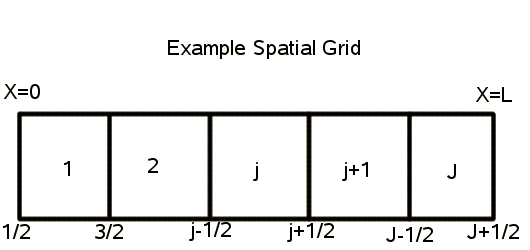
\includegraphics[width=\imgwidth,height=\imgheight]{SimpleGrid}}
		\end{picture}
		\caption{\label{fig:SimpleGrid} Simple one-dimensional orthogonal grid.}
		%\end{minipage} %\hfill
	\end{center}
\end{figure}

	The divergence of the flux in equation \ref{finalDiffusion} can be expressed as a simple edge centered differencing;
	\begin{equation}
	\label{dStream}
	\bar{\nabla}\cdot{F(\nu)}={F_{j+{1\over{2}}}(\nu)-F_{j-{1\over{2}}}(\nu)\over{\Delta{x_j}}}.
	\end{equation}
	The flux on either side of the cell edge can be written using Fick's law (equation \ref{FicksLaw});
	\begin{equation}
	\label{dStream2}
	F_{j+{1\over{2}}}^-(\nu)=-D_{j}(\nu){\left(E_{j+{1\over{2}}}(\nu)-E_j(\nu)\right)\over{{\Delta{x_{j}}\over{2}}}}
	\end{equation}
	and
	\begin{equation}
	\label{dStream3}
	F_{j+{1\over{2}}}^+(\nu)=-D_{j+1}(\nu){\left(E_{j+1}(\nu)-E_{j+{1\over{2}}}(\nu)\right)\over{{\Delta{x_{j+1}}\over{2}}}}.
	\end{equation}
	Finally, given the assumption that the flux is continuous it can be seen that
	\begin{equation}
	\label{dStream5}
	F_{j+{1\over{2}}}^+(\nu)=F_{j+{1\over{2}}}^-(\nu).
	\end{equation}
	The flux at the cell edge can now be written in terms of the cell centered energy density by combining equations \ref{dStream2} through \ref{dStream5}: 
	\begin{equation}
	\label{dStream6}
	F_{j+{1\over{2}}}(\nu)=-{2D_j(\nu)D_{j+1}(\nu)\over{\Delta{x_{j+1}}D_j(\nu)+\Delta{x_{j}}D_{j+1}(\nu)}}\left(E_{j+1}(\nu)-E_{j}(\nu)\right).
	\end{equation}
% 	Similarly, it can be shown that
% 	\begin{equation}
% 	\label{dStream7}
% 	F_{j-{1\over{2}}}(\nu)=-{2D_{j-1}(\nu)D_{j}(\nu)\over{\Delta{x_{j}}D_{j-1}(\nu)+\Delta{x_{j-1}}D_{j}(\nu)}}\left(E_{j}(\nu)-E_{j-1}(\nu)\right).
% 	\end{equation}
	With this new expressions for the photon flux at the cell edge the divergence of the flux becomes:
	\begin{eqnarray}
	\label{dStream8}
	&&\bar{\nabla}\cdot{F(\nu)}=-c{2D_j(\nu)D_{j+1}(\nu)\over{\Delta{x_j}\left(\Delta{x_{j+1}}D_j(\nu)+\Delta{x_{j}}D_{j+1}(\nu)\right)}}\left(E_{j+1}(\nu)-E_{j}(\nu)\right)\nonumber \\ & & +c{2D_{j-1}(\nu)D_{j}(\nu)\over{\Delta{x_j}\left(\Delta{x_{j}}D_{j-1}(\nu)+\Delta{x_{j-1}}D_{j}(\nu)\right)}}\left(E_{j}(\nu)-E_{j-1}(\nu)\right).
	\end{eqnarray}
	
	Inserting equation \ref{dStream8} into equation \ref{finalDiffusion} yields a tridiagonal system of equations for the cell centered energy density:
	\begin{equation}
	\label{disDiff}
	B_j(\nu)E_{j-1}^{t+1}(\nu) + D_j(\nu)E_j^{t+1}(\nu) + C_j(\nu)E_{j+1}^{t+1}(\nu) = Q^t_j(\nu),
	\end{equation}
	where
	\begin{equation}
	\label{distDiffB}
	B_j(\nu)=-{c2\Delta{t}D_{j-1}D_{j}\over{\Delta{x_j}\left(\Delta{x_{j}}D_{j-1}+\Delta{x_{j-1}}D_{j}\right)}},
	\end{equation}
	\begin{equation}
	\label{distDiffC}
	C_j(\nu)=-{c2\Delta{t}D_{j}(\nu)D_{j+1}(\nu)\over{\Delta{x_j}\left(\Delta{x_{j+1}}D_{j}(\nu)+\Delta{x_{j}}D_{j+1}(\nu)\right)}},
	\end{equation}
	\begin{equation}
	\label{distDiffD}
	D_j(\nu)=1+c\Delta{t}\sigma(\nu){f(T_j)}+c\Delta{t}\sigma(\nu){(1-f(T_j))} -A(\nu) -C(\nu), 
	\end{equation}
	and
	\begin{equation}
	\label{Q_j}
	Q_j(\nu)=c\Delta{t}\sigma_p(T_j)f(T_j)aT^4_j+c\Delta{t}{\sigma(\nu)b(\nu,T_j)\over{\sigma_p}}{\int{d\nu}E^{t+1}_j(\nu)\sigma_s(\nu)}+E_j(\nu).
	\end{equation}

\belowSubSecSkip

%==================%
% SubSubSection:   %
%    Energy Discretization %
%==================%
\subsubsection{Boundary Cells}
\label{sec:Transport-Discret-Boundary-Cells}

\noindent
	\indent There are two boundary conditions considered in this paper; an albedo boundary condition and an incident boundary flux. The albedo boundary condition can be described as a boundary that reflects some fraction($\gamma$) of the exiting boundary partial flux back into the boundary cell. The partial flux entering the right surface boundary can be expressed as 
	\begin{equation}
	\label{enteringPartialFlux}
	f_{{1\over{2}}}^-(\nu)={1\over{4}}E_{{1\over{2}}}(\nu)-{1\over{2}}F_{{1\over{2}}}(\nu),
	\end{equation}
	and the partial flux exiting the surface through the unit normal can be expressed as
	\begin{equation}
	\label{exitingPartialFlux}
	f_{{1\over{2}}}^+(\nu)={1\over{4}}E_{{1\over{2}}}(\nu)+{1\over{2}}F_{{1\over{2}}}(\nu).
	\end{equation}
	The total flux can be expressed as the difference of the partial flux incident on and exiting the left surface boundary.
	\begin{equation}
	\label{totalFlux}
	F_{{1\over{2}}}(\nu)={f_{{1\over{2}}}}^{-}(\nu)-{f_{{1\over{2}}}^+(\nu)}
	\end{equation}
	
	Given the case of an albedo boundary, the equation for the total flux (equation \ref{totalFlux}) becomes
	\begin{equation}
	\label{albedoTotalFlux}
	F_{{1\over{2}}}(\nu)=\gamma{f_{{1\over{2}}}}^{+}(\nu)-{f_{{1\over{2}}}^+(\nu)},
	\end{equation}
	where $\gamma$ denotes the precentage of the exiting flux that is reflected back into the system. Combining Fick's law, the partial fluxes, and the total flux (equation \ref{FicksLaw}, \ref{enteringPartialFlux}, \ref{exitingPartialFlux}, and \ref{albedoTotalFlux}) and solving for the left boundary flux in terms of $\gamma$ and $E_{j}(\nu)$ yields;
	\begin{equation}
	\label{albedoBoundar}
	F_{{1\over{2}}}(\nu)=-{2D_1(\nu)E_1(\nu)\left({1-\gamma\over{1+\gamma}}\right)\over{\Delta{x_1}\left(\left({1-\gamma\over{1+\gamma}}\right)+{4D_1(\nu)\over{\Delta{x}_1}}\right)}}.
	\end{equation}
	Similarly the flux for a right albedo boundary condition can be expressed as
	\begin{equation}
	\label{albedoBoundar}
	F_{J+{1\over{2}}}(\nu)={2D_J(\nu)E_J(\nu)\left({1-\gamma\over{1+\gamma}}\right)\over{\Delta{x_J}\left(\left({1-\gamma\over{1+\gamma}}\right)+{4D_J(\nu)\over{\Delta{x}}}\right)}}.
	\end{equation}

	For the case where the system has an incident flux on the left boundary, flux can be expressed as
	\begin{equation}
	\label{incidentPartialFlux}
	f_{{1\over{2}}}^-(\nu)={1\over{4}}E_{{1\over{2}}}(\nu)-{1\over{2}}F_{{1\over{2}}}(\nu)+F_o(\nu).
	\end{equation}
	Using this equation for the partial incident flux and the other equations used to solve the albedo boundary condition above results in the following expression for the total left boundary flux;
	\begin{equation}
	\label{incidentBoundaryCondition}
	F_{{1\over{2}}}(\nu)={2D_1(\nu)E_1(\nu)\left({4F_o(\nu)\over{c}}-E_1(\nu)\right)\over{\Delta{x_1}\left(1+{4D_1(\nu)\over{\Delta{x}_1}}\right)}}.
	\end{equation}
	Similarly the flux for a right incident flux boundary condition can be expressed as
	\begin{equation}
	\label{incidentBoundaryCondition}
	F_{J+{1\over{2}}}(\nu)=-{2D_J(\nu)E_J(\nu)\left({4F_o(\nu)\over{c}}-E_J(\nu)\right)\over{\Delta{x_J}\left(1+{4D_J(\nu)\over{\Delta{x}_J}}\right)}},
	\end{equation}
	where $F_o(\nu)$ denotes the incident partial flux.

\belowSubSecSkip

%=====================================================================%
% SubSection:                        	                              %
%     Transport: Summary %
%=====================================================================%
\subsection{Summary}
\label{sec:Transport-Summary}

\noindent
	\indent In this section the radiative transfer equation and material energy balance equation were transformed into an ``effective scattering'' diffusion equation. This diffusion equation was then discretized in space to generate a tridiagonal system for the cell-centered energy density at the next time step. Discretized forms of the boundary conditions were also derived



%=================================================%
% Section:                        	              %
%    Implicit Monte Carlo%
%=================================================%

\begin{center}
\section{Implicit Monte Carlo}
\label{sec:MonteCarlo}
\end{center}

%====================================================================%
% SubSection:                        	                             %
%    Implicit Monte Carlo: Introduction %
%====================================================================%
\aboveSubSecSkip

\subsection{Introduction}
\label{sec:MonteCarlo-Intro}

\noindent
	\indent Monte Carlo methods have been used extensively in the field of nuclear physics. This chapter will describe in detail how a linear system  with certain characteristics can be solved via a Monte Carlo algorithm[Ham. 1964]. This linear system must be diagonally dominant and the off diagonal terms must be negative. Though it might be possible to solve linear systems that do not have these properties with this method, it is not included in the scope of this work and should be further explored for the needs of running problems on non-orthogonal meshes.
			
\belowSubSecSkip

%====================================================================%
% SubSection:                        	                             %
%    Implicit Monte Carlo: Monte Carlo%
%====================================================================%
\aboveSubSecSkip

\subsection{Monte Carlo Basics}
\label{sec:MonteCarlo-MC}

\noindent
	\indent A Monte Carlo method consits of the generation of a finite number of particle histories that are controlled by known probabilities of the system of interest. For demonstrative purposes, we will use an example of a fixed source problem with scattering. In this system, there are two possible interactions; scatter or absorption. First it is necessary to define a probability distribution function (PDF). This function describes the probability that a variable (x) will lie in the range of two values (a and b). A probability distribution function can be written as a function of the probability density function $f(x)$[Lew. 1993];
	\begin{equation}
	 P(x)=\int_a^b\delta x' f(x')
	\end{equation}
	A probability density function is a function which describes the probability at value x. In the example problem, the probability that a particle will have an interaction over a distance (x) $[cm]$ can be written as
	\begin{equation}
	 f(x)=e^{-x{\sigma_t}},
	\end{equation}
	where $\sigma_t$ is the total opacity $[1/cm]$. The total opacity is equal to the sum of the scattering opacity and the absorption opacity. Now it is necessary to define the cumulative probability distribution function (CPDF). This function represents the probability that some random variable x' is less then or equal to x. This can be written as;
	\begin{equation}
	 F(x)=\int_0^xf(x')dx'.
	\end{equation}
 	Given the definition of the example probability density function, the CPDF can be expressed as;
	\begin{equation}
	 F(x)=1-e^{{-x{\sigma_t}}}.
	\end{equation}
	Knowing that the value of a CPDF will always range between zero and one, it is possible to select a random number, between zero and one, to determine the distance (x) traveled by the particle before a collision[Lew. 1993]. This is done by setting $F(x)$ equal to a random number $(\zeta)$ and then solving for x. Knowing the location of the next collision it is now necessary to determine the collision type.

	It is possible to determine the collision type by constructing another probability density function. For the example problem there are two types of possible interactions; scattering and absorption. The probability density function of the collision types will consits of a histogram with two values.
	\[
	 f(k)=\left(
	 \begin{array}{c c}
	   {\sigma_s\over{\sigma_t}}\hspace{0.25in} & \, k_0\leq k\leq k_1 \\
	   {\sigma_a\over{\sigma_t}}\hspace{0.25in} & \, k_1<k\leq k_2  \\
	 \end{array}
	 \right)
	\]
	Where the range between $k$ denotes a collision type. The CPDF is constructed by integrating this histogram from $k_0$ to some value k. If this integration is performed and $F(k)$ is set equal to a random number $(\zeta)$ between zero and one, the collision type can be selected using;
	\[
	 k(\zeta)=\left(
	 \begin{array}{c  c}
	    scatter\hspace{0.25in} \, 0\leq\zeta\leq{\sigma_s\over{\sigma_t}}\\
	    absorbed\hspace{0.25in} \, {\sigma_s\over{\sigma_t}}<\zeta\leq1\\
	 \end{array}
	 \right).
	\]
	If the collision type is an absorption, the weight of the particle is ``tallied''; its weight is added to a sum of absorption events for its current location. If the particle is scattered, a new direction and frequency is chosen and the particle continues to the next interaction location.

	The IMD code presented in this work uses the probabilities defined in the next section to create PDFs and CPDFs which are then used to create and transport particles. This work also uses absorption suppression combined with Russian Roulette as a variance reduction technique. Absorption suppression works by tallying the probability of an absorption event multiplied by the current particle weight at the beginning of every random walk, rather than including it in the CPDF. This is done until a particle dies (is tallied into census or leaves the problem) or falls below a designated weight and Russian Roulette occurs[Lew. 1993]. During Russian Roulette, the particle is either killed or its weight is increased according to a user designated probability. Russian Rouletting is a unbiased way of ending a particle history[Lew. 1993]. Absorption suppression with Russian Roulette accurately accounts for the absorption probability and it reduces the variance in the system.
			
\belowSubSecSkip


%=====================================================================%
% SubSection:                        	                              %
%     Implicit Monte Carlo: Linear System%
%=====================================================================%
\subsection{Linear System}
\label{sec:MonteCarlo-Linear-System}

\noindent
	\indent There are a few very important properties that a matrix must have in order for a probabilistic interpretation of the linear system to be stable. The matrix must be positively diagonally dominant and the fringe terms must be negative. This forces the probabilities to be positive and finite. The linear system that is being solved in this paper is a simple tridiagonal system that is diagonally dominant and has the correct sign for the matrix terms (equation \ref{disDiff}). The system can be written as
	\begin{equation}
	\label{linearSystem}
	Ax=b,
	\end{equation}
	where $A$ is the coefficient matrix which for a tridiagonal system can be expressed as follows;
	\[
	\left(
	\begin{array}{ c c c c c c c c c c c c c}
	D_1 & \, & C_2 & \, & 0  & \, & . & \, & . & \, & . & \, & 0 \\
	B_1 & \, & D_2 & \, & C_3  & \, & . & \, & \, & \, & \, & \, & . \\
	0 & \, & B_2 & \, & D_3  & \, & C_4 & \, & . & \, & \, & \, & . \\
	. & \, & . & \, & .  & \, & . & \, & . & \, & . & \, & . \\
	. & \, & \, & \, & .  & \, & B_{N-3} & \, & D_{N-2} & \, & C_{N-1} & \, & 0 \\
	. & \, & \, & \, & \,  & \, & . & \, & B_{N-2} & \, & D_{N-1} & \, & C_{N} \\
	0 & \, & . & \, & .  & \, & . & \, & 0 & \, & B_{N-1} & \, & D_{N} \\
	\end{array}
	\right)
	\left(
	\begin{array}{ c }
	E_0 \\
	. \\
	. \\
	. \\
	. \\
	. \\
	E_N 
	\end{array}
	\right)
	=
	\left(
	\begin{array}{ c }
	Q_0 \\
	. \\
	. \\
	. \\
	. \\
	. \\
	Q_N 
	\end{array}
	\right),
	\]
	where B, C, and D are defined by equations \ref{distDiffB}, \ref{distDiffC}, and \ref{distDiffD} respectively, $E_j$ denotes the photon energy density at the current time step in cell $j$, and $Q_j$ is the source term expressed in equation \ref{Q_j}.
	
	To put this expression in a form that can be used to solve the linear equations via Monte Carlo, we split $A$ into its diagonal and off-diagonal components;
	\begin{equation}
	\label{fring}
	F=A-D,
	\end{equation}
	where $D$ is defined by
	\[
	D=
	\left(
	\begin{array}{ c c c c c c c c c }
	D_1 & \, & 0 & \, & . & \, & . & \, & 0 \\
	0 & \, & D_2 & \, & . & \, & \, & \, & . \\
	. & \, & . & \, & . & \, & . & \, & . \\
	. & \, & \, & \, & .  & \, & D_{N-1} & \, & 0  \\
	0 & \, & . & \, & . & \, & 0 & \, & D_{N} \\
	\end{array}
	\right).
	\]
	Using the definition in equation \ref{fring}, it is possible to rewrite the linear system as
	\begin{equation}
	Fx+Dx=b.
	\end{equation}
	This can be rearranged to get the form necessary to solve the linear equations with a Monte Carlo algorithm[Ham. 1964].
	\begin{equation}
	\label{linearMC}
	x=Hx+D^{-1}b
	\end{equation}
	where $H$ can be expressed as;
	\begin{equation}
	H=-D^{-1}F
	\end{equation}
	or
	\[
	H=
	\left(
	\begin{array}{ c c c c c c c}
	0  & -{C_2\over{D_2}}  & 0   & .  & .  & .  & 0 \\
	-{B_1\over{D_1}}  & 0  & -{C_3\over{D_3}}  & .  & \, & \,  & . \\
	0 &  -{B_2\over{D_2}} & 0  & -{C_4\over{D_4}} & . & \, & . \\
	. & . & . & . & . & . & . \\
	. & \, & . & -{B_{N-3}\over{D_{N-3}}} & 0 & -{C_{N-1}\over{D_{N-1}}} & 0 \\
	. & \, & \, & . & -{B_{N-2}\over{D_{N-2}}} & 0 & -{C_{N}\over{D_{N-1}}} \\
	0 & .  & . & . & 0 & -{B_{N-1}\over{D_{N-1}}} & 0 \\
	\end{array}
	\right).
	\]

	For simplicity of the probability derivations, matrix $A$ can be broken up into the streaming operator terms plus the remaining terms in the coefficient matrix. We will denote these two matrices as $\mathcal{F}$ and $\mathcal{D}$. Where these terms denote the streaming operator (equation \ref{dStream8}) and the remaining terms in the coefficient matrix respectively. 
	\begin{equation}
	 \mathcal{D}=A-\mathcal{F}
	\end{equation}
	

\belowSubSecSkip

%=====================================================================%
% SubSection:                        	                              %
%      Implicit Monte Carlo: Probabilities %
%=====================================================================%
\subsection{Probabilities}
\label{sec:MonteCarlo-Probabilities}	

\noindent
	\indent It can be seen that the diffusion equation (equation \ref{finalDiffusion})  in  a single cell with a single frequency or frequency group ($\nu$) can be expressed as;
	\begin{eqnarray}
	\label{ProbabilitiesDiffusion}
	& &{1\over{c}}{\Delta{E(\nu)_j}\over{\Delta{t}}} + \sum_{i=1}^N\mathcal{F}_{ij}^{t+1}(v)E^{t+1}_i(\nu)=\nonumber \\& & -E^{t+1}_j(\nu)(\sigma_{s_j}(\nu)+\sigma_{a_j}(\nu))+{b(\nu,T_j)\sigma(\nu)\over{\sigma_p(T_j)}}(\nu)\sigma_p(T_j)f(T_j)aT_j^{t^4}\nonumber \\& & +{\sum_{\nu_{k-1}}^{\nu_k}\sigma(\nu)\int_{\nu_{k-1}}^{\nu_k}d\nu b(\nu,T_j)\over{\sigma_p(T_j)}}{\int{d\nu}E^{t+1}_j(\nu)\sigma_{s_j}(\nu)}.
	\end{eqnarray}
	In matrix form it can also be seen from equation \ref{linearMC} that the photon energy density in a single cell for a single frequency can be expressed as;
	\begin{equation}
	\label{componentMC}
	E^{t+1}_j(\nu)=D_j^{-1}(\nu)Q_j(\nu)+\sum_{i=1}^N{h_{ji}(\nu)E_i(\nu)}.
	\end{equation}
	These equations will be important later in this section.

	$P_{th}(\nu)$ is the probability that a photon will have the frequency $\nu$ when it is emitted from the material body. This probability can be expressed as;
	\begin{equation}
	\label{thermalDistribution}
	P_{th_j}(\nu)={b(\nu,T_j)\sigma(\nu)\over{\int^\infty_0d\nu{b(\nu,T_j)\sigma(\nu)}}}={b(\nu,T_j)\sigma(\nu)\over{\sigma_p(T_j)}}.
	\end{equation}
	For a multigroup method this probability would be expressed for group k as;
	\begin{equation}
	\label{multigroupThermalDistribution}
	P_{th,k_j}={\sum_{\nu_{k-1}}^{\nu_k}\sigma(\nu)\int_{\nu_{k-1}}^{\nu_k}d\nu b(\nu,T_j)\over{\sigma_p(T_j)}}.
	\end{equation}
	The Taylor expansion of the Planckian, as described by Barnett and Canfield [Bar. 1970], is integrated analytically and then used to calculate the Planckian. The integrated Taylor expansion can be carried out to as high an order as the user desires. Each extension of the Taylor expansion increases the accuracy of the integral calculation.
 
	The problems we consider do not have real scattering this is an effective scattering system which means it is known that a scattering event is an approximation for a quick absorption and reemission. This means that the probability of a photon with frequency $\nu$ being emitted after a scatter is equal to the probability of a thermal photon being emitted at the frequency $\nu$. 
	\begin{equation}
	P_{th}(\nu)=P_s(\nu).
	\end{equation}
	
	The newly created particles must adhere to some interaction probabilities. The most important of these probabilities is the {\it census probability}. Census, in this case, means that a particle will remain in the cell at the next time step. This probability can be expressed as
	\begin{equation}
	\label{censusProb}
	P^c_j(\nu)={1\over{D_j(\nu)}},
	\end{equation}
	where $D$ represents the diagonal terms expressed for internal cells in equation \ref{distDiffD}. As $\Delta{t}$ approaches zero, the probability of census goes to one, and as the opacity gets very large the probability of census will decrease toward zero. The {\it scattering probability} can be defined as 
	\begin{equation}
	\label{absorptionProb}
	P^s_j(\nu)={c\Delta{t}\sigma(\nu){(1-f(T_j))}\over{D_j(\nu)}}.
	\end{equation}
	The scattering probability will go to zero as $f$ approaches one. The {\it leakage probability}, 
	\begin{equation}
	\label{leakageProb}
	P^l_{ij}(\nu)=h_{ij}(\nu)={\mathcal{F}_{ji}(\nu)\over{D_j(\nu)}},
	\end{equation}
	is the probability that a particle will leak from a neighboring cell $i$ into the current cell $j$. This term will be always positive if the terms of matrix $H$ are positive. This means that the fringe terms of matrix $A$ must be negative. The {\it total leakage probability},  
	\begin{equation}
	\label{totalLeakageProb}
	P^{Tl}_j(\nu)=\sum_{i=1}^N{h_{ji}(\nu)}=\sum_{i=1;i\neq{j}}^N{\mathcal{F}_{ji}(\nu)\over{D_j(\nu)}},
	\end{equation}
	is the probability of a particle leaking out of cell $j$. The total probability of leakage will always be less than or equal to one because the denominator can be expressed as a sum which contains all terms in the numerator.  The total leakage probability is equal to zero if the cell is infinitely large. The {\it source probability} can be written as
	\begin{equation}
	\label{sourceProb}
	P^q_j(\nu)={Q_j(\nu)\over{\sum\limits_{i=1}^N{Q_i(\nu)}}},
	\end{equation}
	where $Q_i$ and $Q_j$ are terms in the source vector $Q$. Again, because the sum in the denominator always contains the term in the numerator, the probability expressed in equation \ref{sourceProb} will range between zero and one.

	The total radiation energy in the system can be expressed as;
	\begin{equation}
	\label{totalEnergy}
	E_T=\sum\limits_{i=1}^N\left(c\Delta{t}\sigma_pfaT_i^4V_i+\int^\infty_0d\nu E_i^t(\nu)V_i\right).
	\end{equation}
	If the total number of particles to be created is equal to $N$, then the number of particles created in a single frequency in a cell $j$ can be expressed as
	\begin{equation}
	\label{censusTally}
	N^c_j(\nu)=N\left({c\Delta{t}b(\nu,T_j)\sigma_a(\nu) aT_j^4V_j+E_j^t(\nu)V_j\over{E_T}}\right).
	\end{equation}
	This also means that the weight of each particle created can be expressed as;
	\begin{equation}
	\label{particleWeight}
	w_j(\nu)={(c\Delta{t}b(\nu,T)\sigma_a(\nu) aT_j^4V_j+E_j^t(\nu)V_j)\over{N^c_j(\nu)}}.
	\end{equation}
	The photon energy density at any one time in a given cell $j$ can be expressed as
	\begin{equation}
	\label{censusTally}
	E_j(\nu)\equiv\lim_{N_j \to +\infty}P^c_j(\nu)w_j(\nu)N_j(\nu).
	\end{equation}
	where $ P^c_j(\nu) $ is the census probability for cell $j$, $w_j(\nu)$ is the weight of each particle, and $N_j(\nu)$ is the number of particles with frequency $\nu$ in the cell $j$. This should be equal to the total number of particles with frequency $\nu$ that are created in the cell, enter the cell from surrounding cells, and scatter in the cell from a different frequency into frequency $\nu$.
	\begin{equation}
	\label{numParticles} 
	N_j(\nu)=\sum_{i=1}^N{P^l_{ij}(\nu)}N_i(\nu)+N^c_j(\nu)+P_s(\nu)\int^\infty_0d\nu' P^s(\nu')N_j(\nu')
	\end{equation}
	Now it is possible to substitute equation \ref{numParticles} into equation \ref{censusTally}.
	\begin{eqnarray}
	\label{censusTally2}
	E_j(\nu)=& &P^c_j(\nu)w_j(\nu)\sum_{i=1;i\neq{j}}^N{P^l_{ij}(\nu)}N_i(\nu)+\\& & \nonumber
		P^c_j(\nu)w_j(\nu)N^c_j(\nu)+P^c_jw_j(\nu)P_s(\nu)\int^\infty_0d\nu' P^s(\nu')N_j(\nu')
	\end{eqnarray}
	The source term in equation \ref{censusTally2} can be rewritten such that
	\begin{equation}
	\label{censusSourceTerm}
	P^c_j(\nu)w_j(\nu)N^c_j(\nu)={P_{th}(\nu)c\Delta{t}\sigma_pfaT_t^4+E_j^t(\nu)\over{D_j(\nu)}}.
	\end{equation}
	Using equations \ref{leakageProb}, \ref{censusTally}, and \ref{censusProb} the leakage term can be rewritten such that
	\begin{eqnarray}
	\label{censusLeakageTerm}
	P^c_j(\nu)w_j(\nu)\sum_{i=1}^N{P^l_{ij}(\nu)}N_i(\nu)& &={1\over{D_j}}{\sum_{i=1;i\neq{j}}^N{\mathcal{F}_{ji}(\nu)w_pN_i\over{D_i(\nu)}}} \\& & \nonumber
	={\sum_{i=1;i\neq{j}}^N{\mathcal{F}_{ji}(\nu)E_i\over{D_j(\nu)}}}.
	\end{eqnarray}
	The scatter term of equation \ref{censusTally2} can now be rewritten using equations \ref{censusTally} and \ref{censusProb} yielding;
	\begin{equation}
	\label{censusScatteringTerm}
	P^c_j(\nu)w_j(\nu)P_s(\nu)\int^\infty_0d\nu' P^s(\nu')N_j(\nu')={P_s(\nu)\over{D_j(\nu)}}{\int{d\nu'}E_j(r,\nu')\sigma(\nu')_s}.
	\end{equation}
	Rewriting equation \ref{censusTally2} with equations \ref{censusSourceTerm}, \ref{censusLeakageTerm}, and \ref{censusScatteringTerm} and replacing the probabilities with associated matrix terms yields;
	\begin{equation}
	\label{censusTallyFinal}
	E_j=Q_jD_j^{-1}+\sum_{i=1}^N{h_{ji}E_i}.
	\end{equation}
	Using equation \ref{censusTally2} with equations \ref{censusSourceTerm}, \ref{censusLeakageTerm}, and \ref{censusScatteringTerm} and multiplying $D_j\over{c\Delta{t}}$ by both sides will yield the following result;
	\begin{eqnarray}
	\label{ProbabilitiesDiffusion}
	& &{1\over{c}}{\Delta{E(\nu)_j}\over{\Delta{t}}} + \sum_{i=1}^N\mathcal{F}_{ij}(v)E_i(\nu)=\nonumber \\& & -E_j(\nu)(\sigma_s(\nu)_j+\sigma_a(\nu)_j)+P_{th}(\nu)\sigma_pfaT^4\nonumber \\& & +P_s({\nu}){\int{d\nu}E_j(\nu)\sigma(\nu)_s}.
	\end{eqnarray}
	This shows that if the system of probabilities defined above was solved with an infinite number of particles $E_j(\nu)$ would be equal to $E^{t+1}_j(\nu)$.

	For the right albedo boundary condition, the diagonal term can be expressed as
	\begin{eqnarray}
	\label{albedoBoundaryD}
	&&D_a=1+c\Delta{t}\sigma(\nu){f(T_J)}+c\Delta{t}\sigma(\nu){(1-f(T_J))}\nonumber \\ && +{c2\Delta{t}D_{J}(\nu)D_{J-1}(\nu)\over{\Delta{x_J}\left(\Delta{x_{J-1}}D_{J}(\nu)+\Delta{x_{J}}D_{J-1}(\nu)\right)}}+{c2\Delta{t}D_J(\nu)\left({1-\gamma\over{1+\gamma}}\right)\over{\Delta{x_J}\left(\left({1-\gamma\over{1+\gamma}}\right)+{4D_J(\nu)\over{\Delta{x}_J}}\right)}}.
	\end{eqnarray}
	For the incident flux boundary condition, the diagonal term and the source term can be expressed as 
	\begin{eqnarray}
	\label{incidentBoundaryD}
	&&D_{if}=1+c\Delta{t}\sigma(\nu){f(T_J)}+c\Delta{t}\sigma(\nu){(1-f(T_J))}\nonumber \\ && +{c2\Delta{t}D_{J}(\nu)D_{J-1}(\nu)\over{\Delta{x_J}\left(\Delta{x_{J-1}}D_{J}(\nu)+\Delta{x_{J}}D_{J-1}(\nu)\right)}}+{c2\Delta{t}D_J(\nu)\over{\Delta{x_J}\left(1+{4D_J(\nu)\over{\Delta{x}_J}}\right)}}\end{eqnarray}
	and
	\begin{equation}
	\label{boundarySourceQ}
	Q_{if}=c\Delta{t}\sigma_p(T_J)f(T_J)aT^{t^4}_J+E_J^t+{c8\Delta{t}D_J(\nu){F_o}\over{\Delta{x_J}\left(1+{4D_J(\nu)\over{\Delta{x}_J}}\right)}}.
	\end{equation}
	For the boundary cells it is necessary to define a boundary leakage probability ($P^{b}$) and a boundary source probability $P^{b,q}$. The albedo boundary leakage probability is expressed as;
	\begin{equation}
	\label{boundaryLeakageProbAl}
	P^{bl}_a(\nu)={{c2\Delta{t}D_J(\nu)\left({1-\gamma\over{1+\gamma}}\right)\over{\Delta{x_J}\left(\left({1-\gamma\over{1+\gamma}}\right)+{4D_J(\nu)\over{\Delta{x}}}\right)}}\over{D_a(\nu)}}.
	\end{equation}
	The incident flux boundary leakage probability is expressed as;
	\begin{equation}
	\label{boundaryLeakageProbIF}
	P^{bl}_{if}(\nu)={{c2\Delta{t}D_J\over{\Delta{x_J}\left(1+{4D_J(\nu)\over{\Delta{x}}}\right)}}\over{D_{if}(\nu)}}.
	\end{equation}
	For these boundary cells the source probability shown in equation \ref{sourceProb} would remain true with the new value of $Q$ defined in equation \ref{boundarySourceQ} for the incident flux boundary, or the value of $Q$ defined by equation \ref{Q_j} for the albedo boundary. If the appropriate boundary leakage probability, either albedo or incident flux depending on user specifications, was add to the total leakage probability defined by equation \ref{totalLeakageProb} the census tally (equation \ref{censusTally2}) will yields the correct results for the right boundary cell equations. This will also be true for the left boundary conditions as defined in Section \ref{sec:Transport-Discret-Boundary-Cells}.
	
	If an infinite number of particles were simulated, this method would yield the result as defined in equation \ref{linearMC}. Using this method, it is possible to solve for the photon energy density at the end of a single time step. However, it is not possible to recalculate the material energy density, which is necessary to calculate time steps in sequence, without including more probabilities and tallies. To solve for the material energy density at the end of the time step it is necessary to solve the equation of state (equation \ref{EqState}). This is done by creating an emission source tally and an absorption tally. The absorption tally can be defined as the amount of energy absorbed into the material over a time step
	\begin{equation}
	\label{absorptionTally}
	E^a_j(\nu)=P^a_j(\nu)w_pN_j
	\end{equation}
	where $P^a_j(\nu)$ is the probability of absorption into the material of cell j. The {\it absorption probability} can be expressed as;
	\begin{equation}
	\label{absorptionProb}
	P^a_j(\nu)={c\Delta{t}\sigma(\nu){f(T_j)}\over{D_j(\nu)}}.
	\end{equation}
	As the Fleck factor ($f(T_j)$) approaches zero, the probability of absorption goes to zero. This is true for systems that are purely scattering. As the opacity gets very large, the probability of absorption goes to one. If equation \ref{absorptionProb} is subsituted into equation \ref{absorptionTally} the following expresssion can be made for the energy absorbed in cell j;
	\begin{equation}
	\label{energyAbsorbed}
	E^a_j(\nu)={c\Delta{t}\sigma(\nu){f(T_j)}w_pN_j\over{D_j(\nu)}}=c\Delta{t}\sigma(\nu){f(T_j)}P^c_j(\nu)w_pN_j.
	\end{equation}
	Given the definition in equation \ref{censusTally2}
	\begin{equation}
	\label{reducedEnergyAbsorbed}
	E^a_j(\nu)=\int{d\nu}c\Delta{t}\sigma(\nu){f(T_j)}E_j(\nu).
	\end{equation}
	Knowing that $E_j(\nu)$ is an approximation for $E^{t+1}_j(\nu)$ equation \ref{EqState} can be rewritten using equation \ref{reducedEnergyAbsorbed}.
	\begin{equation}
	\label{EqState}
	\Delta{E_{m_j}}=\int{d\nu}c\Delta{t}\sigma(\nu){f(T_j)}E_j(\nu)-c\Delta{t}\sigma_p(T_j) f(T_j){aT^{t^4}_j}
	\end{equation}
	This shows that the change in the material energy density can be determined using the absorption tally defined above.

\belowSubSecSkip


%=====================================================================%
% SubSection:                        	                              %
%     Implicit Monte Carlo: Summary %
%=====================================================================%
\subsection{Summary}
\label{sec:MonteCarlo-Summary}

\noindent
	\indent This section describes the matrix manipulations required to get the linear system in a form that is solvable via Monte Carlo. After the matrix manipulations are performed the probabilities are derived along with their associated proofs to be used with the Monte Carlo Method. This includes the development of the tallies which are required to produce the photon energy density and the material energy density at the next time step. This section also includes the frequency distribution functions associated with the thermal and scattering sources.



%=================================================%
% Section:                        	              %
%    Difference Formulation%
%=================================================%

\begin{center}
\section{Difference Formulation}
\label{sec:DifferenceFormulation}
\end{center}

%====================================================================%
% SubSection:                        	                             %
%    Difference Formulation: Introduction %
%====================================================================%
\aboveSubSecSkip

\subsection{Introduction}
\label{sec:DifferenceFormulation-Intro}

\noindent
	\indent In this chapter the difference formulation will be derived for the frequency dependent implicit diffusion and material energy balance equations. We demonstrate that the application of the difference formulation does not change the converged solution. The difference formulation is a variance reduction technique which changes the source of the problem to focus the computational work on parts of the system that are rapidly changing[Bro 2005]. The difference formulation in-dues subtracting a differential time and streaming operator applied to the Planckian source from both sides of the equation. This results in a new ``differenced'' energy density, defined as;
	\begin{equation}
	\label{newEnergyDensity}
	E^{t+1}_{d}(r)=E^{t+1}(r)-B{(v,T_{d}(r))}.
	\end{equation}
	Here $B$ denotes the Planck distribution (equation \ref{newPlanck}) integrated over all angle and $T_d(r)$ is the ``differencing'' temperature used for the subtracted Planckian source.

\belowSubSecSkip

%=====================================================================%
% SubSection:                        	                              %
%     Difference Formulation: Diffusion Equation                      %
%=====================================================================%
\subsection{Diffusion Equation}
\label{sec:DifferenceFormulation-Diffusion-Equation}

\noindent
	\indent The photon energy density differencing shown in equation \ref{newEnergyDensity} can be used to rewrite the diffusion equation (equation \ref{finalDiffusion}) in a new form;
	\begin{eqnarray}
	\label{differenceFormulation1}
	& &{1\over{c}}{\Delta{E_d(r,\nu)}\over{\Delta{t}}} + \nabla{F^{t+1}_{d}(r,\nu)}=\nonumber \\& & -E^{t+1}_{d}(r,\nu)\sigma(\nu)+{b(\nu,T(r))}\sigma(\nu)f(T(r)) aT^4(r)\nonumber \\& & +{\sigma(\nu)b(\nu,T(r))\over{\sigma_p}}{\int{d\nu}E^{t+1}_{d}(r,\nu)\sigma(\nu)(1-f(T(r)))}\nonumber \\& &
	-b(\nu,T_d(r))aT_d^4(r)\sigma(\nu)\nonumber \\& &
	+{\sigma(\nu)b(\nu,T(r))\over{\sigma_p}}{\int{d\nu}b(\nu,T_d(r))aT_d^4(r)\sigma(\nu)(1-f(T(r)))}\nonumber \\& &
	-{1\over{c}}{\Delta{b(\nu,T_d(r))aT_d^4(r)}\over{\Delta{t}}} - \nabla{\left(-D\nabla{b(\nu,T_d(r))}aT_d^4(r)\right)},
	\end{eqnarray}
	where the $T_d$ is a user definable temperature chosen for the differencing. If the new scattering term containing the normalized Planckian for the ``differencing'' temperature in equation \ref{differenceFormulation1} is integrated and expanded, the new form of the difference diffusion equation is;
	\begin{eqnarray}
	\label{differenceFormulation2}
	& &{1\over{c}}{\Delta{E_d(r,\nu)}\over{\Delta{t}}} + \nabla{F^{t+1}_{d}(r,\nu)}=\nonumber \\& & -E^{t+1}_{d}(r,\nu)\sigma(\nu)+{\sigma(\nu)b(\nu,T(r))\over{\sigma_p}}{\int{d\nu}E^{t+1}_{d}(r,\nu)\sigma(\nu)(1-f(T(r)))}\nonumber \\& &
	+b(\nu,T(r))\sigma(\nu){f(T(r))}a\left(T^4(r)-T_d^4(r){\sigma_{d_p}\over{\sigma_p}}\right)\nonumber \\& & +aT_d^4(r)\left({\sigma_{d_p}\over{\sigma_p}}b(\nu,T(r))\sigma(\nu)-b(\nu,T_d(r))\sigma(\nu)\right)\nonumber \\& &
	-{1\over{c}}{\Delta{b(\nu,T_d(r))aT_d^4(r)}\over{\Delta{t}}} - \nabla{\left(-D\nabla{b(\nu,T_d(r))}aT_d^4(r)\right)}.
	\end{eqnarray}
	Since the differenced temperature is time independent for a single time step, the time derivative of the difference term is zero. However, the difference temperature is dependent on space and using the second order differencing introduced in the previous chapter, the difference spatial operator will become;
	\begin{eqnarray}
	\label{differencedStreaming}
	&&\nabla{(-D\nabla{b(\nu,T_d(r))}aT_d^4(r))}=\nonumber \\ & &
	-c{2D_j(\nu)D_{j+1}(\nu)\over{\Delta{x_j}\left(\Delta{x_{j+1}}D_j(\nu)+\Delta{x_{j}}D_{j+1}(\nu)\right)}}\left(b(\nu,T_{d_{j+1}})aT_{d_{j+1}}^4-b(\nu,T_{d_{j}})aT_{d_{j}}^4\right)\nonumber \\ & & +c{2D_{j-1}(\nu)D_{j}(\nu)\over{\Delta{x_j}\left(\Delta{x_{j}}D_{j-1}(\nu)+\Delta{x_{j-1}}D_{j}(\nu)\right)}}\left(b(\nu,T_{d_{j}})aT_{d_{j}}^4-b(\nu,T_{d_{j-1}})aT_{d_{j-1}}^4\right).\nonumber \\& &
	\end{eqnarray}

	It is possible to combine equations \ref{differenceFormulation2} and \ref{differencedStreaming} to yield a familiar form of the diffusion equation (equation \ref{finalDiffusion}). 
	\begin{eqnarray}
	\label{differenceFormulation3}
	& &{1\over{c}}{\Delta{E_d(r,\nu)}\over{\Delta{t}}} + \nabla{F^{t+1}_{d}(r,\nu)}=\nonumber \\& & -E^{t+1}_{d}(r,\nu)\sigma(\nu)+{\sigma(\nu)b(\nu,T(r))\over{\sigma_p}}{\int{d\nu}E^{t+1}_{d}(r,\nu)\sigma(\nu)(1-f)}\nonumber \\& &
	- \nabla{\left(-D(\nu)\nabla{b(\nu,T_d(r))}aT_d^4(r)\right)}.
	\end{eqnarray}
	In fact this is identical to equation \ref{finalDiffusion} with a new source term to replace the thermal emission source. This is true if the differencing temperature is constant over a single time step and the difference temperature is equal to the local material temperature. 

	If the discretization scheme applied to equation \ref{finalDiffusion} in Section \ref{sec:Transport-Discret} is applied to equation \ref{differenceFormulation3}, the diffusion equation would take on the following form;
	\begin{equation}
	\label{disDiff_d}
	A_d(\nu)E_{d,{j-1}}^{t+1}(\nu) + D_d(\nu)E_{d,j}^{t+1}(\nu) + C_d(\nu)E_{d,{j+1}}^{t+1}(\nu) = Q_{d,j}^t(\nu),
	\end{equation}
	where
	\begin{equation}
	\label{distDiffA_d}
	A_d(\nu)=-{c2\Delta{t}D_{j-1}(\nu)D_{j}(\nu)\over{\Delta{x_j}\left(\Delta{x_{j}}D_{j-1}(\nu)+\Delta{x_{j-1}}D_{j}(\nu)\right)}},
	\end{equation}
	\begin{equation}
	\label{distDiffC_d}
	C_d(\nu)=-{c2\Delta{t}D_{j}(\nu)D_{j+1}(\nu)\over{\Delta{x_j}\left(\Delta{x_{j+1}}D_{j}(\nu)+\Delta{x_{j}}D_{j+1}(\nu)\right)}},
	\end{equation}
	\begin{equation}
	\label{distDiffD_d}
	D_d(\nu)=1+c\Delta{t}\sigma(\nu){f(T_j)}+c\Delta{t}\sigma(\nu){(1-f(T_j))} -A_d(\nu) -C_d(\nu), 
	\end{equation}
	and
	\begin{eqnarray}
	\label{distDiffQ_d}
	& &Q_d(\nu)=\nonumber \\& & c{2D_j(\nu)D_{j+1}(\nu)\over{\Delta{x_j}\left(\Delta{x_{j+1}}D_j(\nu)+\Delta{x_{j}}D_{j+1}(\nu)\right)}}\left(b(\nu,T_{d,{j+1}})aT_{d,{j+1}}^4-b(\nu,T_{d,{j}})aT_{d,{j}}^4\right)\nonumber \\ & & -c{2D_{j-1}(\nu)D_{j}(\nu)\over{\Delta{x_j}\left(\Delta{x_{j}}D_{j-1}(\nu)+\Delta{x_{j-1}}D_{j}(\nu)\right)}}\left(b(\nu,T_{d,{j}})aT_{d,{j}}^4-b(\nu,T_{d,{j-1}})aT_{d,{j-1}}^4\right)\nonumber \\ & &+E_{d,j}^t.
	\end{eqnarray}
	This coefficient matrix is the same as that previously derived but with a different source term. This means all the probabilities developed in Section \ref{sec:MonteCarlo} are applicable to simulations using the difference formulation. The only difference is that the system is solving for the ``differenced'' energy density ($E_d^{t+1}(\nu)$)  rather than the actual energy density ($E^{t+1}(\nu)$). After the ``differenced'' energy density is found for a given time step, it is possible to determine the actual energy density by adding $B(\nu,T_d(r))$ to the ``differenced'' energy density.

\belowSubSecSkip

%=====================================================================%
% SubSection:                        	                              %
%      Difference Formulation: Material Energy Balance Equation       %
%=====================================================================%
\subsection{Material Energy Balance}
\label{sec:DifferenceFormulation-Material-Energy-Balance}	

\noindent
	\indent The difference formulation also changes the material energy balance equation. The absorption tally defined in the Monte Carlo section (Section \ref{sec:MonteCarlo-Probabilities}) is identical in the differenced system to that of the standard system. However, the census tally involves $E_d(\nu)$ rather than $E(\nu)$. Given the difference formulation the energy absorbed into the material ($E^a_{d_j}(\nu)$) can be written as:
	\begin{equation}
	 \label{differencedAbsorptionTally}
		E^a_{d,j}(\nu)=\int{d\nu}c\Delta{t}\sigma(\nu){f}E_{d,j}(\nu).
	\end{equation}
	Using equation \ref{newEnergyDensity} yields,
	\begin{equation}
	 \label{newDifferencedAbsorptionTally}
		E^a_{d,j}(\nu)=\int{d\nu}c\Delta{t}\sigma(\nu){f(T_j)}\left(E(\nu)-B{(v,T_{d}(r))}(\nu)\right).
	\end{equation}
	Integrating simplifies the expression to the Planck distribution.
	\begin{equation}
	 \label{newDifferencedAbsorptionTally2}
		E^a_{d_j}(\nu)=\int{d\nu}c\Delta{t}\sigma(\nu){f}E(\nu)-c\Delta{t}\sigma_p{f}aT_d^4
	\end{equation}
	This means that the absorption tally of $E_d(\nu)$ is equal to the change in the material energy density. 
	\begin{equation}
	 \label{newDifferencedAbsorptionTally3}
		\Delta{E_m}=E^a_{d,j}(\nu)
	\end{equation}


\belowSubSecSkip

%=====================================================================%
% SubSection:                        	                              %
%      Difference Formulation: Frequency Distribution       %
%=====================================================================%
\subsection{Frequency Distribution}
\label{sec:DifferenceFormulation-Frequency-Distribution}	

\noindent
	\indent The derivation of the difference formulation is, in practice, simple. Creating the appropriate frequency distribution for sampling is slightly more complex. In the standard Monte Carlo case, the frequency distribution is fairly intuitive and is described by a single Planckian (equation \ref{thermalDistribution}) and the current census distribution. When the difference formulation is used, there are a number of new source distributions that must be sampled. The first of these distributions is the initial census distribution. In the standard form, the initial census distribution carries over from the census distribution at the end of the last time step. In the difference formulation, the Planck function is subtracted from the initial photon density (equation \ref{newEnergyDensity}) changing not only the magnitude of the initial differenced photon density, but also changing the frequency distribution. This means that the energy needs to be either added into the photon energy density using appropriate frequency bins (for multigroup methods) or as particles (continuous or multigroup frequencies) with the following probability distribution function $PDF^{b}(\nu)$;
	\begin{equation}
	\label{differencedCensusFP}
	PDF^{b}(\nu)={b(\nu,T_d)\over{\int^\infty_0d\nu{b(\nu,T_d)}}}={b(\nu,T_d)}.
	\end{equation}
	For the grey case, this distribution is irrelevant and the differenced census energy can just be subtracted from the magnitude of the total census. In the multigroup or continuous energy case, if the subtracted difference energy is added to the census using a distribution of negatively weighted particles it may artificially increase the variance rather than decreasing it. In this case, the range of the census distribution is no longer non-negative; it now includes a range of negative values. To avoid this, it is possible to create a grouped frequency distribution function that spans the range of frequencies currently represented in census. If this is done, the new differenced census for each group can be expressed by;
	\begin{equation}
	\label{E_d}
	E_d^k=E^k-aT_d^4\int^{\nu_k}_{\nu_{k-1}}d\nu{PDF^{b}(\nu)}=E^k-aT_d^4\int^{\nu_k}_{\nu_{k-1}}d\nu{b(\nu,T_d)}.
	\end{equation}

	After the initial photon density has been modified it is necessary to determine the frequency distribution of the new difference formulation streaming source (equation \ref{differencedStreaming}). This streaming source term is treated as two separate sources, each with different opacity dependent coefficients. These two sources can be defined as;
	\begin{eqnarray}
	 \label{leftStreamingSource}
	&&q_{d,{j-1}}(\nu)=\nonumber \\&& c{2D_{j-1}(\nu)D_{j}(\nu)\over{\Delta{x_j}\left(\Delta{x_{j}}D_{j-1}(\nu)+\Delta{x_{j-1}}D_{j}(\nu)\right)}}\left(b(\nu,T_{d,{j-1}})aT_{d,{j-1}}^4-b(\nu,T_{d,{j}})aT_{d,{j}}^4\right)\nonumber \\& &
	\end{eqnarray}
	and
	\begin{eqnarray}
	 \label{rightStreamingSource}
	&&q_{d,{j+1}}(\nu)=\nonumber \\&& c{2D_j(\nu)D_{j+1}(\nu)\over{\Delta{x_j}\left(\Delta{x_{j+1}}D_j(\nu)+\Delta{x_{j}}D_{j+1}(\nu)\right)}}\left(b(\nu,T_{d,{j+1}})aT_{d,{j+1}}^4-b(\nu,T,{d_{j}})aT_{d,{j}}^4\right)\nonumber. \\& &
	\end{eqnarray}
	For multigroup methods it is possible to use equations \ref{leftStreamingSource} and \ref{rightStreamingSource} to get the frequency distribution. Using these equations the following probability distribution functions can be created;
	\begin{equation}
	\label{PDF_q_d_j-1}
	PDF^{q_d}_{j-1}(\nu)={q_{d_{j-1}}(\nu)\over{\int^\infty_0d\nu q_{d_{j-1}}(\nu)}}
	\end{equation}
	and
	\begin{equation}
	\label{PDF_q_d_j+1}
	PDF^{q_d}_{j+1}(\nu)={q_{d_{j+1}}(\nu)\over{\int^\infty_0d\nu q_{d_{j+1}}(\nu)}}.
	\end{equation}
	Using these PDFs, cumulative distribution functions (CDF) can be created, and a random number between zero and one can be compared to these CDFs to determine the event type. With an infinite number of random numbers the function will yield the events in a quantity equal to their associated probabilities. The given CDF for the emission of any particle emitted from the differenced streaming source with multigroup opacities can be expressed as;
	\begin{equation}
	\label{CDF_q_d_j-1}
	CDF^{q_d}_{j-1}(\nu_k)={\sum_0^k\int^{\nu_k}_{\nu_{k-1}}d\nu q_{d,{j-1}}(\nu)\over{\int^\infty_0d\nu q_{d,{j-1}}(\nu)}}
	\end{equation}
	and
	\begin{equation}
	\label{CDF_q_d_j+1}
	CDF^{q_d}_{j+1}(\nu_k)={\sum_0^k\int^{\nu_k}_{\nu_{k-1}}d\nu q_{d,{j+1}}(\nu)\over{\int^\infty_0d\nu q_{d,{j+1}}(\nu)}}.
	\end{equation}
	This method of frequency distribution determination can be computationally expensive if performed in this fashion for every frequency selection. Improved performance may be possible using tabulated functions or possibly some improved selection techniques similar to those shown by Brooks[Bro. 2005][Bro. 2006]. In Brooks' approach the streaming operator is independent of opacity, unlike the streaming source in our work. Tabulating the distribution functions is likely a more usable approach. After the new difference census value is determined, the amount of initially differenced energy must be added back into the system to obtain the energy density:
	\begin{equation}
	\label{finalEnergyDensity}
	E^{t+1}(r)=E^{t+1}_{d}(r)+B{(v,T_{d}(r))}.
	\end{equation}
	Again, it is necessary to consider the frequency distribution (described by equation \ref{differencedCensusFP}) when adding this energy back into the photon energy density solution. In this research, this addition is performed in the same fashion as the initial subtraction, with the exception of when no particles registered in census. In this case, particles were created with the frequency distribution of $b(\nu,T_d(r))$ and weights that sum to $aT^d(r)^4$. The frequency distribution of the normalized Planckian for this work was selected using the efficient algorithm described by Barnett and Canfield.[Bar. 1970] 
	

\belowSubSecSkip


%=====================================================================%
% SubSection:                        	                              %
%     Implicit Monte Carlo: Summary %
%=====================================================================%
\subsection{Summary}
\label{sec:DifferenceFormulation-Summary}

\noindent
	\indent In this section the difference formulation was derived for the diffusion equation, including detailed descriptions of the new streaming source associated with the difference formulation. The new streaming source was discretized using the second-order central differencing applied earlier to the diffusion equation in the standard form. We also derived the frequency distribution function as it relates to the new streaming source.



%=================================================%
% Section:                        	              %
%    Results %
%=================================================%

\begin{center}
\section{Results}
\label{sec:Results}
\end{center}

%====================================================================%
% SubSection:                        	                             %
%    Results: Introduction %
%====================================================================%
\aboveSubSecSkip

\subsection{Introduction}
\label{sec:Results-Intro}

\noindent
	\indent This chapter contains the results obtained from the grey and frequency dependent calculations with and without the difference formulation. In the grey case, the numerical results are compared to the semianalytic Marshak wave benchmarks present by Su and Olson[Su 1996]. Frequency dependent calculations are compared to the non-grey semianalytic benchmarks also presented by Su and Olson[Su 1999]. Figures of merit are calculated for the different solution scenarios to evaluate the effectiveness of the variance reduction. The stability of the difference formulation for the diffusion equation is also explored in grey and frequency dependent systems. 
				
\belowSubSecSkip

%=====================================================================%
% SubSection:                        	                              %
%     Results:Grey Implicit Monte Carlo Diffusion %
%=====================================================================%
\subsection{Grey Implicit Monte Carlo Diffusion}
\label{sec:Grey}

\noindent
	\indent We first test the implementation of IMD on a one dimensional grey test problem[Gen 2001]. This problem consists of an initially cold semi-infinite body that has a flux incident on the left face. This problem has a normalized semi-analytic solution[Su 1996].  The Su and Olson results were translated into a normalized form to allow comparison with the IMD code results using the constants defined in Table \ref{table:constants}. The unit (Mm) denotes Mega meters (or 1e+6 meters).

\begin{table}[htbp]
	\begin{center}	
	\begin{tabular} {|c||c|c|c|c|} \hline
		\multicolumn{4}{|c|} {Constants} \\ [0.5ex]\hline
		Constant & Symbol & Value & Units \\ [0.5ex] \hline\hline
		\bf{\emph{Planck}} & $h$ & 6.626E-34 & joule*sec. \\ \hline
		\bf{\emph{Boltzmann}} & $k$ & 1.381E-23 & joule/Kelvin \\ \hline
		\bf{\emph{Speed of Light}} & $c$ & 299.8 & Mm/sec. \\ \hline
	\end{tabular}
	\caption{\label{table:constants} Constants used for all calculations}
	\end{center}
 \end{table}

	Two different approaches are used to solve the grey test problem: an optimized grey IMD code, and a multigroup IMD code that uses a constant frequency-independent opacity. The multigroup code with the difference formulation is significantly slower because of the necessity to integrate the frequency dependence of the differenced Plankian. It is also slower without the difference formulation because of sampling overhead.

%==================%
% SubSubSection:   %
%    Grey Without the Difference Formulation %
%==================%
\subsubsection{Grey without the Difference Formulation}
\label{sec:Grey_w/out_df}

	The first problem is the grey purely absorbing Su and Olson Marshak wave problem. This problem will be referred to as ``Problem 1.1''. The face source, which is constant over time and has a magnitude of 74.925 at x=0 and 0 every where else, is turned on at $\tau=0.0$ and left on for the duration of the problem, until $\tau=1.0$. The problem specification is included in Table \ref{table:Problem1.1}.

\begin{table}[htbp]
	\begin{center}	
	\begin{tabular} {|c||c|c|c|} \hline
		\multicolumn{3}{|c|} {Problem 1.1 Parameters} \\ [0.5ex]\hline
		Parameter & Value  & Units \\ [0.5ex] \hline\hline
		{{Number of Cells}} 	& 500 	& N/A \\ \hline
		{{Number of Particles}} & 4000 	& N/A \\ \hline
		{{Length}} 		& 50 	& Mm \\ \hline
		{{Left Albedo}} 	& 0 	& N/A \\ \hline
		{{Right Albedo}} 	& 1 	& N/A \\ \hline
		{{Initial Material Temp.}} & 0.01 & K \\ \hline
		{{Material Density}} 	& 1.0 	& Kg/Mm \\ \hline
		{{Number Of Time Steps}}& 20 	& N/A \\ \hline
		{{Final Time [$\tau$]}} & 1.0 	& N/A \\ \hline
		{{Material Opacity}} 	& 1.0 	& 1/Mm \\ \hline
	\end{tabular}
	\caption{\label{table:Problem1.1} Problem specifications used for the Su and Olson purely absorbing grey Marshak wave problem (Problem 1.1)}
	\end{center}
 \end{table}

\noindent \begin{figure}[htbp]
	\unitlength1in
	\begin{center}
		\begin{minipage}[t]{6in}
		\centering
		\begin{picture}(\width,\height)
	                {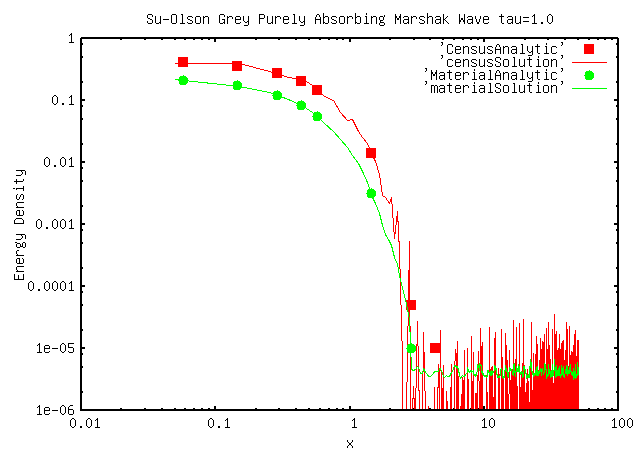
\includegraphics[width=\imgwidth,height=\imgheight]{Grey_MW_No_DF_L=50}}
		\end{picture}
		\caption{\label{fig:Grey_MW_No_DF_L=50} Normalized one dimensional grey solution compared to Su and Olson result[Su 1996] at $\tau=1.0$ with no scattering and no difference formulation. (Problem 1.1)}
		\end{minipage} \hfill
	\end{center}
\end{figure}

 	Figure \ref{fig:Grey_MW_No_DF_L=50} demonstrates the results obtained from the optimized grey IMD code. In this figure ``censusSolution'' denotes the photon energy density as determined by the IMD method, ``CensusAnalytic'' represents the semi-analytic benchmark results from Su and Olson, ``materialSolution'' denotes the material energy density calculated via the IMD method and finally ``MaterialAnalytic'' is the semi-analytic material energy density benchmark results from Su and Olson.

	The results from the multigroup calculation of this test problem are shown in Figure \ref{fig:Grey_MG_MW_No_DF_L=50}.

\begin{figure}[htbp]
	\unitlength1in
	\begin{center}
		\begin{minipage}[t]{6in}
		\centering
		\begin{picture}(\width,\height)
	                {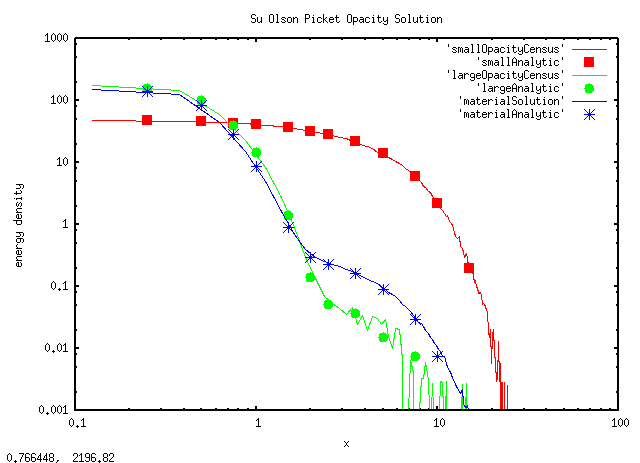
\includegraphics[width=\imgwidth,height=\imgheight]{Grey_MG_MW_No_DF_L=50}}
		\end{picture}
		\caption{\label{fig:Grey_MG_MW_No_DF_L=50} Grey IMD solution run with the multigroup IMD code compared to Su and Olson result[Su 1996]. (Problem 1.1)}
		\end{minipage} %\hfill
	\end{center}
\end{figure}

	Next, the effect of spatial (Problem 1.2a) and temporal (Problem 1.2b) refinement was investigated with the grey IMD code. This problem will be referred to as ``Problem 1.2''. Five versions of this test problem were run for each type of refinement. The spatial refinement was tested using the basic run settings defined in Table \ref{table:Problem1.2a}.  The different spatial refinements are listed in Table \ref{table:Problem1.2Spaital}.

\begin{table}[htbp]
	\begin{center}	
	\begin{tabular} {|c||c|c|c|} \hline
		\multicolumn{3}{|c|} {Problem 1.2 Parameters} \\ [0.5ex]\hline
		Parameter & Value  & Units \\ [0.5ex] \hline\hline
		{{Number of Cells}} 	& 120 	& N/A \\ \hline
		{{Number of Particles}} & 10000 	& N/A \\ \hline
		{{Length}} 		& 15 	& Mm \\ \hline
		{{Left Albedo}} 	& 0 	& N/A \\ \hline
		{{Right Albedo}} 	& 1 	& N/A \\ \hline
		{{Initial Material Temp.}} & 0.01 & K \\ \hline
		{{Material Density}} 	& 1.0 	& Kg/Mm \\ \hline
		{{Number Of Time Steps}}& 20 	& N/A \\ \hline
		{{Final Time [$\tau$]}} & 1.0 	& N/A \\ \hline
		{{Material Opacity}} 	& 1.0 	& 1/Mm \\ \hline
	\end{tabular}
	\caption{\label{table:Problem1.2a} Problem specifications used for Problem 1.2.}
	\end{center}
 \end{table}

\begin{table}[htbp]
	\begin{center}	
	\begin{tabular} {|c|c|} \hline
		\multicolumn{2}{|c|} {Problem 1.2a Spatial Refinements} \\ [0.5ex]\hline
		Number of Cells & Cell Size \\ [0.5ex] \hline\hline
		60  & 0.25  \\ \hline
		120 & 0.125	 \\ \hline
		240 & 0.0625	 \\ \hline
		480 & 0.03125	 \\ \hline
		960 & 0.015625  \\ \hline
	\end{tabular}
	\caption{\label{table:Problem1.2Spaital} Spatial refinements for Problem 1.2a}
	\end{center}
 \end{table}

\begin{figure}[htbp]
	\unitlength1in
	\begin{center}
		\begin{minipage}[t]{6in}
		\centering
		\begin{picture}(\width,\height)
	                {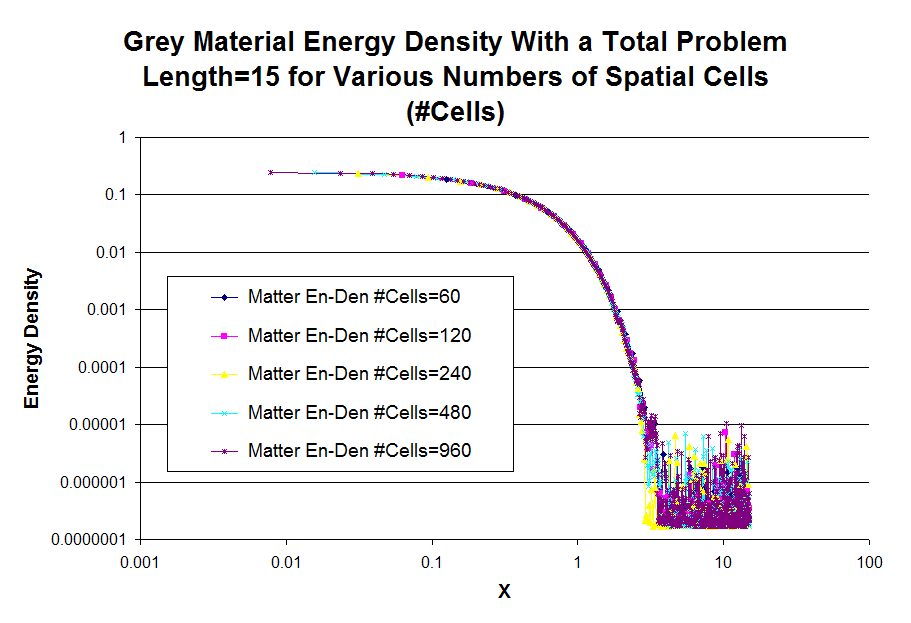
\includegraphics[width=\imgwidth,height=\imgheight]{G-Refine-Space}}
		\end{picture}
		\caption{\label{fig:Grey-Spatial-Refinment} Material energy densities from the grey IMD code with various cell sizes. (Problem 1.2a)}
		\end{minipage} %\hfill
	\end{center}
\end{figure}

	
	Figure \ref{fig:Grey-Spatial-Refinment} demonstrates the material energy density determined by the grey IMD code for various cell sizes. This shows that spatial refinement has very little relative effect on the shape of the material energy density.

	The temporal refinement for Problem 1.2 was performed using settings identical to those described in Table \ref{table:Problem1.2a}. Table \ref{table:Problem1.2Tempral} lists the five temporal refinements that were considered.

\begin{table}[htbp]
	\begin{center}	
	\begin{tabular} {|c|c|} \hline
		\multicolumn{2}{|c|} {Problem 1.2b Temporal Refinements} \\ [0.5ex]\hline
		Number of Time Steps & Time Step Size $\Delta{\tau}$ \\ [0.5ex] \hline\hline
		 10  & 0.1      \\ \hline
		 120 & 0.05     \\ \hline
		 240 & 0.025    \\ \hline
		 480 & 0.0125   \\ \hline
		 960 & 0.00625  \\ \hline
	\end{tabular}
	\caption{\label{table:Problem1.2Tempral} Temporal refinements for Problem 1.2b}
	\end{center}
 \end{table}

\begin{figure}[htbp]
	\unitlength1in
	\begin{center}
		\begin{minipage}[t]{6in}
		\centering
		\begin{picture}(\width,\height)
	                {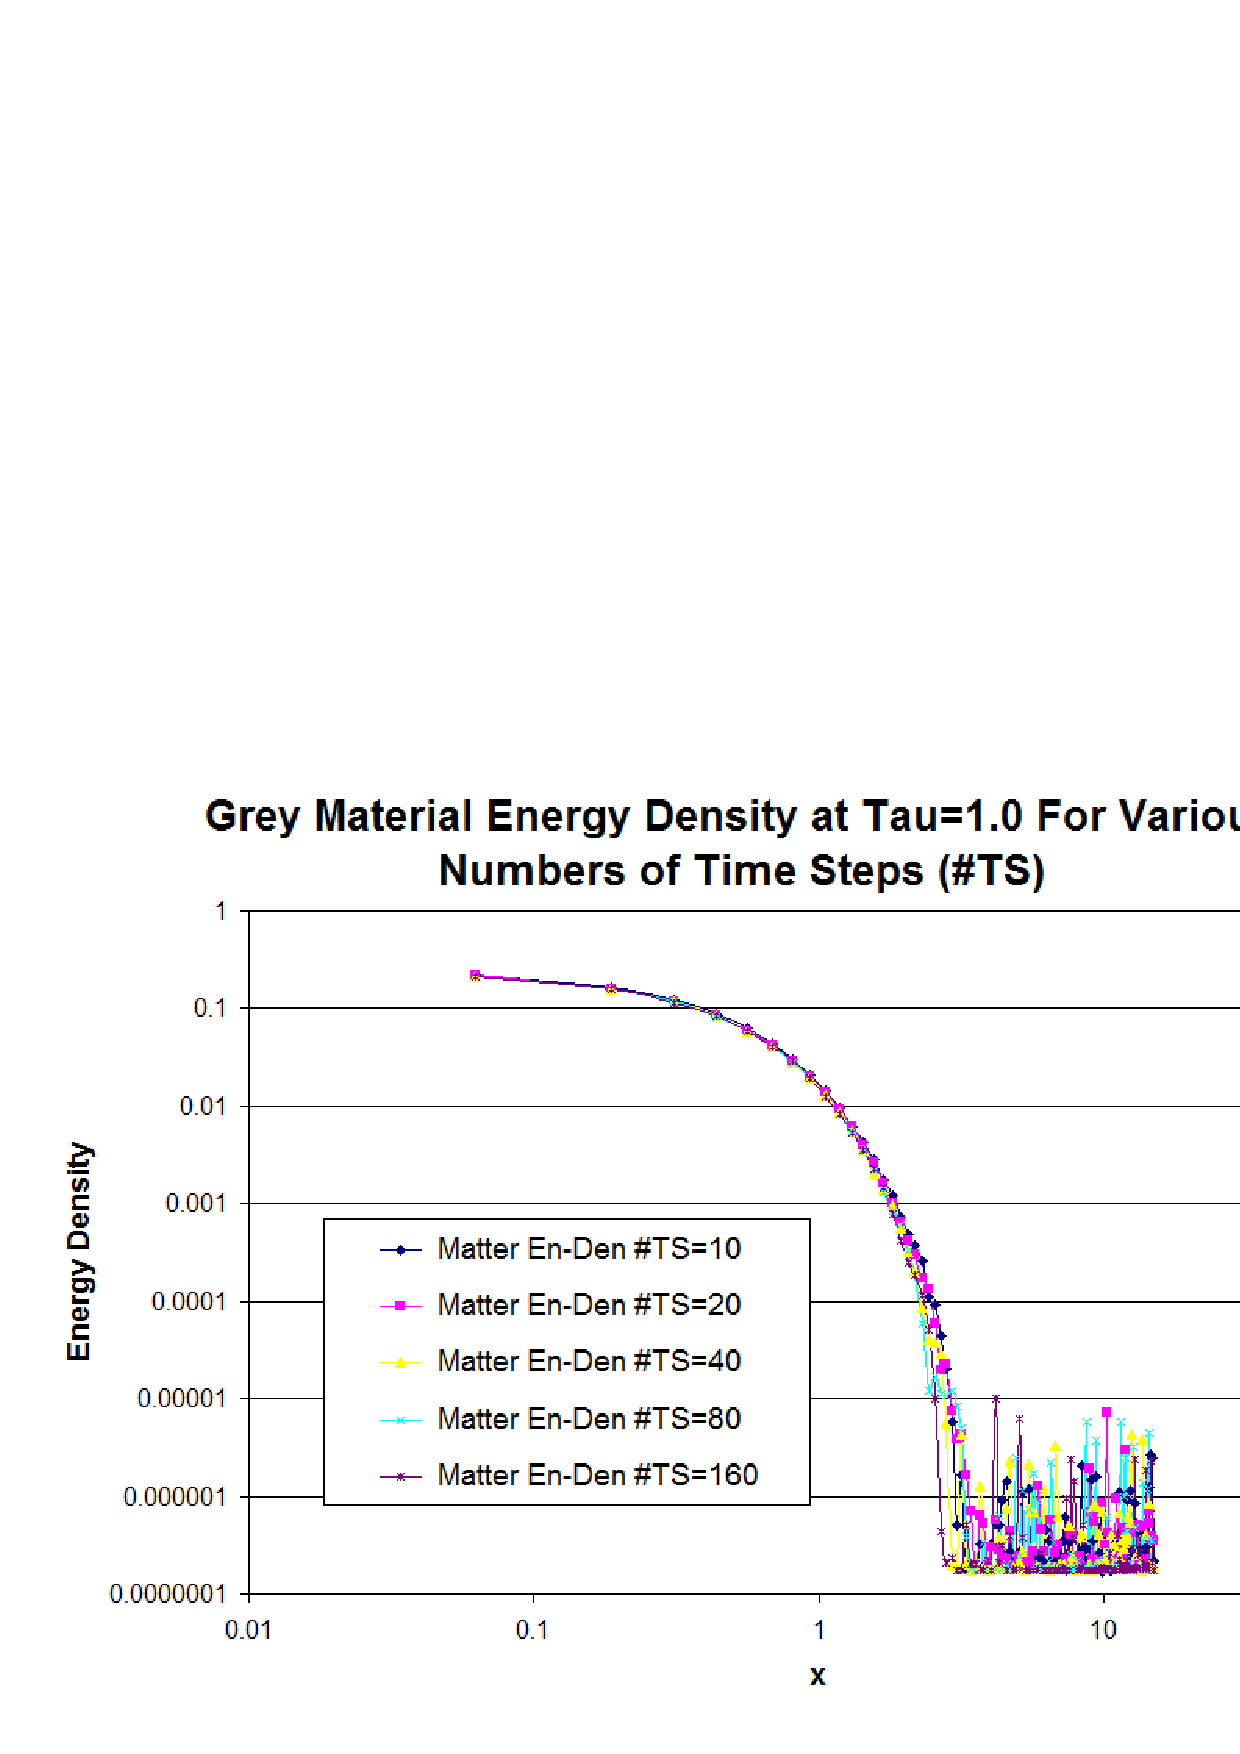
\includegraphics[width=\imgwidth,height=\imgheight]{G-Refine-time}}
		\end{picture}
		\caption{\label{fig:Grey-Tempral-Refinment1} Material energy densities from the grey IMD code with various time step sizes. (Problem 1.2b)}
		\end{minipage} %\hfill
	\end{center}
\end{figure}

\begin{figure}[htbp]
	\unitlength1in
	\begin{center}
		\begin{minipage}[t]{6in}
		\centering
		\begin{picture}(\width,\height)
	                {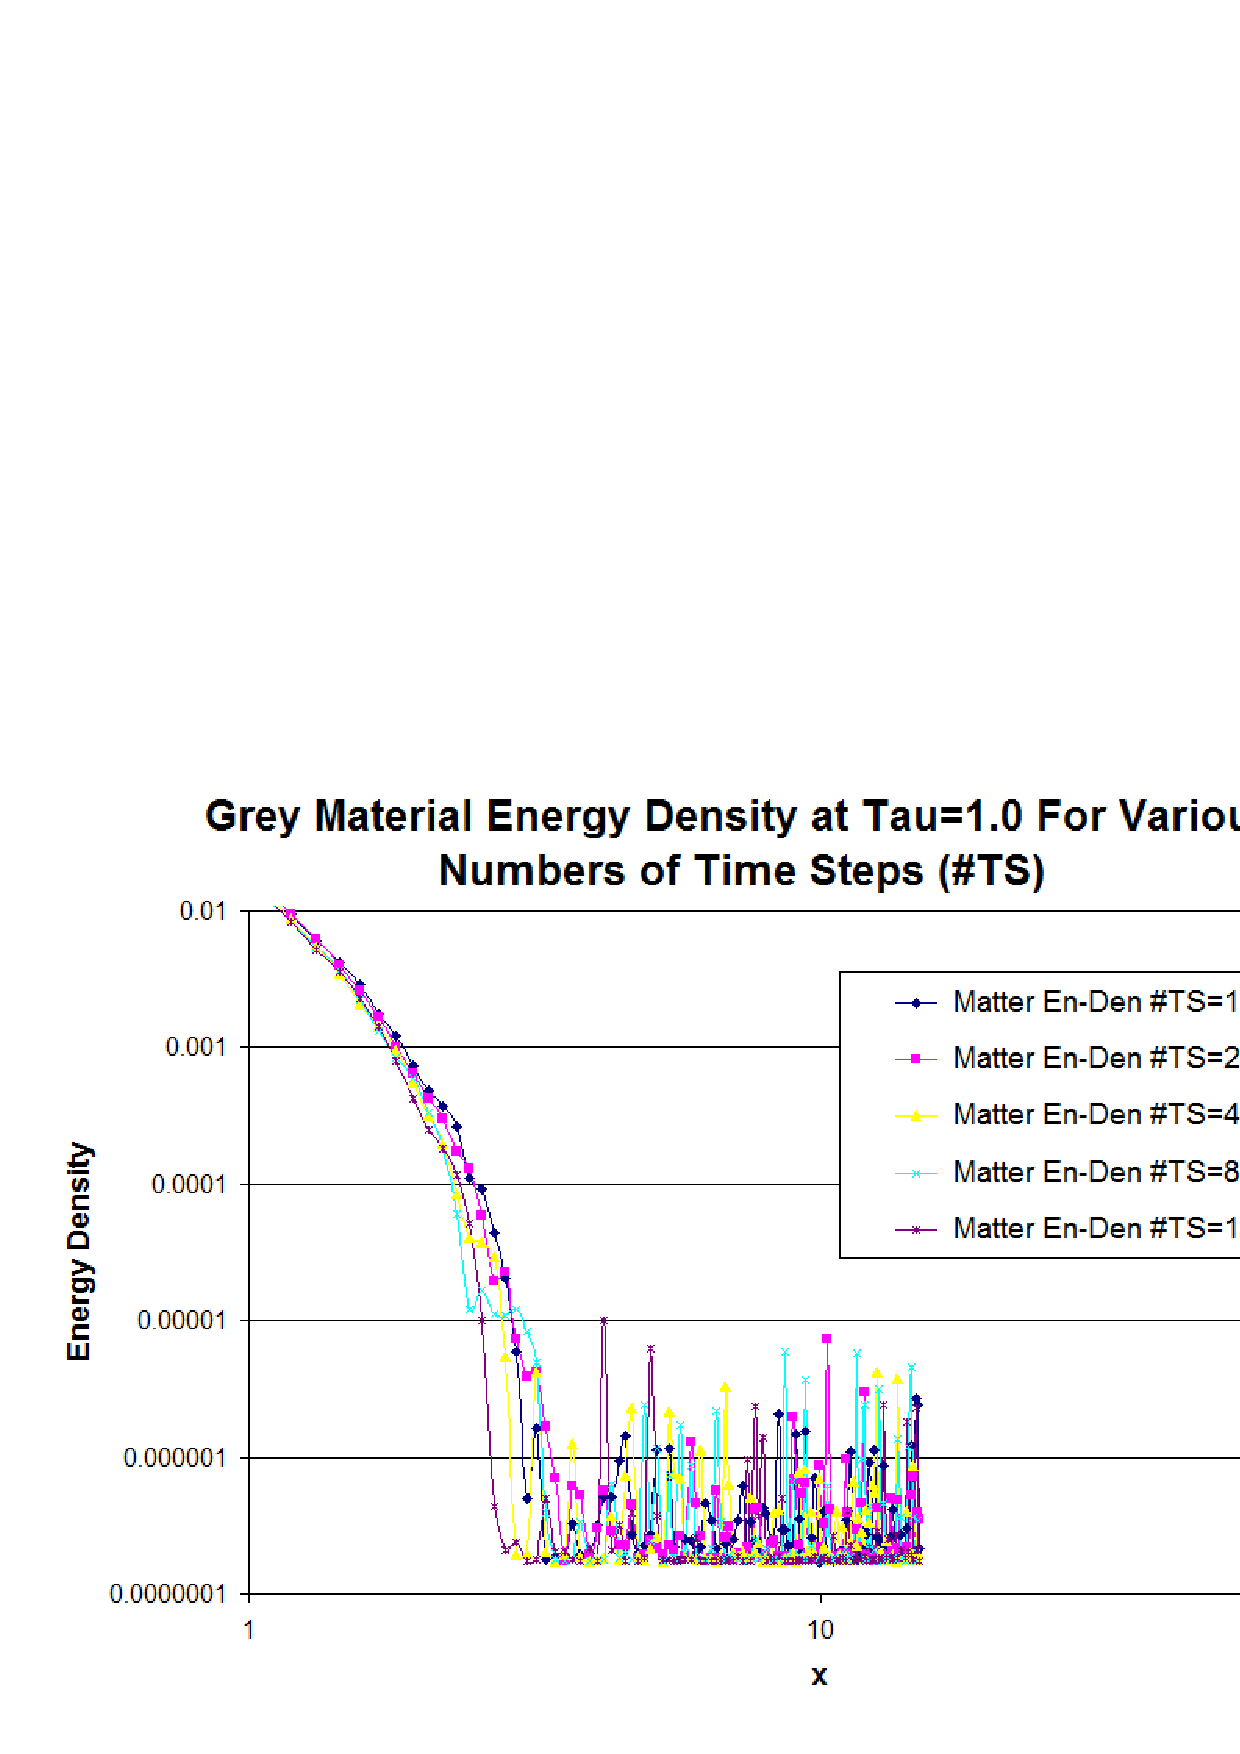
\includegraphics[width=\imgwidth,height=\imgheight]{G-Refine-time2}}
		\end{picture}
		\caption{\label{fig:Grey-Tempral-Refinment2} A closer look at the leading edge of the Marshak wave material energy densities from the grey IMD code with various time step sizes. (Problem 1.2b)}
		\end{minipage} %\hfill
	\end{center}
\end{figure}

	Figures \ref{fig:Grey-Tempral-Refinment1} and \ref{fig:Grey-Tempral-Refinment2} show that the degree of temporal refinement has a greater effect on the numerical solution than the degree of the spatial refinement. This is paticularly true at the leading edge of the Marshak wave.
%==================%
% SubSubSection:   %
%    Grey Without the Difference Formulation %
%==================%
\subsubsection{Grey with the Difference Formulation}
\label{sec:Grey_w/df}

	In Problem 1.2, the Su and Olson grey benchmark result is simulated using the optimized grey IMD code and the difference formulation. In this case, the difference formulation temperature was chosen to be the material temperature in the associated cell. This problem has parameters identical to those of Problem 1.1 (see Table \ref{table:Problem1.1}).

\begin{figure}[htbp]
	\unitlength1in
	\begin{center}
		\begin{minipage}[t]{6in}
		\centering
		\begin{picture}(\width,\height)
	                {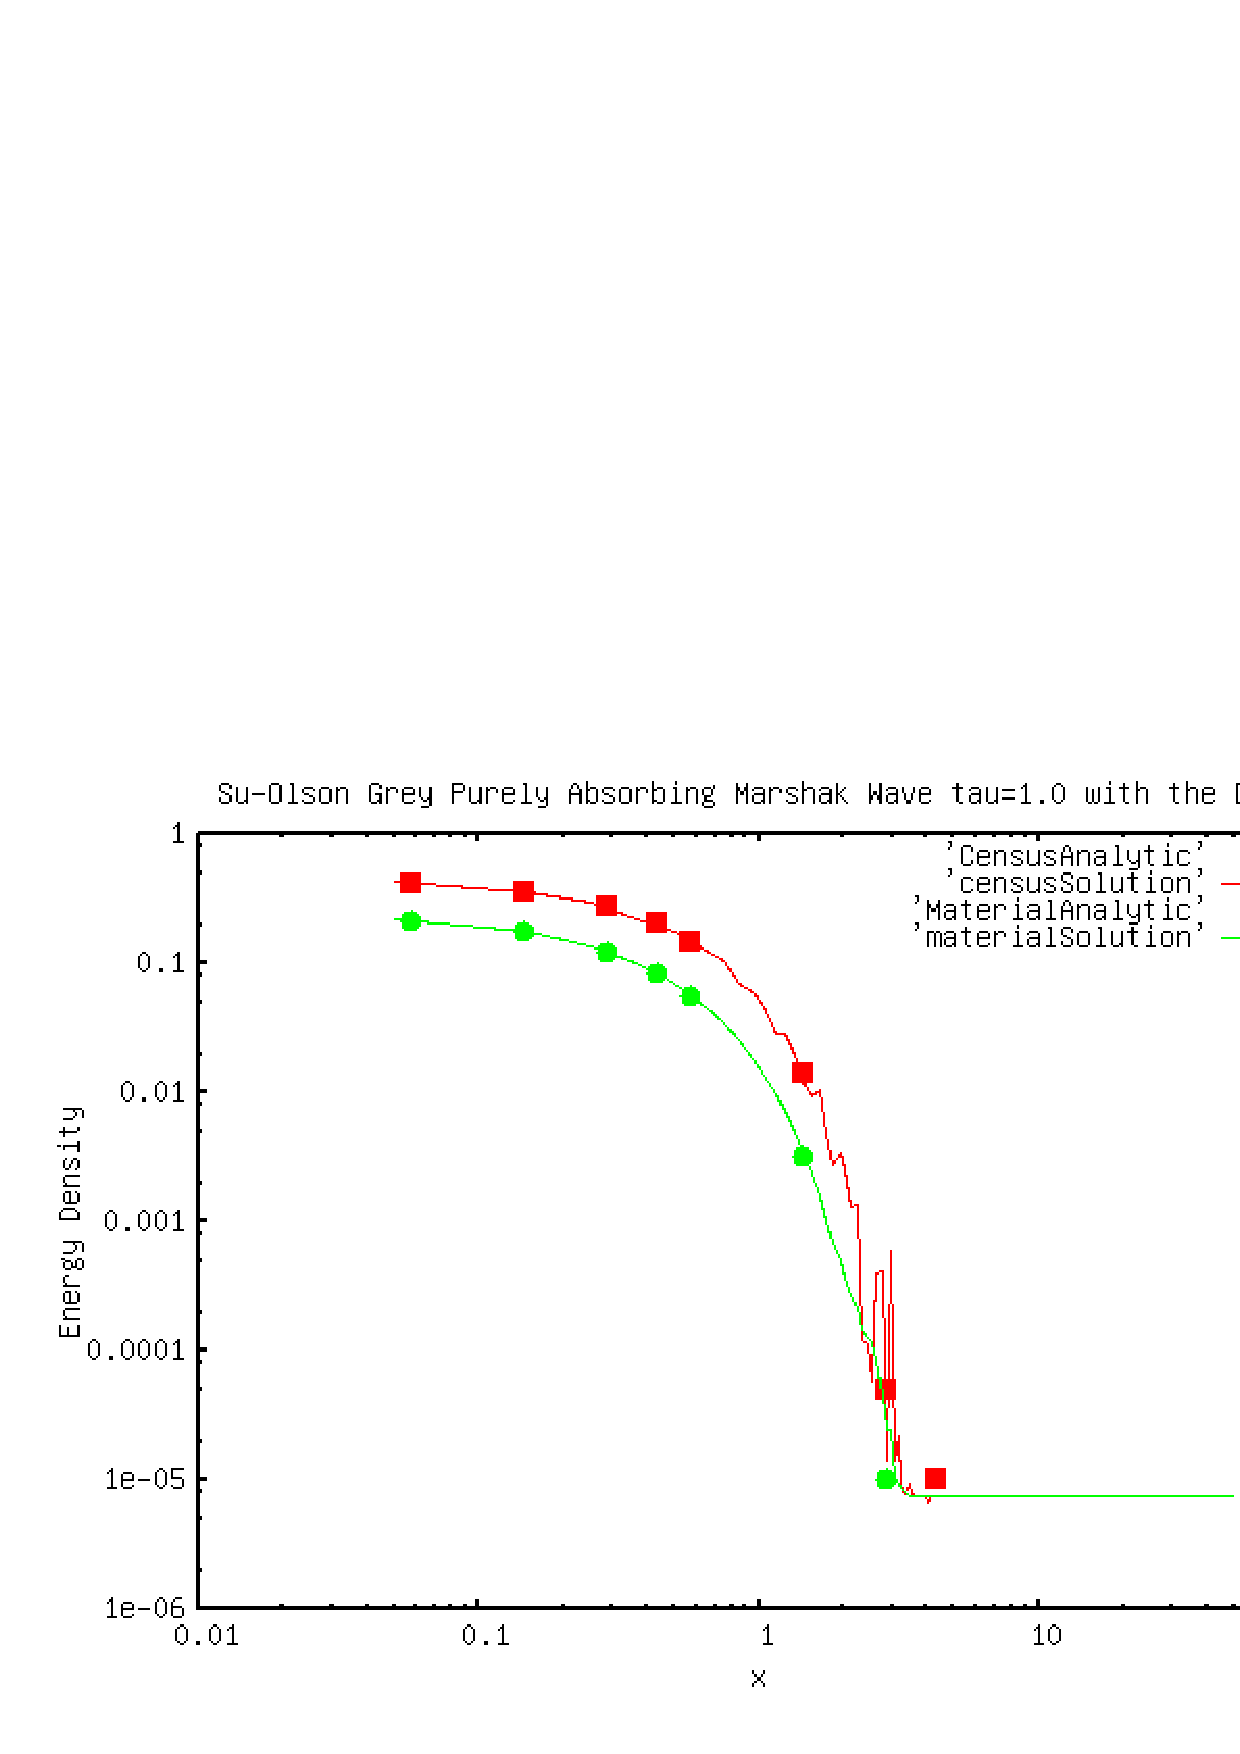
\includegraphics[width=\imgwidth,height=\imgheight]{Grey_MW_DF_L=50}}
		\end{picture}
		\caption{\label{fig:Grey_MW_DF_L=50} Normalized one dimensional grey solution  with the difference formulation compared to Su and Olson result[Su 1996] at $\tau=1.0$ with no scattering. (Problem 1.1)}
		\end{minipage} %\hfill
	\end{center}
\end{figure}

	The difference between figures \ref{fig:Grey_MW_DF_L=50} and \ref{fig:Grey_MW_No_DF_L=50} show that the difference formulation yields a significant reduction in the variance.

\belowSubSecSkip

%=====================================================================%
% SubSection:                        	                              %
%     Results: Markov-Markov Mixing Statistics - Vacuum Boundaries %
%=====================================================================%
\subsection{Frequency Dependent Implicit Monte Carlo Diffusion}
\label{sec:Results-MM-V}

\noindent
	\indent This section contains the results of test problems solved using the frequency dependent IMD method. This includes an exploration of frequency dependent systems with and without the difference formulation. The majority of the simulated results are compared against the Su and Olson non-grey Marshak wave semi-analytic benchmark with a picket fence opacity. The stability and accuracy of the method are investigated as both the number of time steps and the number of cells is varied. 

%==================%
% SubSubSection:   %
%    Grey Without the Difference Formulation %
%==================%
\subsubsection{Frequency Dependent IMD without the Difference Formulation}
\label{sec:Grey_w/out_df}

	The next problem is the Su and Olson non-grey benchmark result with a picket fence opacity defined such that: the bins are logarithmically spaced in frequency, even frequency bins have a large opacity, and odd frequency bins have a small opacity. The opacities are chosen such that the Planck opacity, defined by equation \ref{PlanckOpacity2}, is equal to one[Su 1999]. The opacities chosen for this work are shown in Table \ref{table:opacities}

\begin{table}[htbp]
	\begin{center}	
	\begin{tabular} {|c||c|} \hline
		\multicolumn{2}{|c|} {Picket Fence Opacities} \\ [0.5ex]\hline
		Number of Time Steps & Time Step Size $\Delta{\tau}$ \\ [0.5ex] \hline\hline
		 Small Opacity  & ${2\over{101}}$      \\ \hline
		 Large Opacity  & ${200\over{101}}$      \\ \hline
	\end{tabular}
	\caption{\label{table:opacities} Opacities used to construct the opacity distribution for the frequency dependent IMD results.}
	\end{center}
 \end{table}

	The remainder of the specifications for this problem (Problem 3.1) are listed in Table \ref{table:Problem2.1}.

\begin{table}[htbp]
	\begin{center}	
	\begin{tabular} {|c||c|c|c|} \hline
		\multicolumn{3}{|c|} {Problem 3.1 Parameters} \\ [0.5ex]\hline
		Parameter & Value  & Units \\ [0.5ex] \hline\hline
		{{Number of Cells}} 	& 120 	& N/A \\ \hline
		{{Number of Particles}} & 400000 & N/A \\ \hline
		{{Length}} 		& 15 	& Mm \\ \hline
		{{Left Albedo}} 	& 1 	& N/A \\ \hline
		{{Right Albedo}} 	& 1 	& N/A \\ \hline
		{{Initial Material Temp.}} & 0.01 & K \\ \hline
		{{Material Density}} 	& 1.0 	& Kg/Mm \\ \hline
		{{Number Of Time Steps}}& 40 	& N/A \\ \hline
		{{Final Time [$\tau$]}} 	& 1.0 	& N/A \\ \hline
		{{Small Opacity}} 	& ${2\over{101}}$  & 1/Mm \\ \hline
		{{Large Opacity}} 	& ${200\over{101}}$  & 1/Mm \\ \hline
	\end{tabular}
	\caption{\label{table:Problem2.1} Problem specifications used for the Su and Olson purely absorbing grey Marshak wave problem at $\tau=1.0$ (Problem 3.1).}
	\end{center}
 \end{table}

\begin{figure}[htbp]
	\unitlength1in
	\begin{center}
		\begin{minipage}[t]{6in}
		\centering
		\begin{picture}(\width,\height)
	                {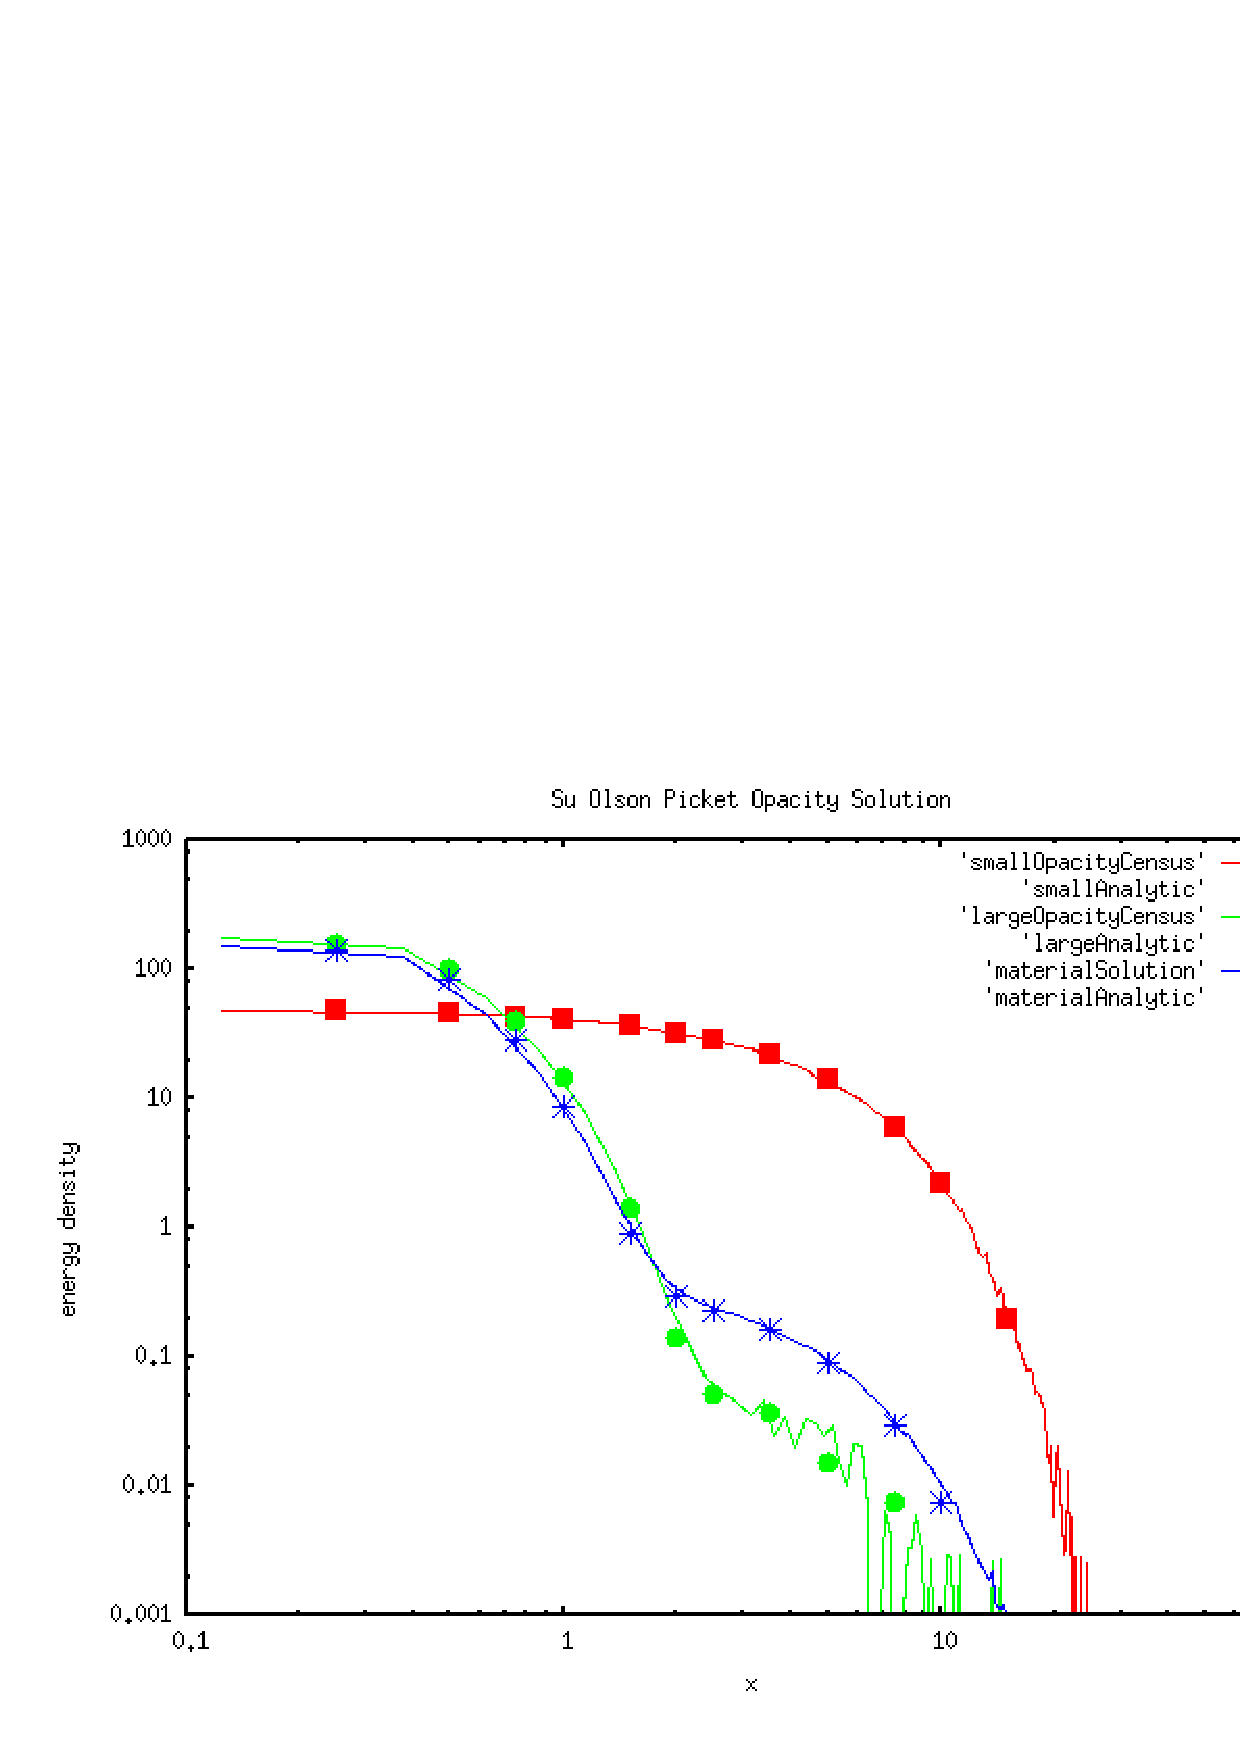
\includegraphics[width=\imgwidth,height=\imgheight]{NG-SO}}
		\end{picture}
		\caption{\label{fig:NG-SO} Normalized one dimensional frequency dependent solution compared to Su and Olson result[Su 1999] at $\tau=1.0$ with no difference formulation. (Problem 3.1)}
		\end{minipage} %\hfill
	\end{center}
\end{figure}

 	Figure \ref{fig:NG-SO} shows that the IMD code can accurately reproduce multigroup solutions. Here ``smallOpacityCensus'', ``largeOpacityCensus'', and ``materialSolution'' refer to the photon energy density for the small opacity, large opacity, and the material energy density respectively, as calculated by the multigroup IMD code. The Su and Olson semi-analytic result for the small opacity photon energy density, large opacity photon energy density, and material energy density are labeled as ``smallAnalytic'', ``largeAnalytic'', and ``materialAnalytic''.

	The effect of spatial (Problem 3.2a) and temporal (Problem 3.2b) resolution on the frequency dependent IMD method was tested with the parameters defined in Table \ref{table:Problem3.2}. The spatial and temporal resolution used for these problems are shown in Tables \ref{table:Problem1.2Spaital} and \ref{table:Problem1.2Tempral} respectively.

\begin{table}[htbp]
	\begin{center}	
	\begin{tabular} {|c||c|c|c|} \hline
		\multicolumn{3}{|c|} {Problem 3.2 Parameters} \\ [0.5ex]\hline
		Parameter & Value  & Units \\ [0.5ex] \hline\hline
		{{Number of Cells}} 	& 120 	& N/A \\ \hline
		{{Number of Particles}} & 10000 & N/A \\ \hline
		{{Length}} 		& 15 	& Mm \\ \hline
		{{Left Albedo}} 	& 1 	& N/A \\ \hline
		{{Right Albedo}} 	& 1 	& N/A \\ \hline
		{{Initial Material Temp.}} & 0.01 & K \\ \hline
		{{Material Density}} 	& 1.0 	& Kg/Mm \\ \hline
		{{Number Of Time Steps}}& 20 	& N/A \\ \hline
		{{Final Time [$\tau$]}} 	& 1.0 	& N/A \\ \hline
		{{Small Opacity}} 	& ${2\over{101}}$  & 1/Mm \\ \hline
		{{Large Opacity}} 	& ${200\over{101}}$  & 1/Mm \\ \hline
		{{Number of Groups}} 	& 1000  & 1/Mm \\ \hline	
	\end{tabular}
	\caption{\label{table:Problem3.2} Problem specifications used for the frequency dependent temporal and spatial refinement. (Problem 3.2)}
	\end{center}
 \end{table}

\begin{figure}[htbp]
	\unitlength1in
	\begin{center}
		\begin{minipage}[t]{6in}
		\centering
		\begin{picture}(\width,\height)
	                {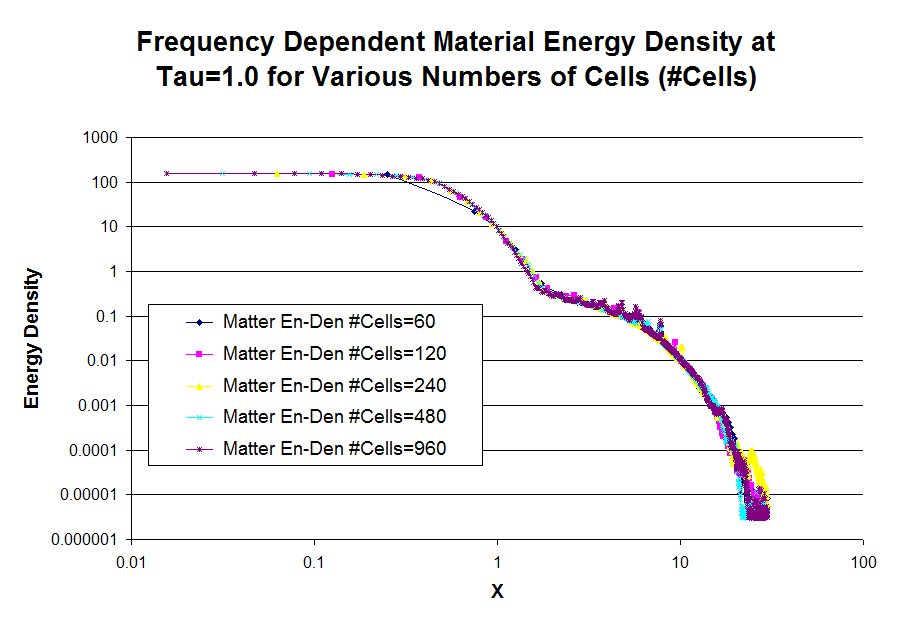
\includegraphics[width=\imgwidth,height=\imgheight]{NG-Refine-Space}}
		\end{picture}
		\caption{\label{fig:NG-Refine-Space} Frequency dependent IMD solution for various cell sizes. (Problem 3.2a)}
		\end{minipage} %\hfill
	\end{center}
\end{figure}

	Figure \ref{fig:NG-Refine-Space} shows the solution to the frequency dependent IMD method with the various spatial refinements. The solution is relatively insensitive to the choice of spatial cell size.

\begin{figure}[htbp]
	\unitlength1in
	\begin{center}
		\begin{minipage}[t]{6in}
		\centering
		\begin{picture}(\width,\height)
	                {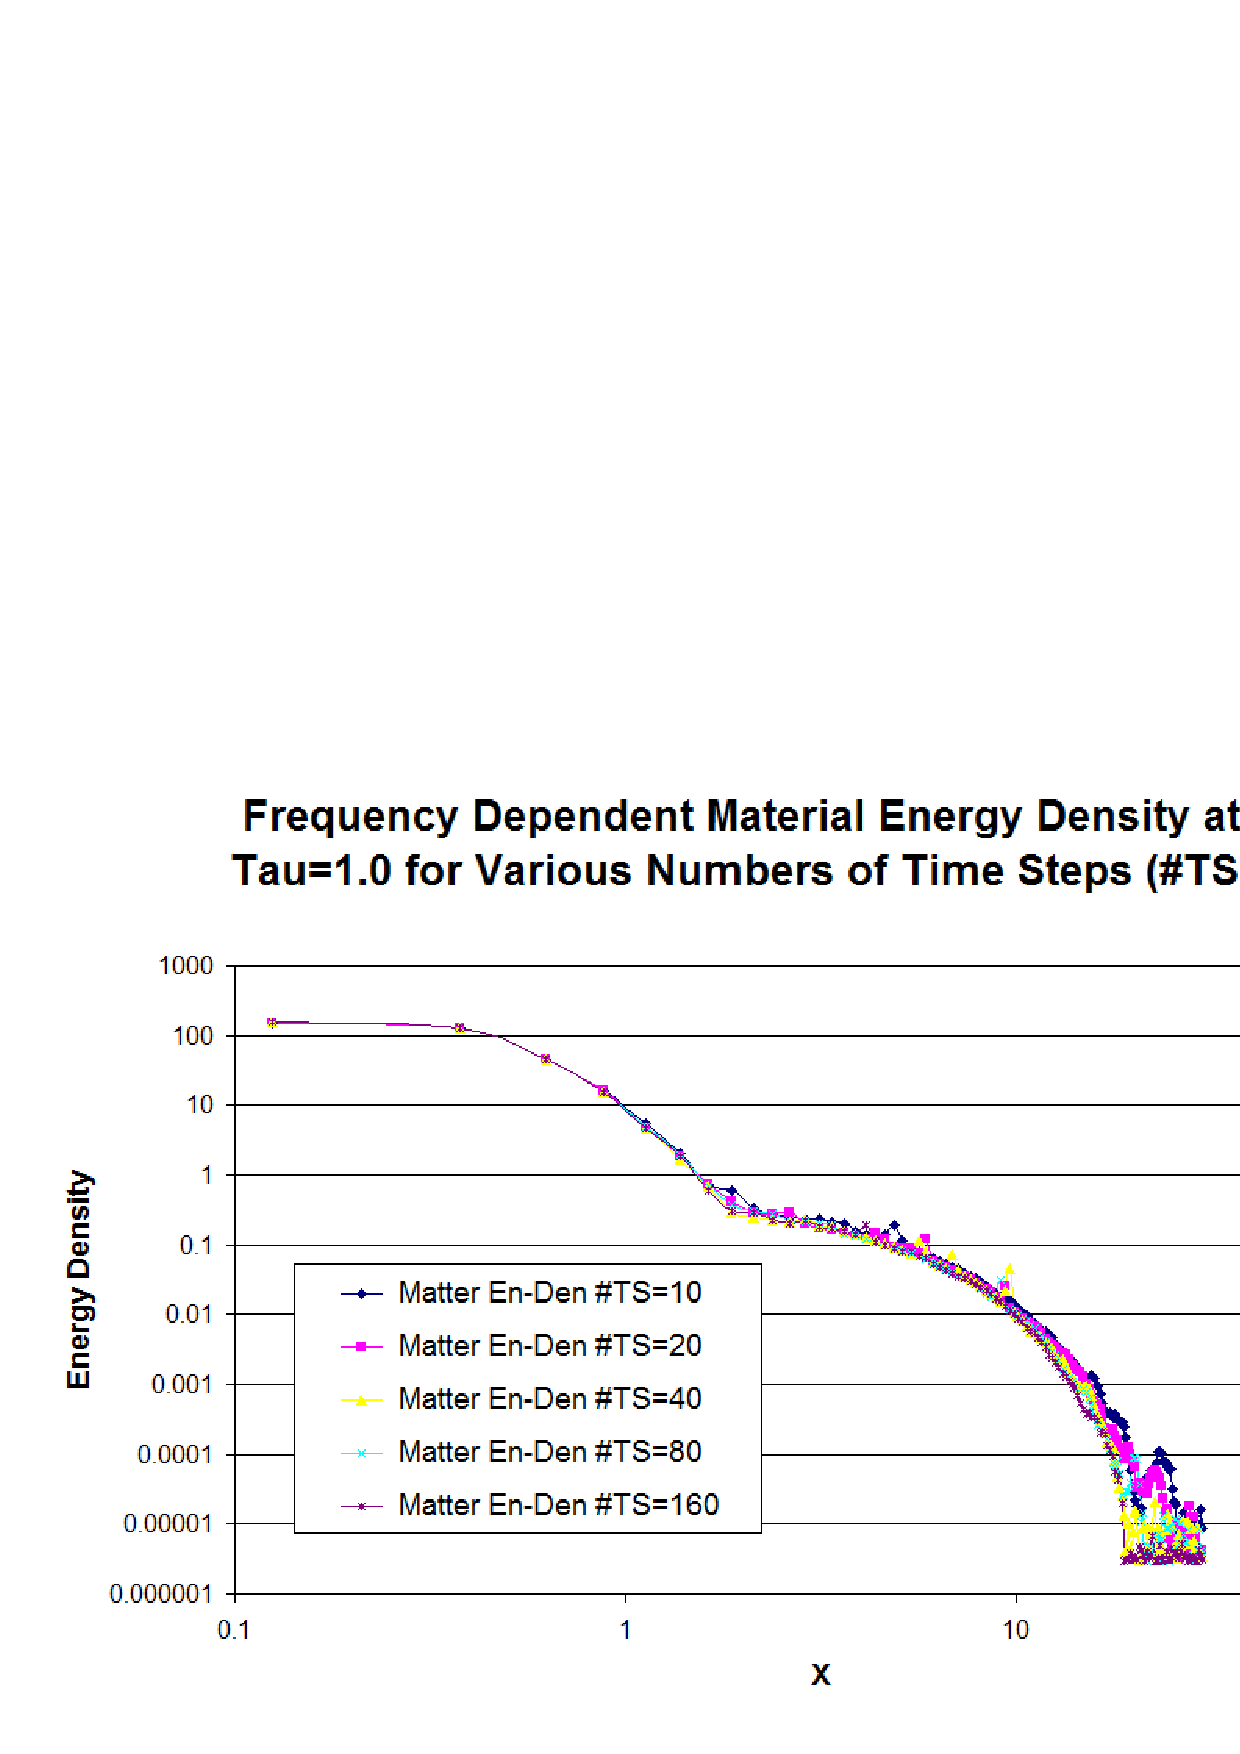
\includegraphics[width=\imgwidth,height=\imgheight]{NG-Refine-time1}}
		\end{picture}
		\caption{\label{fig:NG-Refine-time1} Frequency dependent IMD solution for various time step sizes. (Problem 3.2b)}
		\end{minipage} %\hfill
	\end{center}
\end{figure}

\begin{figure}[htbp]
	\unitlength1in
	\begin{center}
		\begin{minipage}[t]{6in}
		\centering
		\begin{picture}(\width,\height)
	                {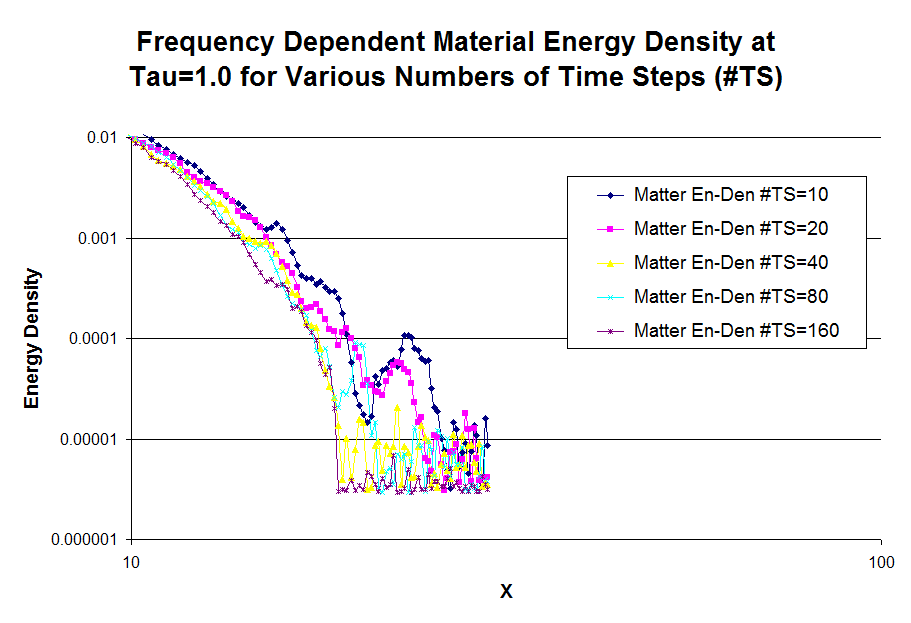
\includegraphics[width=\imgwidth,height=\imgheight]{NG-Refine-time2}}
		\end{picture}
		\caption{\label{fig:NG-Refine-time2} A closer view of the frequency dependent IMD solution for various time step sizes at the head of the Marshak wave. (Problem 3.2b)}
		\end{minipage} %\hfill
	\end{center}
\end{figure}

	Figures \ref{fig:NG-Refine-time1} and \ref{fig:NG-Refine-time2} show the dependence on the time step size. The penetration distance of the Marshak wave is influenced by the time step size. 

	The group refinement on the material energy density and the effect of frequency group calculation time was also investigated. This set of problems has the specifications in Table \ref{table:Problem3.3} with several choices of group structures: 1000 groups, 2000 groups, 4000 groups, 8000 groups, and 16000 groups. 

\begin{table}[htbp]
	\begin{center}	
	\begin{tabular} {|c||c|c|c|} \hline
		\multicolumn{3}{|c|} {Problem 3.3 Parameters} \\ [0.5ex]\hline
		Parameter & Value  & Units \\ [0.5ex] \hline\hline
		{{Number of Cells}} 	& 120 	& N/A \\ \hline
		{{Number of Particles}} & 10000 & N/A \\ \hline
		{{Length}} 		& 30 	& Mm \\ \hline
		{{Left Albedo}} 	& 1 	& N/A \\ \hline
		{{Right Albedo}} 	& 1 	& N/A \\ \hline
		{{Initial Material Temp.}} & 0.01 & K \\ \hline
		{{Material Density}} 	& 1.0 	& Kg/Mm \\ \hline
		{{Number Of Time Steps}}& 20 	& N/A \\ \hline
		{{Final Time [$\tau$]}} 	& 1.0 	& N/A \\ \hline
		{{Small Opacity}} 	& ${2\over{101}}$  & 1/Mm \\ \hline
		{{Large Opacity}} 	& ${200\over{101}}$  & 1/Mm \\ \hline
		{{Number of Groups}} 	& 1000  & 1/Mm \\ \hline	
	\end{tabular}
	\caption{\label{table:Problem3.3} Problem specifications used for the frequency dependent IMD with various numbers of groups. (Problem 3.3)}
	\end{center}
 \end{table}

\begin{figure}[htbp]
	\unitlength1in
	\begin{center}
		\begin{minipage}[t]{6in}
		\centering
		\begin{picture}(\width,\height)
	                {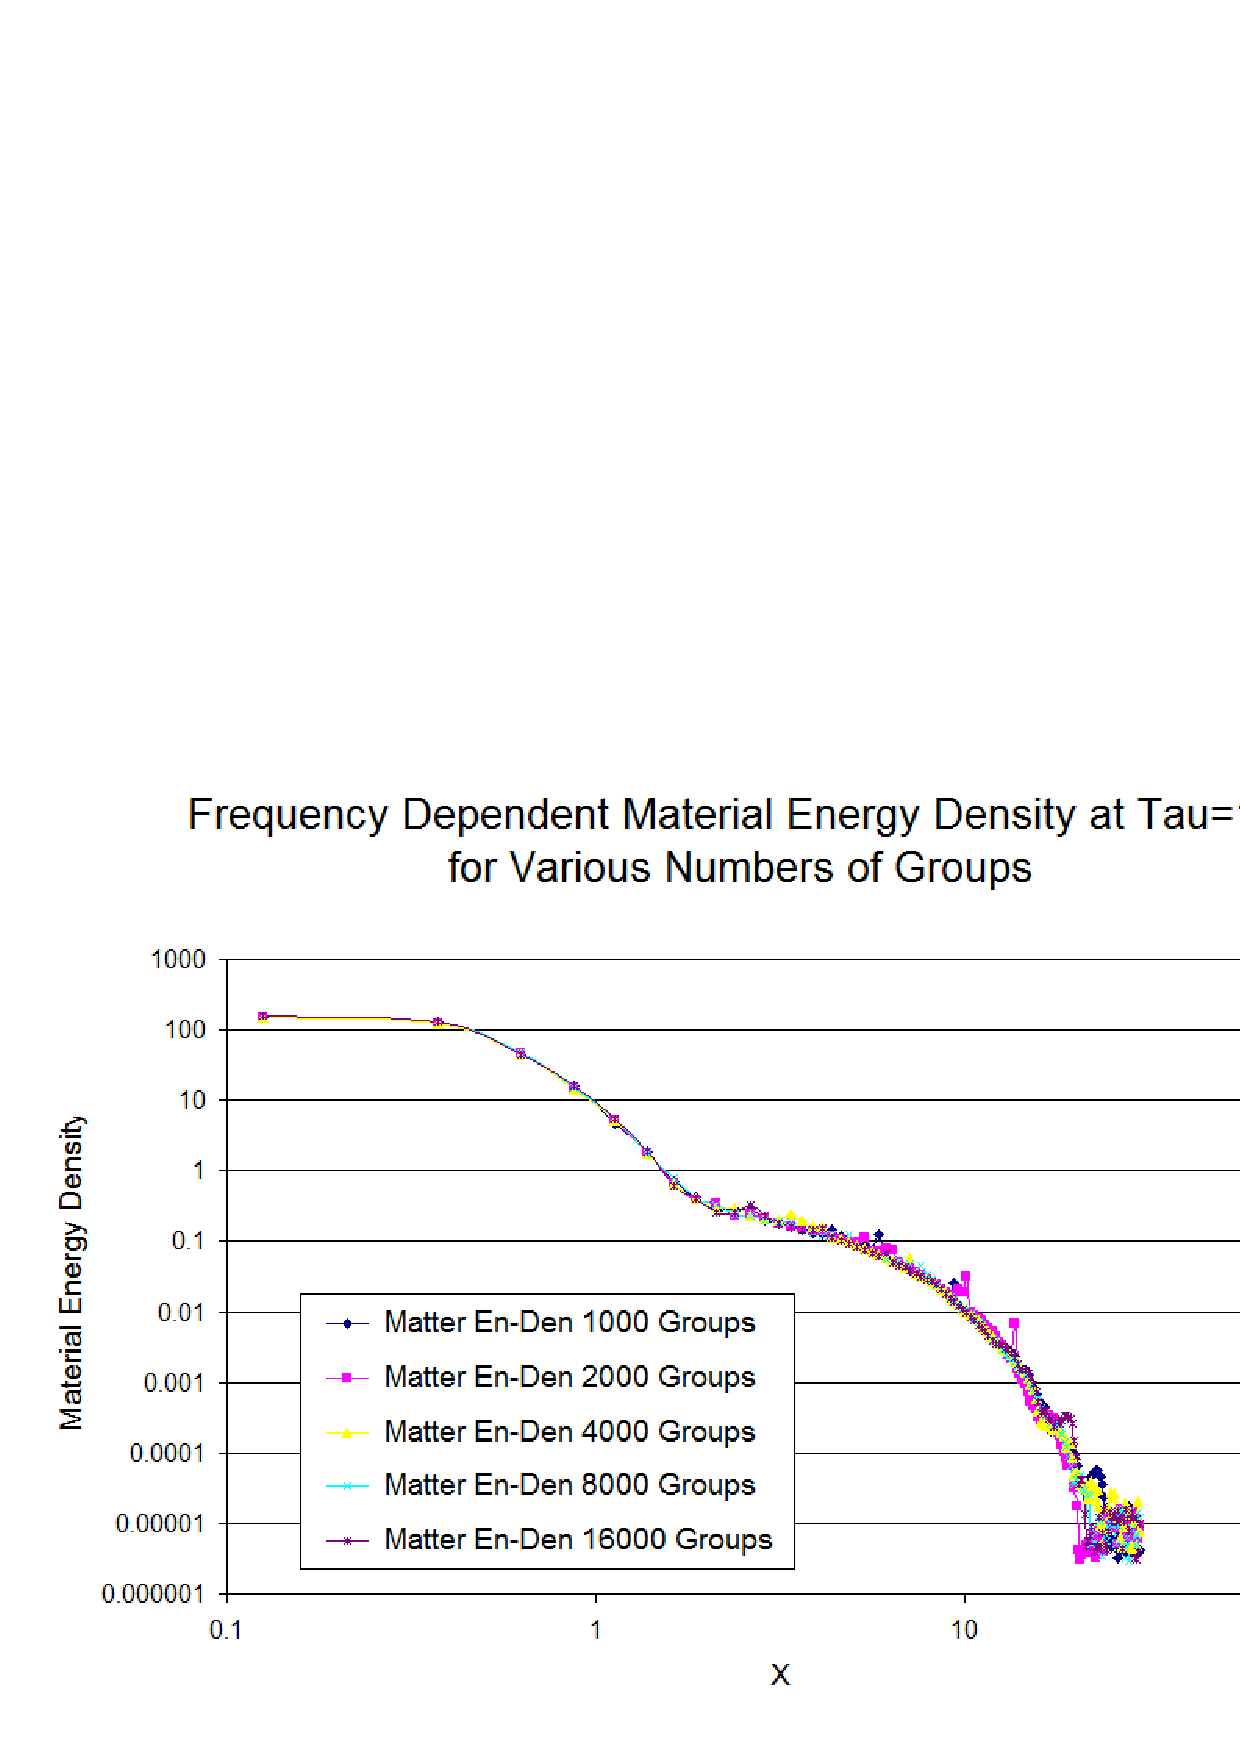
\includegraphics[width=\imgwidth,height=\imgheight]{NG-MG}}
		\end{picture}
		\caption{\label{fig:NG-MG} The material energy density determined by the frequency dependent IMD method for various numbers of groups. (Problem 3.3)}
		\end{minipage} %\hfill
	\end{center}
\end{figure}

\begin{figure}[htbp]
	\unitlength1in
	\begin{center}
		\begin{minipage}[t]{6in}
		\centering
		\begin{picture}(\width,\height)
	                {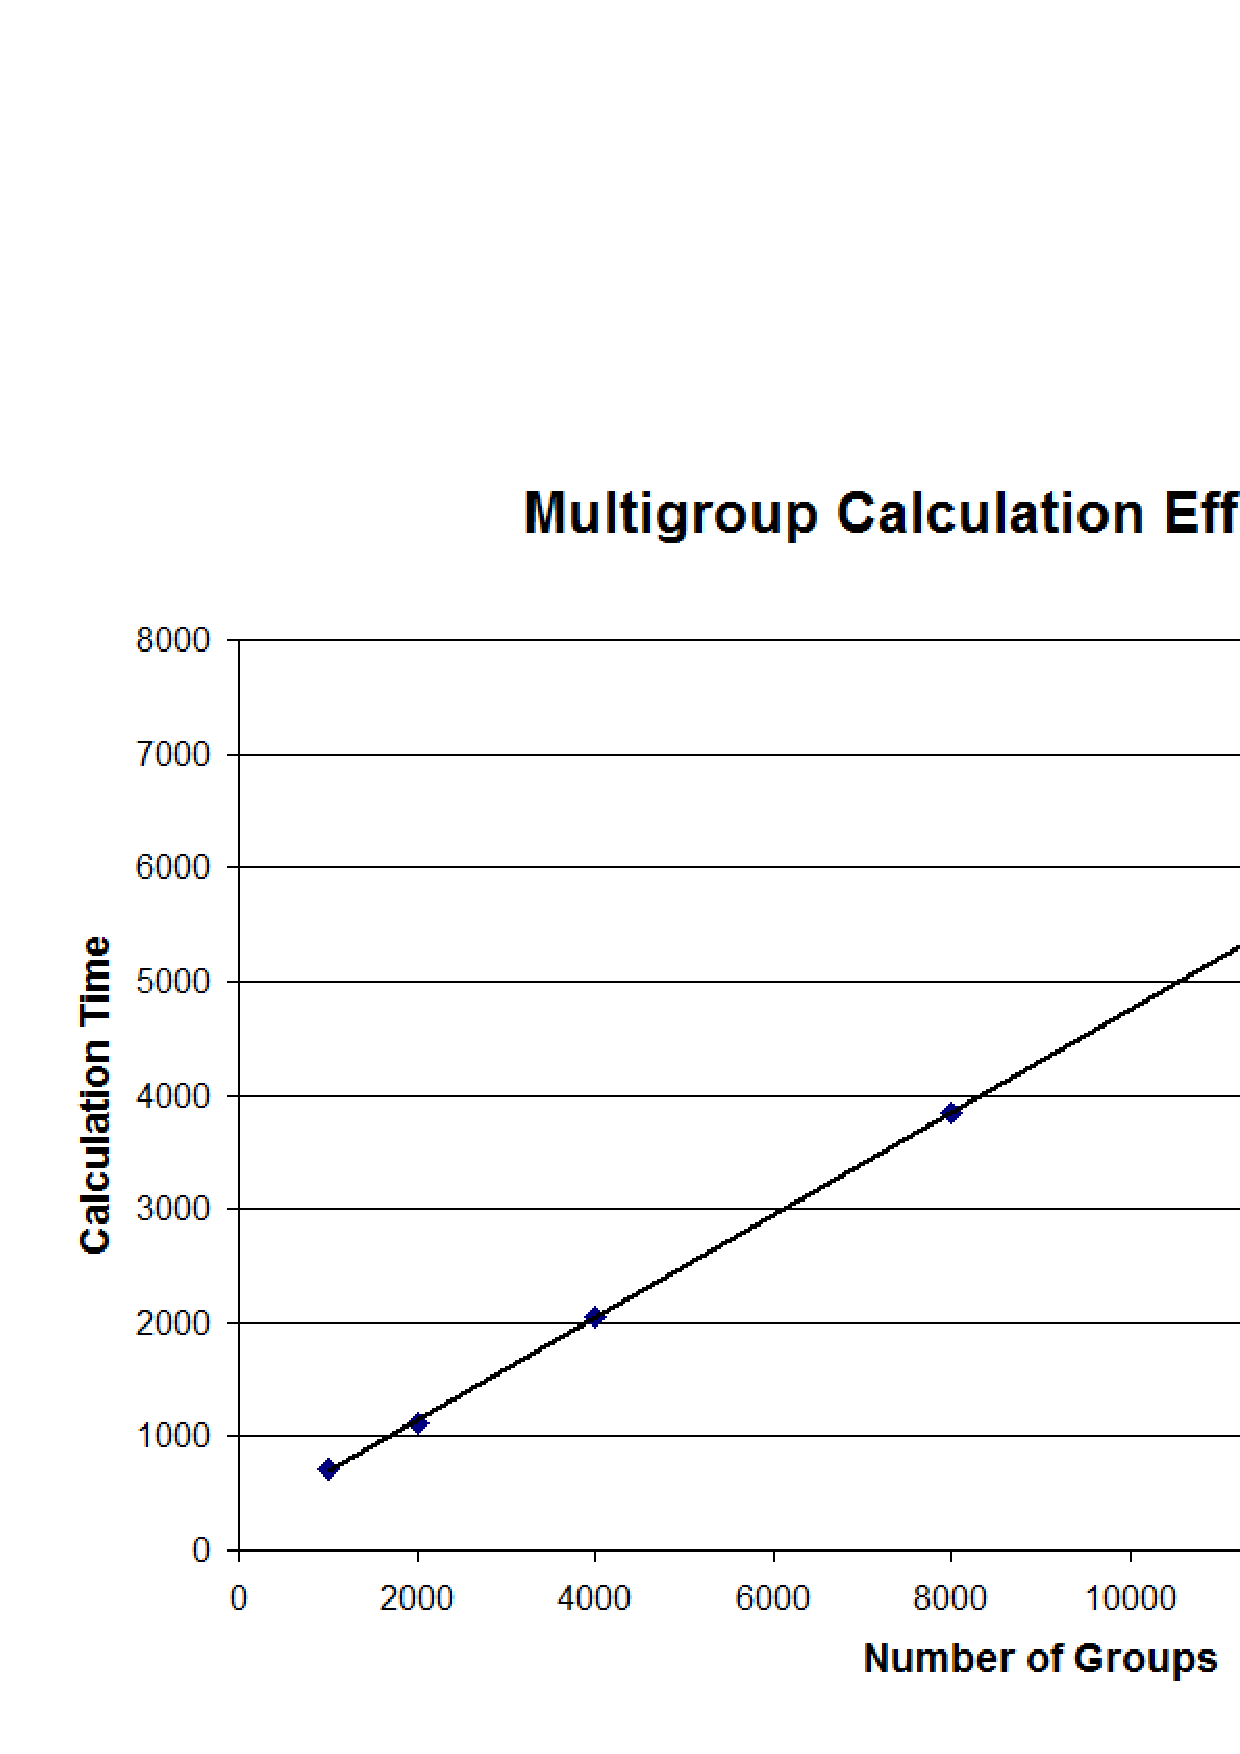
\includegraphics[width=\imgwidth,height=\imgheight]{MG_Calc_Efficiency}}
		\end{picture}
		\caption{\label{fig:MG-Calc-Efficiency} Computational cost as a function of number of groups used in the calculation (Problem 3.3)}
		\end{minipage} %\hfill
	\end{center}
\end{figure}

	The material energy density determined by the multigroup IMD method for various numbers of groups is shown in Figure \ref{fig:NG-MG}. Figure \ref{fig:MG-Calc-Efficiency} shows the computational cost as a function of numbers of groups used for the calculation.


%==================%5s
% SubSubSection:   %
%    Grey Without the Difference Formulation %
%==================%
\subsubsection{Frequency Dependent IMD with the Difference Formulation}
\label{sec:Grey_w/df}

	This section will explore properties of the frequency dependent implementation of IMD with the difference formulation. We will generate three different solutions using the IMD code with the difference formulation and one without the difference formulation. The problem specifications are listed in Table \ref{table:Problem4.1}. This problem will be referred to as ``Problem 4.1''.

\begin{table}[htbp]
	\begin{center}	
	\begin{tabular} {|c||c|c|c|} \hline
		\multicolumn{3}{|c|} {Problem 4.1 Parameters} \\ [0.5ex]\hline
		Parameter & Value  & Units \\ [0.5ex] \hline\hline
		{{Number of Cells}} 	& 500 	& N/A \\ \hline
		{{Number of Particles}} & 10000 & N/A \\ \hline
		{{Length}} 		& 50 	& Mm \\ \hline
		{{Left Albedo}} 	& 1 	& N/A \\ \hline
		{{Right Albedo}} 	& 1 	& N/A \\ \hline
		{{Initial Material Temp.}} & 0.01 & K \\ \hline
		{{Material Density}} 	& 1.0 	& Kg/Mm \\ \hline
		{{Number Of Time Steps}}& 20 	& N/A \\ \hline
		{{Final Time [$\tau$]}} & 1.0 	& N/A \\ \hline
		{{Small Opacity}} 	& ${2\over{101}}$  & 1/Mm \\ \hline
		{{Large Opacity}} 	& ${200\over{101}}$  & 1/Mm \\ \hline
	\end{tabular}
	\caption{\label{table:Problem4.1} Problem specifications used for the frequency dependent difference formulation tests. (Problem 4.1)}
	\end{center}
 \end{table}

	The temperature distribution used in the difference formulation is a user described quantity. This termperature is varied such that it was a defined percentage of the current material temperature for the associated cell. The percentages used for these problems are listed in Table \ref{table:percent-Tm}. we are interested in the effect this choice has on computational cost of the method and the degree of variance reduction.

\begin{table}[htbp]
	\begin{center}	
	\begin{tabular} {|c||c|} \hline
		\multicolumn{2}{|c|} {Difference Formulation Temperatures for Problem 4.1} \\ [0.5ex]\hline
		Problem Realization & \% Material Temperature \\ [0.5ex] \hline\hline
		 Problem 4.1a  & 00.0 \%      \\ \hline
		 Problem 4.1b  & 10.0 \%      \\ \hline
		 Problem 4.1c  & 30.0 \%      \\ \hline
		 Problem 4.1d  & 50.0 \%      \\ \hline
	\end{tabular}
	\caption{\label{table:percent-Tm} The percentages of the material temperature used for the difference formulation temperature. (Problem 4.1)}
	\end{center}
 \end{table}
	 
\begin{figure}[htbp]
	\unitlength1in
	\begin{center}
		\begin{minipage}[t]{6in}
		\centering
		\begin{picture}(\width,\height)
	                {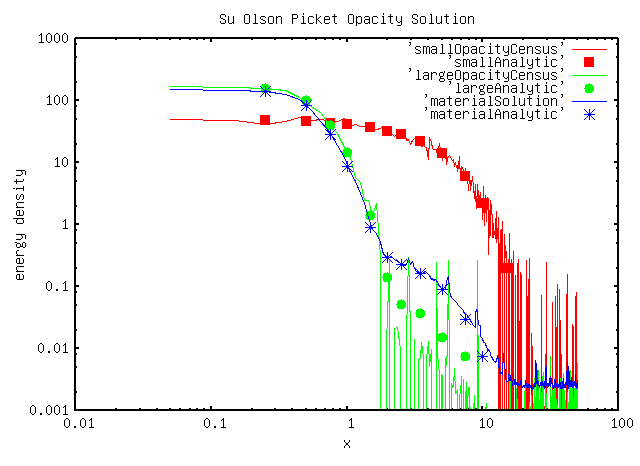
\includegraphics[width=\imgwidth,height=\imgheight]{NG-NDF}}
		\end{picture}
		\caption{\label{fig:NG-NDF} Frequency dependent result without the difference formulation compared to the Su and Olson semi-analytic result[Su 1999]. (Problem 4.1a) }
		\end{minipage} %\hfill
	\end{center}
\end{figure}

\begin{figure}[htbp]
	\unitlength1in
	\begin{center}
		\begin{minipage}[t]{6in}
		\centering
		\begin{picture}(\width,\height)
	                {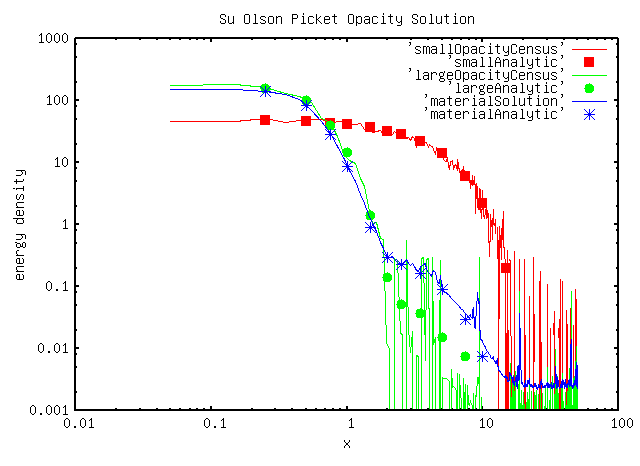
\includegraphics[width=\imgwidth,height=\imgheight]{NG-DF-10}}
		\end{picture}
		\caption{\label{fig:NG-DF-10} Frequency dependent result, using the difference formulation temperature set to 10\% of the material temperature, compared to the Su and Olson semi-analytic result[Su 1999]. (Problem 4.1b) }
		\end{minipage} %\hfill
	\end{center}
\end{figure}

\begin{figure}[htbp]
	\unitlength1in
	\begin{center}
		\begin{minipage}[t]{6in}
		\centering
		\begin{picture}(\width,\height)
	                {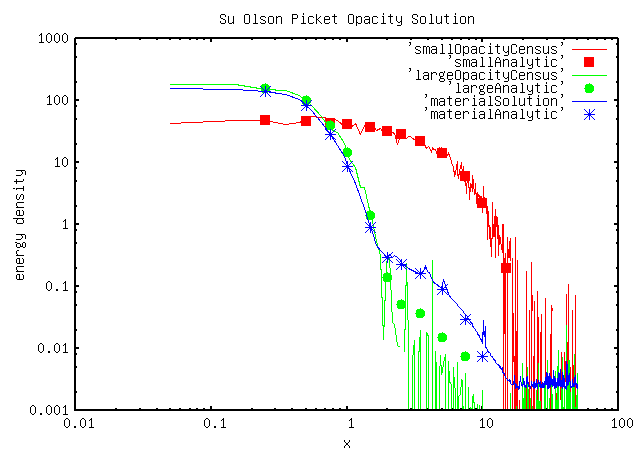
\includegraphics[width=\imgwidth,height=\imgheight]{NG-DF-30}}
		\end{picture}
		\caption{\label{fig:NG-DF-30} Frequency dependent result, using the difference formulation temperature set to 30\% of the material temperature, compared to the Su and Olson semi-analytic result[Su 1999]. (Problem 4.1c) }
		\end{minipage} %\hfill
	\end{center}
\end{figure}

\begin{figure}[htbp]
	\unitlength1in
	\begin{center}
		\begin{minipage}[t]{6in}
		\centering
		\begin{picture}(\width,\height)
	                {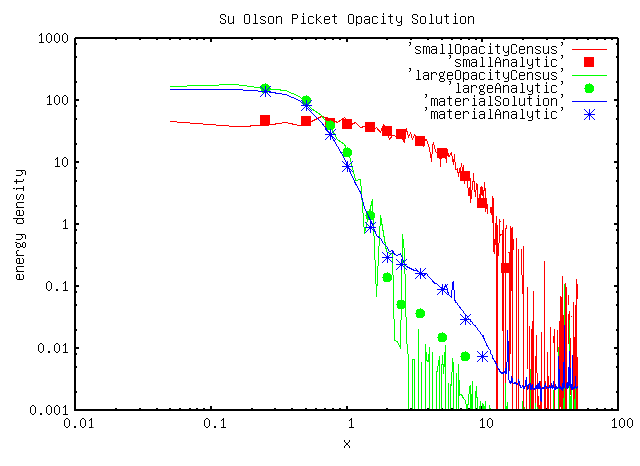
\includegraphics[width=\imgwidth,height=\imgheight]{NG-DF-50}}
		\end{picture}
		\caption{\label{fig:NG-DF-50} Frequency dependent result, using the difference formulation temperature set to 50\% of the material temperature, compared to the Su and Olson semi-analytic result[Su 1999]. (Problem 4.1d) }
		\end{minipage} %\hfill
	\end{center}
\end{figure}

	Figures \ref{fig:NG-NDF}, \ref{fig:NG-DF-10}, \ref{fig:NG-DF-30}, and \ref{fig:NG-DF-50} show the IMD solution with the difference formulation for the various percentages of the difference formulation temperature as compared to the material temperature. The ``smallAnalytic'', ``largeAnalytic'', and ``materialAnalytic'' denote the Su and Olson semi-analytic non-grey benchmark results for the energy density of the small opacity associated photons, large opacity associated photons, and the material, respectively. The material energy density results are displayed for all four realizations of Problem 4.1 in figure \ref{fig:DF-NG-MaterialEnergyDensity}.

\begin{figure}[htbp]
	\unitlength1in
	\begin{center}
		\begin{minipage}[t]{6in}
		\centering
		\begin{picture}(\width,\height)
	                {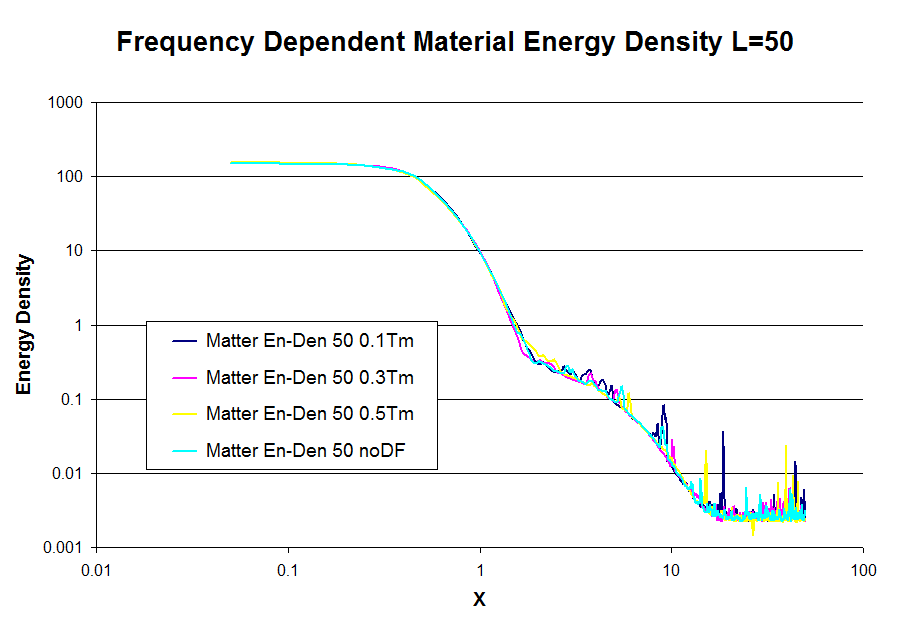
\includegraphics[width=\imgwidth,height=\imgheight]{DF-NG-MaterialEnergyDensity}}
		\end{picture}
		\caption{\label{fig:DF-NG-MaterialEnergyDensity} Non-grey result at various percentages of the material temperature for the difference formulation. (Problem 4.1)}
		\end{minipage} %\hfill
	\end{center}
\end{figure}


	The relative standard deviations associated with the material energy density for the different realizations of Problem 4.1 are shown in Figure \ref{fig:DF-NG-RelSTD50}. The relative standard deviation is simply the standard deviation of the associated cell energy density divided by the value of the energy density in that cell. 

\begin{figure}[htbp]
	\unitlength1in
	\begin{center}
		\begin{minipage}[t]{6in}
		\centering
		\begin{picture}(\width,\height)
	                {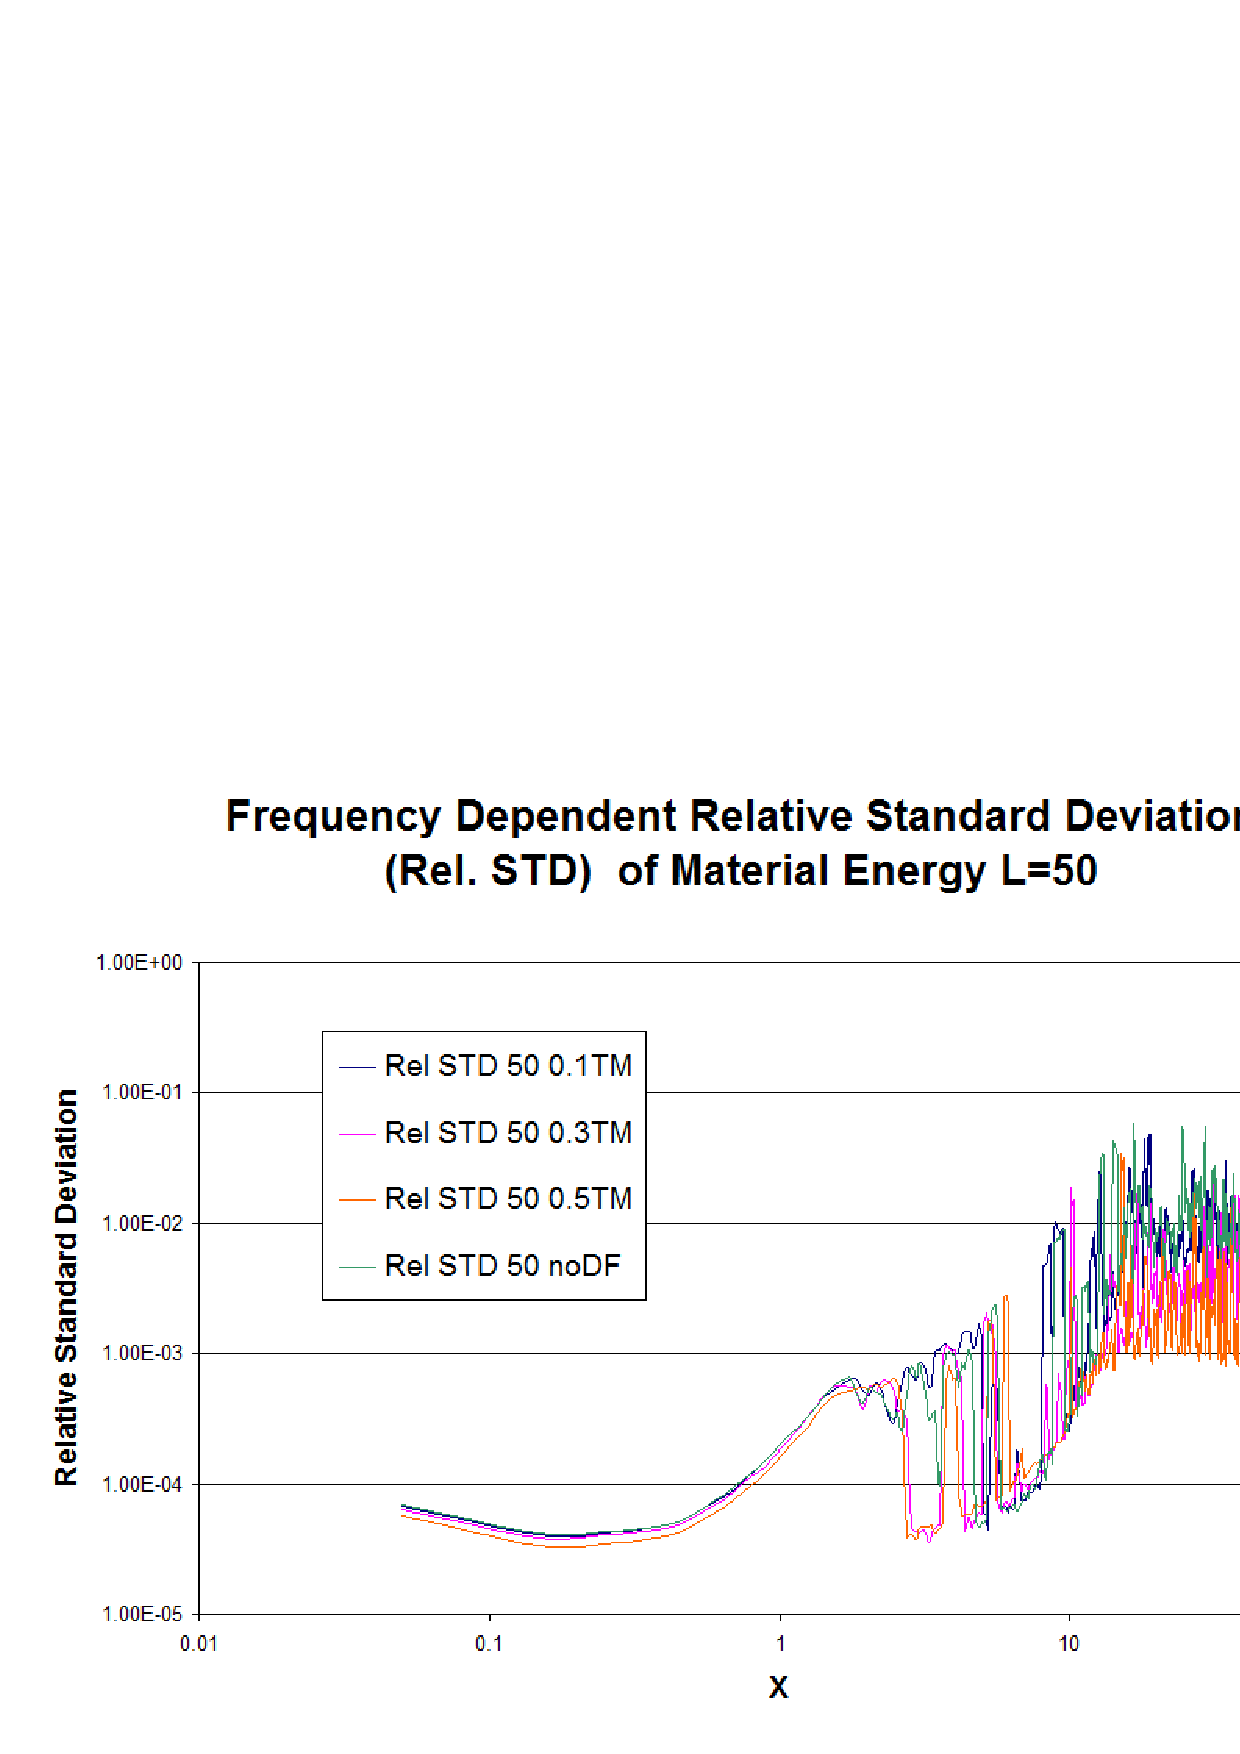
\includegraphics[width=\imgwidth,height=\imgheight]{DF-NG-RelSTD50}}
		\end{picture}
		\caption{\label{fig:DF-NG-RelSTD50} The relative standard deviation of the material energy density for the different realization of Problem 4.1.}
		\end{minipage} %\hfill
	\end{center}
\end{figure}

	In Figure \ref{fig:DF-NG-RelSTD50}, the values associated with ``Rel STD 50 0.1Tm'' denotes the relative standard deviation (Rel STD) of the material energy density with total problem length equal to 50 Mm and the difference formulation temperature equal to 10\% of the material temperature. The other values are defined similarly with the exception of ``Rel STD 50 noDF'' which denotes the solution generated without the difference formulation. 

% 	The figure of merit of each cell's material energy density can be calculated as ${1\over{\sigma^2t}}$ where $\sigma^2$ denotes the variance of the material energy density and $t$ denotes the calculation time. The relative figure of merit is defined for this work as the figure of merit of the material energy density with the difference formulation divided by the figure of merit without the difference formulation for an associated cell. This value can be used to determine the effective decrease in variance as a function of the computational cost. 
% 
% \begin{figure}[htbp]
% 	\unitlength1in
% 	\begin{center}
% 		\begin{minipage}[t]{6in}
% 		\centering
% 		\begin{picture}(\width,\height)
% 	                {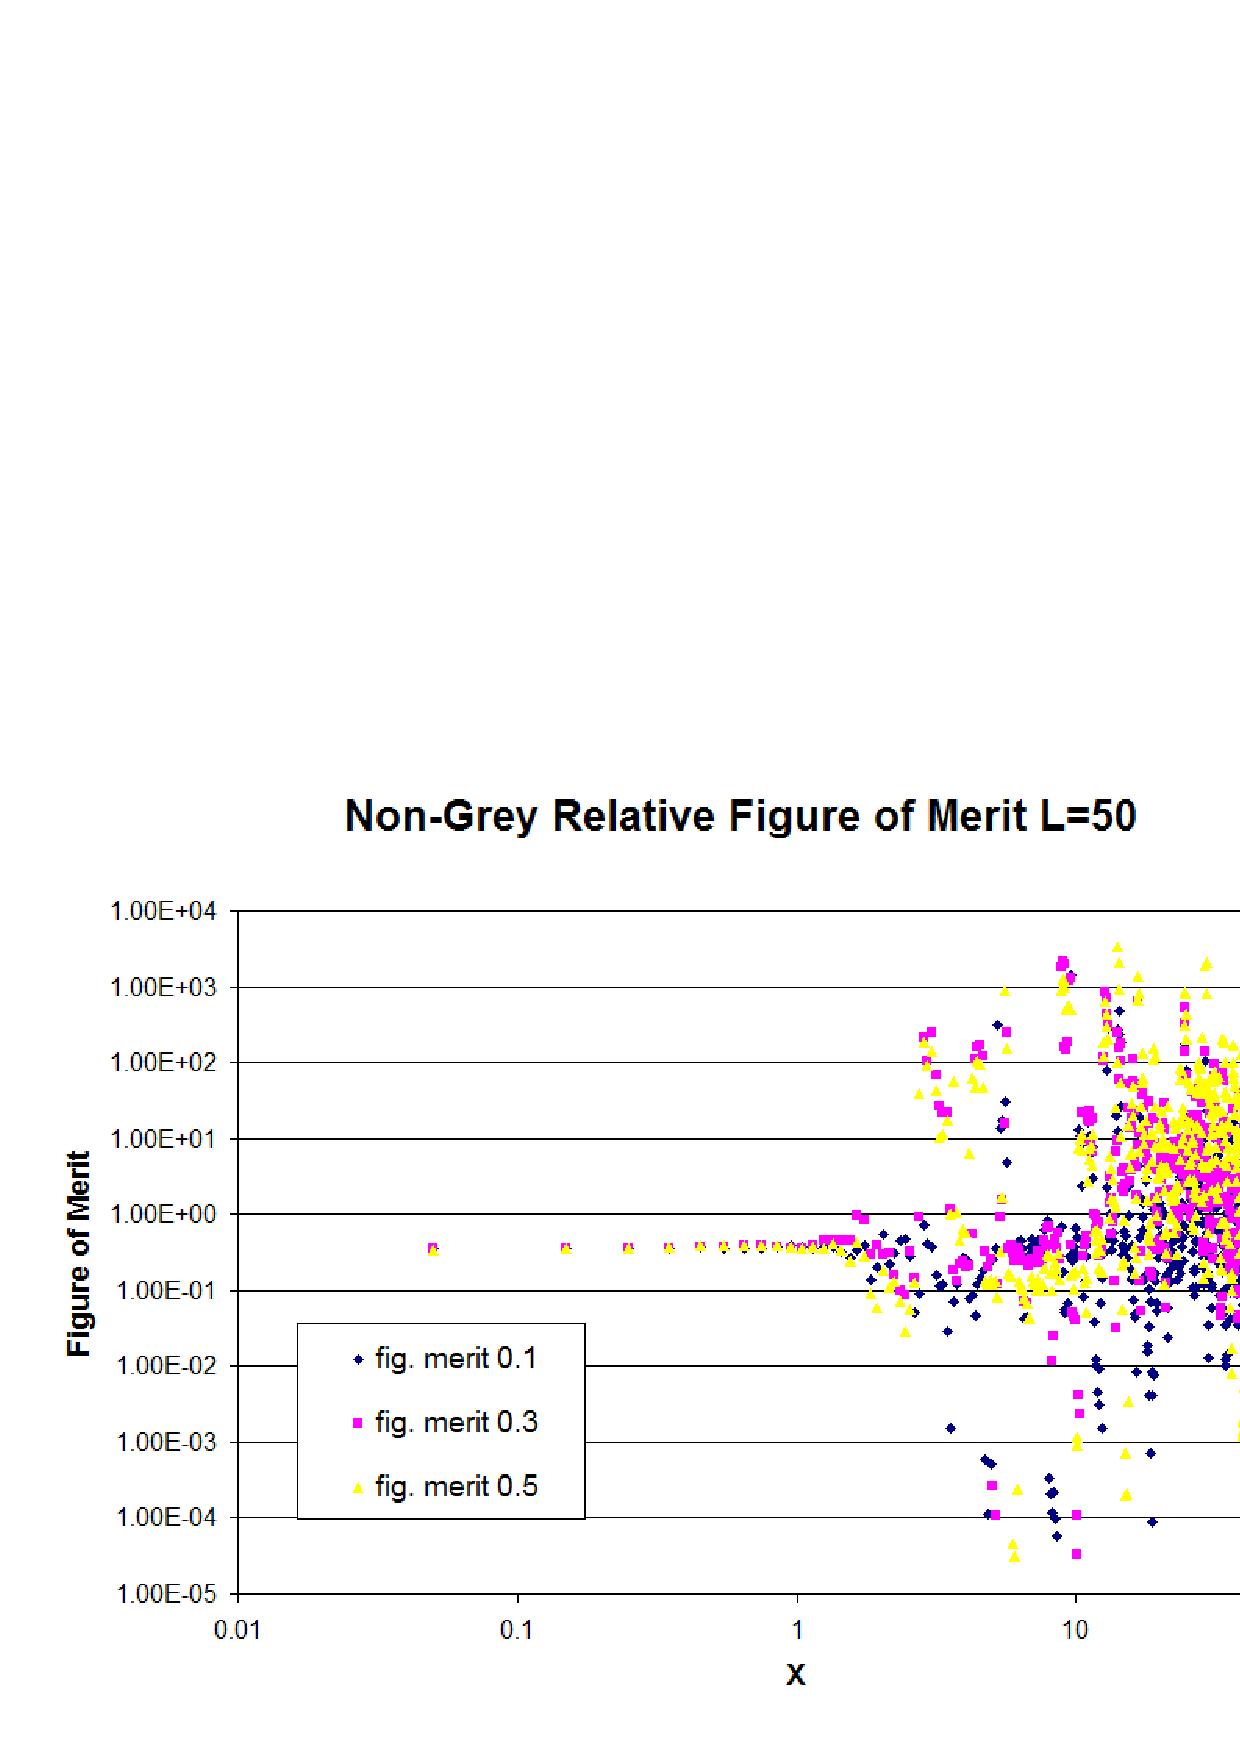
\includegraphics[width=\imgwidth,height=\imgheight]{DF-NG-FigMerit50}}
% 		\end{picture}
% 		\caption{\label{fig:DF-NG-FigMerit50} The relative figure of merit per cell for the difference formulation at various percentages of the material temperature. (Problem 4.1)}
% 		\end{minipage} %\hfill
% 	\end{center}
% \end{figure}
% 		
% 	In Figure \ref{fig:DF-NG-FigMerit50}, it is important to note that this expresses the figure of merit at each cell which is determined from the variance in the associated cell and the total computation time of the problem. It is also important to note that any value of relative figure of merit below one or greater than one demonstrate a relative decrease or increase in the comparative figure of merit respectively.

	For Problem 4.1 the total figure of merit is the sum of the figure of merit for each cell over the whole problem. The associated relative total figure of merit is the total figure of merit associated with a given variance reduction technique divided by the total figure of merit without it. This is expressed for Problem 4.1 in Figure \ref{fig:DF-NG-TotalFigMerit}.

\begin{figure}[htbp]
	\unitlength1in
	\begin{center}
		\begin{minipage}[t]{6in}
		\centering
		\begin{picture}(\width,\height)
	                {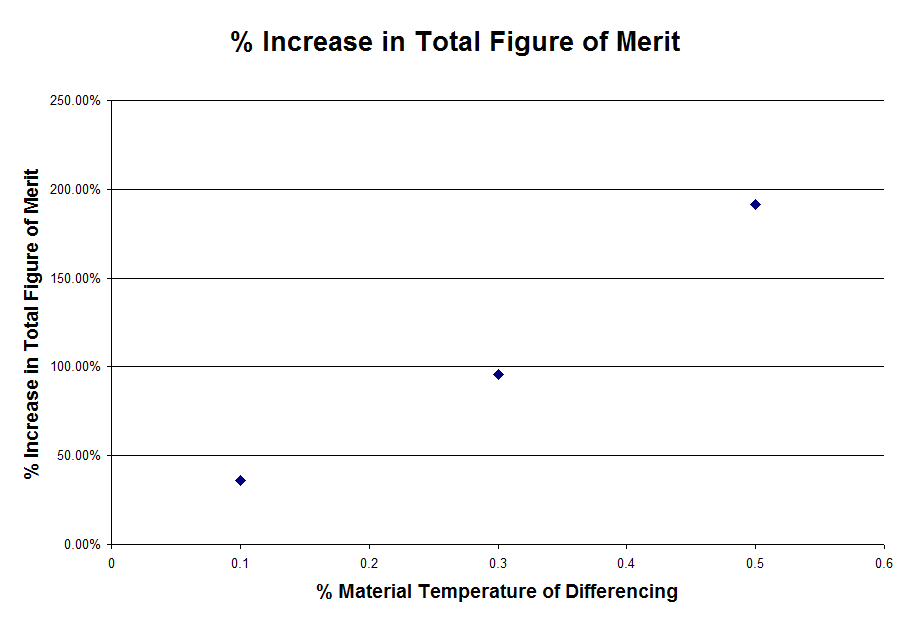
\includegraphics[width=\imgwidth,height=\imgheight]{DF-NG-TotalFigMerit}}
		\end{picture}
		\caption{\label{fig:DF-NG-TotalFigMerit} The relative total figure of merit for the difference formulation at various percentages of the material temperature. (Problem 4.1)}
		\end{minipage} %\hfill
	\end{center}
\end{figure}

% 	Similarly, for Problem 4.1 the average figure of merit is the average figure of merit in each cell over the whole problem. The associated relative average figure of merit is the relative average figure of merit associated with a given variance reduction technique divided by the relative average figure of merit without it. This is expressed for Problem 4.1 in Figure \ref{fig:DF-NG-AveFigMerit}.
% 
% \begin{figure}[htbp]
% 	\unitlength1in
% 	\begin{center}
% 		\begin{minipage}[t]{6in}
% 		\centering
% 		\begin{picture}(\width,\height)
% 	                {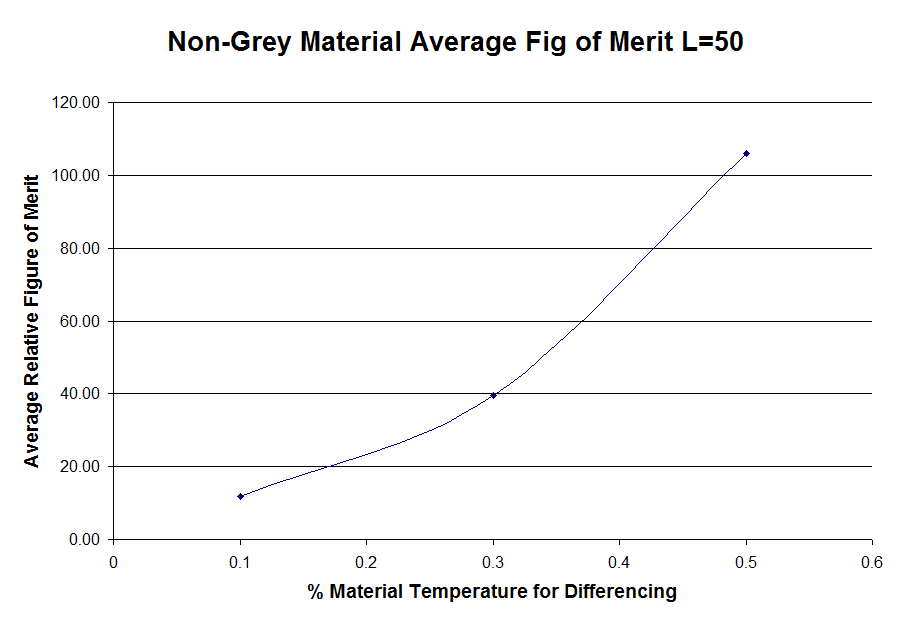
\includegraphics[width=\imgwidth,height=\imgheight]{DF-NG-AveFigMerit}}
% 		\end{picture}
% 		\caption{\label{fig:DF-NG-AveFigMerit} The relative average figure of merit for the difference formulation at various percentages of the material temperature. (Problem 4.1)}
% 		\end{minipage} %\hfill
% 	\end{center}
% \end{figure}

\belowSubSecSkip

%=====================================================================%
% SubSection:                        	                              %
%     Results: Summary %
%=====================================================================%
\subsection{Summary}
\label{sec:Results-Summary}

\noindent
	\indent The results obtained from the grey and frequency dependent calculations were compared to the benchmark semi-analytic results of Su and Olson[Su 1996][Su 1999], with and without the difference formulation. The temporal and spatial resolution dependence was tested for both the grey and frequency dependent IMD methods using five refinements in each independent variable.  The efficiency of the difference formulation at various percentages of the material temperature was tested as a way to reduce the material energy density variance.













%=================================================%
% Section:                        	              %
%    Conclusions %
%=================================================%

\begin{center}
\section{Conclusions}
\label{sec:Conclusions}
\end{center}

%====================================================================%
% SubSection:                        	                             %
%    Conclusions: Introduction %
%====================================================================%
\aboveSubSecSkip

\subsection{Introduction}
\label{sec:Conclusions-Intro}

\noindent
	\indent This chapter will discuss the results presented in Section \ref{sec:Results}. This includes an analsis of the results of the Implicit Monte Carlo Diffusion frequency dependent and grey solutions compared to their associated semi-analytic benchmarks, presented by Su and Olson[Su 1996][Su 1999]. Stability, variance, and accuracy will all be discussed based on the material temperature, because it is generally the most important quantity, particularly in multiphysics applications. The conclusions that can be drawn from the spatial and temporal refinements of the frequency dependent and grey methods will be explained. Similarly, the impact of group refinement on the frequency dependent methods will be be analyzed. The performance of the difference formulation on the benchmark problems will be discussed. The overall variance reduction will be quantified for the frequency dependent IMD method with the difference formulation, including some statements on the stability/instability of the difference formulation and potential problems in its use. 
			
\belowSubSecSkip



%=====================================================================%
% SubSection:                        	                              %
%     Conclusions: IMD with the difference Formulation
%=====================================================================%
\subsection{Implicit Monte Carlo Diffusion without the Difference Formulation}
\label{sec:Conclusions-Non-Grey-IMD}

\noindent
	\indent The development of the grey IMD method was completed for initial testing of the difference formulation. Working with a grey system is simpler then a multigroup system because there is no need to distribute the differenced energy among frequency groups. It can simply be subtracted and added to the total photon energy density. Similarly, there is no need to randomly sample from the frequency distribution of the streaming source obtained from the difference formulation. Though the grey system is a good platform for initial testing it is not a realistic physical model of any radiative transfer applications. The multigroup method was initially tested for on a grey problem by setting the opacity equal to a single value for every frequency.

	The results of Problem 1.1 (Figures \ref{fig:Grey_MW_No_DF_L=50} and \ref{fig:Grey_MG_MW_No_DF_L=50}) show that both IMD codes can accurately reproduce the Su and Olson purely absorbing grey benchmark result[Su 1996]. Both codes, grey and multigroup, produce a significant amount of noise in the low energy regions of the solution. This is related to the relatively small number of particles created in these regions because of the comparative low contribution to the total energy of the system. 

	The results generated from the standard IMD method for Problem 3.1 (Figure \ref{fig:NG-SO}) show that the frequency dependent IMD code can accurately reproduce the results of the semi-analytic picket fence opacity benchmark defined by Su and Olson[Su 1999]. The photon energy density associated with the large opacity (large census $\sigma={200\over{101}}$) is underestimated in the regions between x=2 and the front of the Marshak wave because not enough particles are created in that region to get an accurate distribution of the thermal emission frequencies. There is significantly more noise in the cold region of the problem due to the low overall contribution of energy in those cells.

	The results from Problem 1.2a (Figure \ref{fig:Grey-Spatial-Refinment}) and Problem 3.2a (Figure \ref{fig:NG-Refine-Space}) show the effect of spatial resolution on the accuracy of the material energy density solution. With a relatively coarse spatial mesh, very little shape resolution is lost and the solution remains stable. As the number of particles used to solve the matrix via Monte Carlo approaches infinity, the solution approaches that of the linear system. As a result the Monte Carlo solution will have a spatial accuracy dependent on the discretization scheme used to generate the linear system. 

	The results from Problem 3.2b (Figure \ref{fig:NG-Refine-time1} and Figure \ref{fig:NG-Refine-time2}) show the effect of the time step size on the multigroup IMD method. The results from Problem 1.2b (Figure \ref{fig:Grey-Tempral-Refinment1} and Figure \ref{fig:Grey-Tempral-Refinment2}) indicate a similar effect on the grey IMD method. As the temporal discretization is refined, the penetration distance of the Marshak wave is reduced. This is an effect of the discretization and not the solution method. As the size of the time step increases, the streaming terms become unphysically dominate. This causes the numerically simulated wave front to progress too far into the problem, effectively smearing out the wave front. The changes in the numerical solution from the temporal refinement are also expected to be more drastic (than those seen from the spatial refinement) because the spatial refinement is second order and the temporal refinement is first order.

	It is known that the cost of solving the matrix deterministicly scales linearly with the number of groups used. This is because for every group a new matrix must be solved. This is not the case for the Monte Carlo method. The frequency dependence of the Monte Carlo method is determined via the random sampling from the frequency distribution functions. Figure \ref{fig:NG-MG} shows the computational cost as a function of the number of groups used. The cost per group curve has a slope equal to 1/2 compared to a deterministic method, which would be nearly one. Only a single matrix solution takes place and the frequency distribution is defined by the particle frequency distribution.  
	
	Using a Monte Carlo method for solving the matrix has advantages and disadvantages. The major advantage is there is no need to solve the matrix for each group. However, the solution to the linear system of equations using Monte Carlo takes much longer than the deterministic solution. The goal of developing IMD was to couple it with IMC. Using a Monte Carlo method to solve the diffusion equation has the advantage that it is much easier to couple to the IMC method. Using the criteria defined by Densmore et al, it is possible to transition particles from IMD (or DDMC) to IMC[Den 2007]. For the deterministic solution, the spatial domain must be decomposed and the deterministic solution could only be coupled to the IMC solution at the end of every time step.

	

	

\belowSubSecSkip
%=====================================================================%
% SubSection:                        	                              %
%     Conclusions: IMD without the difference formulation
%=====================================================================%
\subsection{Implicit Monte Carlo Diffusion with the Difference Formulation}
\label{sec:Conclusions-Grey-IMD}

\noindent
	\indent Figure \ref{fig:Grey_MW_DF_L=50} shows the solution to Problem 1.1 using the grey IMD method and the difference formulation. A significant reduction in the variance occurs in the region of the problem where the material is near thermal equilibrium. In fact, on the right side of the Marshak wave no particles are actually transported and the variance incurred from the Monte Carlo method in this region is equal to zero. The energy is simply subtracted off at the beginning of the time step during the initial differencing of the problem. It is then added directly back into the problem at the end of the time step. Like most variance reduction techniques, this reduction in variance comes at a cost. Without the difference formulation, the IMD system defined in this work is unconditionally stable. This is not true for the system with the difference formulation. In standard IMD, there are no negatively weighted particles created. This means that the total energy in any cell can never become less than zero. Equations \ref{leftStreamingSource} and \ref{rightStreamingSource}, which represent the streaming source terms created from the difference formulation, indicate that negative particles will indeed be created. This means that it is possible for more negative weight than positive weight to be deposited into a single cell, causing the overall material temperature to become less than zero. One way to alleviate this is to use absorption and census supression with a very low weight cutoff. These problems demonstrated how unstable the difference formulation can be even for the grey case. The stability appears to be strongly dependent on the number of particles that are used and the spatial gradient of the energy density. When the difference formulation failed, it was at the leading edge of the Marshak wave. It never failed in the large near equilibrium back end of the Marshak wave or the cold portion of the material at thermal equilibrium. In fact even if a vacuum boundary is set on the cold side of the problem, well away from the head of the Marshak wave front, the system was stable. The figure of merit was not determined for the grey case because it would be much higher than that of the frequency dependent difference formulation. The estimation of computational efficiency of the difference formulation was limited to the frequency dependent case.

	The stability of the frequency dependent IMD method with the difference formulation was explored. Problem 4.1 (Figures \ref{fig:NG-DF-10},\ref{fig:NG-DF-30}, and \ref{fig:NG-DF-50}) shows the ability of the frequency dependent IMD method with the difference formulation to solve the Su and Olson picket fence opacity benchmark result[Su 1999]. Figure \ref{fig:DF-NG-MaterialEnergyDensity} shows that three difference formulation solutions with various match the solution without the difference formulation. The variance is reduced as the percentage of the material temperature used for the difference formulation is increased. This will be explored in greater detail later in this section.

	The Problem 4.1 results for the difference formulation with the difference temperature equal to that of the material temperature were not included because of numerical instability. There was also an instability in the cumulative distribution function used to calculate the frequency distribution (equations \ref{CDF_q_d_j-1} and \ref{CDF_q_d_j+1}). This instability exists because the subtraction of two nearly equal numbers when the Plankian distribution for a frequency group is low for both temperatures creating a large roundoff error. Also, if the Planck integral expansion is not accurate, the Planckian for a higher temperature at a given frequency can be lower than that of a lower temperature. This is unphysical because it is known that the Planckian at a higher temperature is larger at every frequency the the Planckian at a lower temperature.

	The relative standard deviation of the material energy density was quantified to determine the effectiveness of the difference formulation at reducing the variance. The relative standard deviation is a measure of the uncertainty of the solution compared to its mean. The relative standard deviation for Problem 4.1 is shown in Figure \ref{fig:DF-NG-RelSTD50}. This figure shows that with the exception of the leading edge of the Marshak wave, the relative standard deviation is consistently lower for the majority of the difference formulation temperatures. This is especially true for the portions of the problem that are near equilibrium (either ahead or behind of the wave front).

% 	To quantify the computational cost of the difference formulation versus the reduction in the variance, the relative figure of merit is calculated as a function of the material energy density location. For any value of the relative figure of merit greater than one there is a performance increase. For any value less than one there is a performance decrease. It can be seen from Figure \ref{fig:DF-NG-FigMerit50} that an increase in the figure of merit is primarily seen in the region of the problem that are near equilibrium and initial very cold. It should be noted that though there was a reduction in the relative standard deviation for the difference formulation, the cost is so expensive that there is an overall performance decrease. This is due impart to the fact that the variance was initially very low in this region of the problem already.

	The total figure of merit is the sum of the material energy density figure of merit overall cells. The increase in the total figure of merit can then be expressed as the total figure of merit of the calculation with the variance reduction technique divided by the total figure of merit without the variance reduction technique. Figure \ref{fig:DF-NG-TotalFigMerit} shows the relative increase in the figure of merit as a function of the percent of the material temperature used for the difference formulation. This figure shows that there is a strong increase in the figure of merit as the percent of the material termperature for the difference formulation is increased. 

% 	Figure \ref{fig:DF-NG-AveFigMerit} demonstrates the increase in the average figure of merit over the problem. The average figure of merit over the problem is simply the average figure of merit over all the cells. The increase in the average figure of merit is simply the average figure of merit with a variance reduction technique divided by the average figure of merit without the variance reduction. It can be seen from this figure that the increase in the average figure of merit is lower than that of the total figure of merit, but is still far greater than one for each case. The increase in the average figure of merit is about half of the increase in the total figure of merit over the problem. This could be linked to the poor increase in the relative figure of merit for the cells on the back side of the Marshak wave front. In looking at figrue \ref{fig:DF-NG-TotalFigMerit} it can be seen that the relative figure of merit for the cells behind the wave front decreases as the difference formulation temperature is increased towards that of the material temperature. This is the opisite of what happens for the regions in front of the wave. There is an overall gain in the relative figure of merit for these cells as the difference formulation temperature is increased towards that of the material temperature. 

\belowSubSecSkip
%=====================================================================%
% SubSection:                        	                              %
%     Conclusions: Overall Conclusions and Future Work%
%=====================================================================%
\subsection{Overall Conclusions and Future Work}
\label{sec:Conclusions-over}

\noindent
	\indent This research shows that frequency dependent IMD can be used to accurately reproduce solutions to the frequency dependent radiative transfer equations where the diffusion approximation is valid. It also shows that frequency dependent IMD is stable if the spatial and temporal discretizations used to generate the linear system are stable. Though this frequency dependent system is solved via IMD, frequency dependent DDMC should also be possible. The primary difference between DDMC and IMD is the treatment of the temporal discretization.
	
	The difference formulation was shown to have some significant advantages and disadvantages when used with IMD. Implimentation of the difference formulation significantly increases the figure of merit in regions of the problem where the system is near equilibrium. However, the difference formulation did become unstable in regions containing sharp gradients. This was associated with the creation of large negatively weighted particles from the streaming source of the difference formulation. These instabilities can be reduced by using a lower temperature for the difference formulation. This reduces the size of the negatively weighted particles being produced by the difference formulation source and it increases the amount of positively weighted particles created by the thermal emission source. 
	
	Several improvements to IMD are left for future work, including the extention of the method on orthogonal meshes beyond one dimensional and two dimensional cylindrical. It will take very little effort to extend this work toward two or three dimensional orthogonal meshes. However, unstructured polyhedral meshes which are commonly used in high density physics, pose difficult problems because of the possible creation of positive off diagonal elements in the coefficient matrix as explained in Section \ref{sec:MonteCarlo-Probabilities}, and in the work of Gentile[Gen. 2001], for the leakage probabilities to be positive the off diagonal elements of the coefficient matrix must be negative. Techniques for matrix manipulation such that all off diagonal elements will be negative will be very important. 

	Improved implementations of the difference formulation should also be explored. This includes automating the use of the difference formulation in different regions of the problem. The goal is to focus the use of the difference formulation where the system is near equilibrium and reduce its use in regions of sharp gradients. More work should also be done to develop an efficient and stable algorithm for the frequency distribution function of the difference formulation streaming source. The majority of the computational work for the difference formulation is associated with the sampling of this source. 











\ResetSingleSpace      % ... back to single-spacing

%==================%
% Section:         %
%    Bibliography  %
%==================%

\addcontentsline{toc}{section}{{}{\refname}}

\begin{thebibliography}{Wac 75}

\vskip0.1in

\bibitem[Ada. 1998]{Ada:1998} Adams, M. L., Nowak, P.F.,
	``Asymptotic analysis of a computational method for time- and frequency- dependent radiative transfer'', 
	\emph{Journal of Computational Physics},
	\textbf{146}, 366-403 (1998).

\bibitem[Bar. 1970]{Bar:1970} Barnett, C., Canfield, E., ``Sampling a random variable distributed according to Planck's law'', \emph{Internal Livermore Document.},

\bibitem[Bro. 1989]{Bro:1989}  Brooks, E. D., ``Symbolic Implicit Monte Carlo'', 
	\emph{Journal of Computational Physics}, 
	\textbf{83(2)}, 433-446 (1989).

\bibitem[Bro. 2005]{Bro:2005} Brooks, E. D., McKinley, M.S., Daffin, F., Szoke, A., ``Symbolic implicit Monte Carlo radiation transport in the difference formulation: a piecewise constant discretization'', \emph{Journal of Computational Physics}, \textbf{205},
	737-754 (2005).

\bibitem[Bro 2006]{Bro:2006} Brooks, E. D., Szoke, A., Peterson, J.D.L., ``Piecewise linear discretization of Symbolic Implicit Monte Carlo radiation transport in the difference formulation'', \emph{Journal of Computational Physics}, , \textbf{220},
	471-497 (2006).
	
\bibitem[Clo 2003]{Clo:2003} Clouet, J. F., Samba, G., ``A hybrid symbolic Monte Carlo method for radiative transfer equations'', \emph{Journal of Computational Physics}, \textbf{188},
	139-156 (2003).

\bibitem[Dud. 1976]{Dud:1976} Duderstadt, J. J. and Hamilton, L. J., \textbf{Nuclear Reactor Analysis}, John Wiley \& Sons, Inc., New York (1976).


\bibitem[Daf 2005]{Daf:2005} Daffin, F., McKinley, M.S., Brooks, E.D., Szoke, A., ``An evaluation of the difference formulation for photon transport in a two level system'', 
	\emph{Journal of Computational Physics},
	\textbf{204},  27-45 (2005).
	
\bibitem[Den 2007]{Den:2007} Densmore, J. D., Urbatsch, T.J., Evans, T.M., Buksas, M.W., ``A hybrid transport-diffusion method for Monte Carlo radiative-transfer simulations'', 
	\emph{Journal of Computational Physics},\textbf{222}, 485-503 (2007).

\bibitem[Fle. 1971]{Fle:1971} Fleck, J. A., Cummings, J.D., ``An implicit Monte Carlo scheme for calculating time and frequency dependent nonlinear radiation transport'',  \emph{Journal of Computational Physics}, \textbf{8}, 313-342 (1971).

\bibitem[Fle. 1984]{Fle:1984} Fleck, J. A., Canfield, E.H., ``A random walk procedure for improving the computational efficiency of the implicit Monte Carlo method for nonlinear radiation transport'', \emph{Journal of Computational Physics}, \textbf{54(3)}, 508-523 (1984).
	

\bibitem[Gen 2001]{Gen:2001} Gentile, N. A., ``Implicit Monte Carlo Diffusion - An acceleration method for Monte Carlo time-dependent radiative transfer simulations'', 
	\emph{Journal of Computational Physics},
	\textbf{172}, 543-571 (2001).	

\bibitem[Gen. 2006]{Gen:2006} Gentile, N. A., ``The difference formulation of radiation transport in implicit Monte Carlo, invited'', 
	\emph{Transactions of the American Nuclear Society },
	\textbf{95}, 871-872 (2006).

\bibitem[Ham. 1964]{Ham:1964} Hamerssley, J. M. and Handscomb, D. C., \textbf{Monte Carlo methods}, John Wiley \& Sons, Inc., New York (1964).
	
\bibitem[Inc. 2002]{Inc:2002} Incropera, F. P. and DeWitt, D. P., \textbf{Fundamentals of heat and mass transfer-5th ed.}, John Wiley \& Sons, Inc., New York (2002). 


\bibitem[Lar 1983]{Lar:1983} Larsen, E. W., Pomraning, G.C., Badham, V.C., ``Asymptotic analysls of radiative transfer problems. Journal of Quantitative Spectroscopy and Radiative Transfer'',  \emph{Journal of Quantitative Spectroscopy and Radiative Transfer}, \textbf{29(4)}, 
	285-310 (1983).

\bibitem[Lew. 1993]{Lew:1993} Lewis, E. E. and Miller, Jr. D. P., \textbf{Computational Methods of Neutron Transport}, American Nuclear Society, Inc., Illinois (1993). 


\bibitem[McK 2002]{McK:2002} McKinley, M. S., Brooks, E.D., Szoke, A., ``Comparison of Implicit and Symbolic Implicit Monte Carlo Line Transport with Frequency Weight Vector Extension'', \emph{Internal Livermore Document}, (2002). 	
	
\bibitem[N'Ka 1991]{N'Ka:1991} N'Kaoua, T., ``Solution of the nonlinear radiative transfer equations by a fully implicit matrix Monte Carlo method coupled with the Rosseland diffusion equation via domain decomposition'',
	\emph{SIAM Journal on Scientific and Statistical Computing}, \textbf{2(3)}, 505-520 (1991).
	
\bibitem[Su 1996]{Su:1996} Su, B., Olson, G.L., ``Benchmark results for the non-equilibrium Marshak diffusion problem'', \emph{Journal of Quantitative Spectroscopy and Radiative Transfer}, \textbf{56(3)}, 337-351(1996).

\bibitem[Su 1997]{Su:1997} Su, B., Olson, G.L., ``An analytical benchmark for non-equilibrium radiative transfer in an isotropically scattering medium'', \emph{Annals of Nuclear Energy}, \textbf{24(13)}, 1035-1055 (1997).

\bibitem[Su 1999]{Su:1999} Su, B., Olson, G.L., ``Non-grey benchmark results for two temperature non-equilibrium radiative transfer'', \emph{Journal of Quantitative Spectroscopy and Radiative Transfer}, \textbf{62}, 279-302(1999).
	
\bibitem[Szi 1992]{Szi:1992} Szilard, R. H., Pomraning, G.C., ``Numerical transport and diffusion methods in radiative transfer'',
	\emph{Nuclear Science and Engineering}, \textbf{112}, 256-269 (1992).

\bibitem[Szo 2005]{Szo:2005} Szoke, A., Brooks, E.D., ``The transport equation in opitically thick media'', 
	\emph{Journal of Quantitative Spectroscopy and Radiative Transfer}, \textbf{91}, 95-110 (2005).

\end{thebibliography}




%=================================================================%

%=====================%
% End of the document %
%=====================%

\end{document}
